\documentclass[10pt]{memoir}
\setstocksize{220mm}{155mm} 	        
\settrimmedsize{220mm}{155mm}{*}	
\settypeblocksize{170mm}{116mm}{*}	
\setlrmargins{18mm}{*}{*}
\setulmargins{*}{*}{1.2}
%\setlength{\headheight}{5pt}%
\checkandfixthelayout[lines]
\linespread{1.16}
\flushbottom

%%% Hyphenation settings
\usepackage[htt]{hyphenat}
\hyphenation{he-lio-trope opos-sum}
\tracingparagraphs=1
%Hyphenation in Devanāgarī of the edition still missing? Probably this needs to be modified in babel-iast package? 

%%% babel
\usepackage[english]{babel}
\usepackage{babel-iast/babel-iast}

\babelfont[iast]{rm}[Renderer=Harfbuzz, Scale=1.3]{AdishilaSan}%AdishilaSan}
\babelfont[english]{rm}{Adobe Text Pro}

%%% more functionality
\PassOptionsToPackage{hyphens}{url}
\usepackage{hyperref}
\usepackage{pdflscape}
\usepackage{cleveref}
\usepackage{url}
\usepackage{cleveref}
\usepackage{microtype}
\usepackage{lineno}

%\usepackage{bigfoot}
%%% more functions
\usepackage[dvipsnames]{xcolor}
%\usepackage[para,perpage]{footmisc}

%%%für den Counter von Kapiteln und Sätzen! 
\newcommand{\uproman}[1]{\uppercase\expandafter{\romannumeral#1}}
\newcommand{\lowroman}[1]{\romannumeral#1\relax}

\makeindex
\newfontfamily\sanskritfont[Script=Devanagari,Mapping=RomDev,Scale=1.1]{Sanskrit2003}
\usepackage{pifont,fourier-orns,lettrine,psvectorian,paralist,enumitem,pdfpages,wrapfig,tabulary,lettrine,longtable}
\setlist[enumerate]{itemsep=0mm}
\usepackage[autostyle]{csquotes}
\usepackage[defaultlines=2,all]{nowidow}
\usepackage{ellipsis,adforn,booktabs,longtable,url,tikz}
\lineskiplimit=-3pt          

\makechapterstyle{IeT}{%
  \chapterstyle{default}
  \renewcommand*{\printchapternonum}{\centering}
  \renewcommand*{\clearforchapter}{\cleartorecto} 
  \aliaspagestyle{chapter}{empty}}
\chapterstyle{IeT}
\setsecnumdepth{none}  \openright  \nouppercaseheads
\settocdepth{subsubsection}

%%%% test better pagebreaks
%\def\fussy{%
%  \emergencystretch\z@
%  \tolerance 200%
%  \hfuzz .1\p@
%  \vfuzz\hfuzz}

%\interfootnotelinepenalty=10000\relax

%\usepackage[maxfloats=256]{morefloats}

%\maxdeadcycles=500

%raggedbottomsectiontrue
%%\checkandfixthelayout


%%%%%%%  biblatex
%\newcommand{\noun}[1]{\textsc{#1}}    %  philosophy-verbose
\usepackage[backend=biber, sorting=nyt, style=verbose]{biblatex} %%%%ORIGINAL TiE
\renewcommand*{\mkbibnamefamily}[1]{\textsc{#1}}


\DeclareFieldFormat{url}{%
  \mkbibacro{URL}\addcolon\space
  \href{#1}{\nolinkurl{\thefield{urlraw}}}}

\DeclareFieldFormat{citeurl}{%
  \href{#1}{\nolinkurl{\thefield{urlraw}}}} 


\DeclareFieldFormat{postnote}{#1}
\renewcommand{\postnotedelim}{, }
\addbibresource{bindu.bib}

%%% ekdosis
\usepackage[teiexport=tidy,parnotes=true]{ekdosis}% =tidy cleans up HTML and XML documents by fixing markup errors and upgrading legacy code to modern standards. parnotes=footnotes below or above critical apparatus

\SetLineation{lineation=page, modulo} %lineation=page sets thenumbering to start afresh at the top of each page. =modulo makes every fifth line numbered. {lineation=page} makes every line numbered! 

\renewcommand{\linenumberfont}{\selectlanguage{english}\footnotesize} %sets language of lines to English

\SetTEIxmlExport{autopar=false} %autopar=falseinstructs ekdosis to ignore blank lines in the.tex sourcefile as markers for paragraph boundaries. As a result, each paragraph of the edition must be found within an environment associated with the xml <p> element

\SetHooks{
  lemmastyle=\bfseries,
  %refnumstyle=\selectlanguage{english}\bfseries,
  refnumstyle=\selectlanguage{english}\color{blue}\bfseries,
  appheight=0.8\textheight,
}

\newif\ifinapparatus
\DeclareApparatus{source}[
%bhook=\inapparatustrue,
lang=english,
notelang=english,
% bhook=\selectlanguage{english},
bhook=\selectlanguage{english}\textbf{Sources:},%
%maxentries=4, 
%ehook=.]
%sep={] },
%nosep,
]

\newif\ifinapparatus
\DeclareApparatus{testium}[
%bhook=\inapparatustrue,
lang=english,
notelang=english,
% bhook=\selectlanguage{english},
bhook=\selectlanguage{english}\textbf{Testimonia:},
%maxentries=4, 
%ehook=.]
%nosep, 
]

% Declare \ifinapparatus and set \inapparatustrue at the beginning of
% the apparatus criticus block. Also set the language.  
\newif\ifinapparatus
  \DeclareApparatus{default}[
  %bhook=\inapparatustrue, 
  lang=english,
  %maxentries=33,
  %bhook=\selectlanguage{english},
  sep = {] },
  delim=\hskip 0.75em,
  rule=\rule{0.7in}{0.4pt},
]

\newif\ifinapparatus
\DeclareApparatus{philcomm}[
%bhook=\inapparatustrue,
lang=english,
notelang=english,
bhook=\selectlanguage{english}\textbf{Philological Commentary:},
%bhook=\selectlanguage{english},
sep={: },
]

\ekdsetup{
showpagebreaks,
spbmk = \textcolor{blue}{spb},
hpbmk = \textcolor{red}{hpb}
}

%\usepackage{fnpos}
%\makeFNmid
%\makeFNbottom
\usepackage[bottom]{footmisc}
%%%%%%%%%%%%%%%%%%%%%%%%%%%
\makeatletter
\def\blfootnote{\gdef\@thefnmark{}\@footnotetext}
\makeatother
%%%%%%%%%%%%%%%%%%%%%%%%%


% Macros and Definitions for the Print of Sigla
\def\acpc#1#2#3{{#1}\rlap{\textrm{\textsuperscript{#3}}}\textsubscript{\textrm{#2}}\space}
\def\sigl#1#2{{{#1}}\textsubscript{\textrm{#2}}}
\def\None{{\sigl{N}{1}}} \def\Noneac{\acpc{N}{1}{ac}\,} \def\Nonepc{\acpc{N}{1}{pc}\,}
\def\Ntwo{{\sigl{N}{2}}} \def\Noneac{\acpc{N}{2}{ac}\,} \def\Nonepc{\acpc{N}{2}{pc}\,}
\def\Done{{\sigl{D}{1}}} \def\Doneac{\acpc{D}{1}{ac}\,} \def\Donepc{\acpc{D}{1}{pc}\,}
\def\Dtwo{{\sigl{D}{2}}} \def\Dtwoac{\acpc{D}{2}{ac}\,} \def\Dtwopc{\acpc{D}{2}{pc}\,}
\def\Uone{{\sigl{U}{1}}} \def\Uoneac{\acpc{U}{1}{ac}\,} \def\Uonepc{\acpc{U}{1}{pc}\,}                 
\def\Utwo{{\sigl{U}{2}}} \def\Utwoac{\acpc{U}{2}{ac}\,} \def\Utwopc{\acpc{U}{2}{pc}\,}

%%%%%%%%%%%%%% Tattvabinduyoga - List of Witnesses   %%%%%%%%%%%%%%%%%%%
\DeclareWitness{ceteri}{\selectlanguage{english}cett.}{ceteri}[]   
\DeclareWitness{E}{\selectlanguage{english}E}{Printed Edition}[]    
\DeclareWitness{P}{\selectlanguage{english}P}{Pune BORI 664}[]  
\DeclareWitness{B}{\selectlanguage{english}B}{Bodleian 485}[]       
\DeclareWitness{N1}{\selectlanguage{english}N\textsubscript{1}}{NGMPP 38/31}[]
\DeclareWitness{N2}{\selectlanguage{english}N\textsubscript{2}}{NGMPP B 38/35}[]
\DeclareWitness{L}{\selectlanguage{english}L}{LALCHAND 5876}[]  
\DeclareWitness{D}{\selectlanguage{english}D}{IGNCA 30019}[] 
%\DeclareWitness{D2}{\selectlanguage{english}D\textsubscript{2}}{IGNCA 30020}[]  
\DeclareWitness{U1}{\selectlanguage{english}U\textsubscript{1}}{SORI 1574}[] 
\DeclareWitness{U2}{\selectlanguage{english}U\textsubscript{2}}{SORI 6082}[]
%%%%%%%%%%%%%% Tattvabinduyoga - Groups of Witnesses   %%%%%%%%%%%%%%%%%%%
\DeclareWitness{X}{\selectlanguage{english}\alpha}{Alpha Group: D,N1,N2,U1}[]
\DeclareWitness{Y}{\selectlanguage{english}\beta}{Beta Group: B,E,L,P,U2}[]
%%%%%%%%%%%%% Testimonia
\DeclareWitness{Ysv}{\selectlanguage{english}Ysv}{Yogasvarodaya}[] %%%add infos!  

%%%%%%%%%%%%%%%%%%%%%%%%%%%%%%%%%%%%%%%%%%%
% Macro for Editing Abbrevs.
\def\om{\textrm{\footnotesize \textit{om.}\ }} %prints om. for omitted in apparatus
\def\korr{\textrm{\footnotesize \textit{em.}\ }} %prints em. for emended in apparatus
\def\conj{\textrm{\footnotesize \textit{conj.}\ }} %prints conj. for conjectured in apparatus

% \supplied{text} EDITORIAL ADDITION -> Within \lem oder \rdg
% \surplus{text} EDITORIAL DELETION -> Within \lem oder \rdg
% \sic{text} CRUX
% \gap{text} LACUNAE -> [reason=??, unit=??, quantity=??, extent=??]


%%%%%%%%%%%%%%%%%%%%%%%%%%%%%%%%%%%%%%%%%%% All macros of this list can be used in 
% Macro for Editing Abbrevs.
\def\eyeskip{\textrm{{ab.\,oc. }}}
\def\aberratio{\textrm{{ab.\,oc. }}}
\def\ad{\textrm{{ad}}}
\def\add{\textrm{{add.\ }}}
\def\ann{\textrm{{ann.\ }}}
\def\ante{\textrm{{ante }}} 
\def\post{\textrm{{post }}}
%\def\ceteri{cett.\,}                   
\def\codd{\textrm{{codd.\ }}}

\def\coni{\textrm{{coni.\ }}}
\def\contin{\textrm{{contin.\ }}}
\def\corr{\textrm{{corr.\ }}}
\def\del{\textrm{{del.\ }}}
\def\dub{\textrm{{ dub.\ }}}

\def\expl{\textrm{{explic.\ }}} 
\def\explica t{\textrm{{explic.\ }}}
\def\fol{\textrm{{fol.\ }}}
\def\foll{\textrm{{foll.\ }}}
\def\gloss{\textrm{{glossa ad }}}
\def\ins{\textrm{{ins.\ }}}      
\def\inseruit{\textrm{{ins.\ }}} 
\def\im{{\kern-.7pt\lower-1ex\hbox{\textrm{\tiny{\emph{i.m.}}}\kern0pt}}} %\textrm{\scriptsize{i.m.\ }}}      
\def\inmargine{{\kern-.7pt\lower-.7ex\hbox{\textrm{\tiny{\emph{i.m.}}}\kern0pt}}}%\textrm{\scriptsize{i.m.\ }}}      
\def\intextu{{\kern-.7pt\lower-.95ex\hbox{\textrm{\tiny{\emph{i.t.}}}\kern0pt}}}%\textrm{\scriptsize{i.t.\ }}}           
\def\indist{\textrm{{indis.\ }}}  
\def\indis{\textrm{{indis.\ }}}
\def\iteravit{\textrm{{iter.\ }}} 
\def\iter{\textrm{{iter.\ }}}
\def\lectio{\textrm{{lect.\ }}}   
\def\lec{\textrm{{lect.\ }}}
\def\leginequit{\textrm{{l.n. }}} 
\def\legn{\textrm{{l.n. }}}
\def\illeg{\textrm{{l.n. }}}

\def\primman{\textrm{{pr.m.}}}
\def\prob{\textrm{{prob.}}}
\def\rep{\textrm{{repetitio }}}
\def\secundamanu{\textrm{\scriptsize{s.m.}}}            \def\secm{{\kern-.6pt\lower-.91ex\hbox{\textrm{\tiny{\emph{s.m.}}}\kern0pt}}}%   \textrm{\scriptsize{s.m.}}}
\def\sequentia{\textrm{{seq.\,inv.\ }}}  
\def\seqinv{\textrm{{seq.\,inv.\ }}}
\def\order{\textrm{{seq.\,inv.\ }}}
\def\supralineam{{\kern-.7pt\lower-.91ex\hbox{\textrm{\tiny{\emph{s.l.}}}\kern0pt}}} %\textrm{\scriptsize{s.l.}}}
\def\interlineam{{\kern-.7pt\lower-.91ex\hbox{\textrm{\tiny{\emph{s.l.}}}\kern0pt}}}   %\textrm{\scriptsize{s.l.}}}
\def\vl{\textrm{v.l.}}   \def\varlec{\textrm{v.l.}} \def\varialectio{\textrm{v.l.}}
\def\vide{\textrm{{cf.\ }}}
\def\cf{\textrm{{cf.\ }}} 
\def\videtur{\textrm{{vid.\,ut}}}
\def\crux{\textup{[\ldots]} }
\def\cruxx{\textup{[\ldots]}}
\def\unm{\textit{unm.}}
%%%%%%%%%%%%%%%%%%%%%%%%%%%%%%%%%%%%

% List of Scholars
\DeclareScholar{ego}{ego}[
forename=Nils Jacob,
surname=Liersch]

% Persons:14\DeclareScholar{ego}{ego}[15forename=Robert,16surname=Alessi]17% Useful shorthands:18\DeclareShorthand{codd}{codd.}{V,I,R,H}19\DeclareShorthand{edd}{edd.}{Lit,Erm,Sm}20\DeclareShorthand{egoscr}{\emph{scripsi}}{ego}

%Useful shorthands:
%\DeclareShorthand{codd}{codd.}{V,I,R,H}
%\DeclareShorthand{edd}{edd.}{Lit,Erm,Sm}
\DeclareShorthand{egoscr}{em.}{ego}
\DeclareShorthand{egoscrconj}{conj.}{ego}
\DeclareShorthand{egomute}{\unskip}{ego}

\usepackage{xparse}

\NewDocumentEnvironment{tlg}{O{}O{}}{\setlength{\leftskip}{0pt}\vspace{-1ex}\begin{quotation}}{\hfill #1\ \vspace{-1ex}\end{quotation}\vspace{-1ex}} %verse environment
%\NewDocumentEnvironment{tlg}{O{}O{}}{\begin{verse}}{॥#1\hskip-4pt ॥\\ \end{verse}}
\NewDocumentCommand{\tl}{m}{{\selectlanguage{iast} #1}}

\NewDocumentCommand{\extra}{m}{{\textcolor{gray}{#1}}} %command for additions to U2
\NewDocumentCommand{\crazy}{m}{{\textcolor{red}{#1}}} %totally corrupted passage
\NewDocumentCommand{\coro}{m}{{\textcolor{violet}{#1}}} %colour for sentence counter! 

\NewDocumentEnvironment{prose}{O{}}{\begin{otherlanguage}{iast}}{\end{otherlanguage}}
% \NewDocumentEnvironment{padd}{O{}}{\begin{otherlanguage}{iast}}{\end{otherlanguage}}
\NewDocumentEnvironment{tlate}{O{}}
%\NewDocumentEnvironment{tadd}{O{}}

%Define two commands: \skp ("sanskrit plus"), to be ignored by TeX in
%the edition text, but processed in the TEI output. Conversely, \skm
%("sanskrit minus") is to be processed in the edition text, but
%ignored if found in the apparatus criticus and in the TEI output:

\NewDocumentCommand{\skp}{m}{}
\TeXtoTEIPat{\skp {#1}}{#1}

%\NewDocumentCommand{\skpp}{m}{}
%\TeXtoTEIPat{\skpp {#1}}{#1}

\NewDocumentCommand{\skm}{m}{\unless\ifinapparatus#1-\fi}
\TeXtoTEIPat{\skm {#1}}{}

% \NewDocumentCommand{\dd}{}{/\hskip-4pt/}
\NewDocumentCommand{\dd}{}{\mbox{/\hskip-4pt/}}
\TeXtoTEIPat{\dd {}}{//}


%%% modify environments and commands
%%% TEI mapping
\TeXtoTEIPat{\begin {tlg}}{<lg>} %lg=(Group of verse (s)) contains one or more verses or lines of verse that together form a formal unit (e.g. stanza, chorus).
\TeXtoTEIPat{\end {tlg}}{</lg>}

\TeXtoTEIPat{\begin {prose}}{<p>}
\TeXtoTEIPat{\end {prose}}{</p>}

\TeXtoTEIPat{\begin {tlate}}{<p>}
\TeXtoTEIPat{\end {tlate}}{</p>}

\TeXtoTEIPat{\\}{}
\TeXtoTEIPat{\linebreak}{<br/>}
\TeXtoTEIPat{\noindent}{}
%\TeXtoTEI{tl}{l}
\TeXtoTEI{emph}{hi}
\TeXtoTEI{bigskip}{}
\TeXtoTEI{None}{N1}
\TeXtoTEI{Ntwo}{N2}
\TeXtoTEI{Done}{D1}
\TeXtoTEI{Dtwo}{D2}
\TeXtoTEI{Uone}{U1}
\TeXtoTEI{Utwo}{U2}
%\TeXtoTEIPat{/}{ |}
%\TeXtoTEI{//}{ ||}
\TeXtoTEIPat{\korr}{em. }
\TeXtoTEIPat{\conj}{conj.}
\TeXtoTEIPat{\om}{om.}
\TeXtoTEIPat{english}{}
\TeXtoTEIPat{\hskip}{}
\TeXtoTEIPat{\hskip-4pt}{}
\TeXtoTEIPat{\hskip-2pt}{}
\TeXtoTEIPat{-}{ }
\TeXtoTEIPat{4pt}{}
\TeXtoTEIPat{2pt}{}
\TeXtoTEIPat{\textcolor {#1}{#2}}{<hi rend="#1">#2</hi>} 

% Nullify \selectlanguage in TEI as it has been used in
% \DeclareWitness but should be ignored in TEI.
\TeXtoTEI{selectlanguage}{}



\FormatDiv{1}{\begin{center}\Large}{\end{center}}
\FormatDiv{2}{\begin{center}\small}{\end{center}}
\FormatDiv{3}{\bfseries}{.}
\title{Yogatattvabindu of Rāmacandra\\ A Critical Edition and Annotated Translation}
\date{\today}

\parindent=15pt
\begin{document}

%Zitiermöglichkeiten:
%\footcite[See][p.\,1]{goldstein01:_tibet_englis_diction_moder_tibet}
%\footnote{\cite{goldstein01:_tibet_englis_diction_moder_tibet}.}

\frontmatter
\thispagestyle{empty}
\begin{center}
  {\Large \emph{The Yogatattvabindu}}\\[3mm]
\end{center}



\newpage

\

\thispagestyle{empty}



\normalsize


\newpage


\begin{center}
\thispagestyle{empty}

\

\vskip 2mm

\begin{otherlanguage}{iast}
\LARGE \sanskritfont{Yogatattvabindu}
\end{otherlanguage}

\vskip .4cm

\Huge Yogatattvabindu \\[7mm]
\Large Critical Edition\\
and annotated Translation\\
together with a Comparative Analysis of the \\Complex Early Modern Yoga Yaxonomies 


\large

\vspace{3cm}

By

Nils Jacob Liersch
\small
\vfill

\vfill

Indica et Tibetica Verlag \\ % $\cdot$ 
Marburg 2024

\vskip 6mm

\end{center}

\newpage
\newpage \ \thispagestyle{empty}
\small  \

\noindent

\
\vfill


\small
\noindent \textbf{Bibliographische Information Der Deutschen Bibliothek}

\noindent
Die Deutsche Bibliothek verzeichnet diese Publikation in der Deutschen Nationalbibliographie;
detaillierte bibliographische Informationen sind im Internet über http://dnb.ddb.de abrufbar.

\noindent
\textbf{Bibliographic information published by Die Deutschen Bibliothek}

\noindent
Die Deutsche Bibliothek lists this publication in the Deutsche Nationalbibliographie; detailed
bibliographic data is available in the Internet at http://dnb.ddb.de.  


\vskip 1cm

\noindent
\copyright\ Indica et Tibetica Verlag, Marburg 2024

\medskip

\noindent
Alle Rechte vorbehalten / All rights reserved

\medskip

\noindent
Ohne ausdrückliche Genehmigung des Verlages ist es nicht gestattet, das Werk oder einzelne Teile
daraus nachzudrucken, zu vervielfältigen oder auf Datenträger zu speichern.

\smallskip

\noindent
Apart from any fair dealing for the purpose of private study, research, criticism or review, no
part of this book may be reproduced or translated in any form, by print, photo form, microfilm, or
any other means without written permission. Enquiries should be made to the publishers.

\bigskip

\noindent
Satz: \ \ Nils Jacob Liersch \\
Herstellung: \ \ BoD – Books on Demand GmbH, Norderstedt  \\

\bigskip

\noindent
%\ISBN     

\normalsize

\newpage

%\maketitle
\clearpage
\tableofcontents
\addtocounter{page}{-1}
\thispagestyle{empty}
\clearpage


\mainmatter

\chapter{Conventions in the Critical Apparatus}
\section{Sigla in the Critical Apparatus}

\begin{itemize}
\item E : Printed Edition
\item P : Pune BORI 664
\item L : Lalchand Research Library LRL5876
\item B : Bodleian Oxford D 4587
‚\item \None : NGMPP B 38-31
\item \Ntwo : NGMPP B 38-35 / A 1327-14
\item \Done : IGNCA 30019
\item \Uone : SORI 1574
\item \Utwo: SORI 6082
\end{itemize}

\chapter{Critical Edition \& Annotated Translation}
\cleardoublepage
\begin{alignment}[
  texts=edition[class="edition"];
  translation[class="translation"],
  ]
  \begin{edition}
    \ekddiv{
      head={[\uproman{33}. \textbf{piṇḍamadhye lokatrayam}]},
      type=section,
      depth=2, 
      n=XXXIII
    }
    \xmlhead[h33]{[XXXI. piṇḍamadhye lokatrayam]}
\label{lokatraya}
    \begin{prose}[p33_01]
        \noindent
%----------------------------
%idānīṃ                    śarīramadhye lokatrayaṃ kathyate/  mūlādhāre bhūrlokaḥ/  liṃgāgre  bhuvarlokaḥ/  liṃgamadhye  svarlokaḥ//    \E
%idānīṃ                    piṃḍamadhye  lokatrayaṃ kathyate   mūlādhāre bhūrlokaḥ   liṃgāgre  bhuvarlokaḥ   liṃgamūle    svarlokaḥ      \P
%idānīṃ                    piḍopiri     lokatrayaṃ kathyate// mūlādhāre bhūrlokaḥ   liṃgāgre  bhuvarloka----liṃgamadhye  svarlokaḥ//    \B
%idānīṃ                    piṃḍopari    lokatrayaṃ kathyate// mūlādhāre bhūrlokaḥ// liṃgāgre  bhuvarloka----liṃgamadhye  svarlokaḥ//   \L
%idānīṃ                    piṃḍamadhye  lokatrayaṃ kathyate/  mūlādhāre bhūrlokaḥ/  liṃgamūle                            svarlokaḥ     \N1
%idānīṃ                    piṃḍamadhye  lokatrayaṃ kathyate// mūlādhāre bhūrlokaḥ// liṃgāgre  bhuvarlokaḥ// liṃgamadhye  svarlokaḥ//   \D
%idānīṃ                    piṃḍamadhye  lokatrayaṃ kathyate/  mūlādhāre bhūrlokaḥ   liṃgamūle                            svargalokaḥ// \N2
%idānīṃ upari tataṃ  lokaṃ piṃḍamadhye  lokatrayaṃ kathyate   mūlādhāre bhūrlokaḥ   liṃgāgre  bhuvarlokaḥ   liṃgamūle    svaravarlokaḥ \U1
%idānīṃ                    piṃḍamadhye  lokatrayaṃ kathyate// mūlādhāre bhūrlokaḥ// liṃgāgre  bhuvarlokaḥ// liṃgamūle    svarlokaḥ//   \U2
%-----------------------------
%Now the threefold world within the body is taught. The earth is situated at the root support (\textit{mūladhāra}). The airspace is at the tip of the penis. Heaven is inside of the penis. 
%----------------------------
\note[type=source, labelb=266, labele=_266e, nosep]{cf. YSv (PT p. 842): idānīṃ piṇḍamadhye tu saptalokaṃ śṛṇu priye | mūlādhāre tu bhūrloko liṅgāgre tu bhuvas tataḥ | svarloko liṅgamūle tu merumūle mahas tathā |}
\note[type=testium, labelb=267, labele=_266e, nosep]{cf. SSP 3.3 (Ed. p. 49): bhūrloko guhyasthāne bhuvarloko liṅgasthāne svarlokaṃ nābhisthāne evaṃ lokatraye indro devatā piṇḍamadhye sarvendriyaniyāmakaḥ sa evendraḥ |}
\app{\lem[wit={ceteri}]{idānīṃ}
  \rdg[wit={U1}]{idānīṃ upati tataṃ lokaṃ}}
\app{\lem[wit={ceteri}]{piṇḍamadhye}
  \rdg[wit={L}]{piṃḍopari}
  \rdg[wit={B}]{piḍopiri}
  \rdg[wit={E}]{śarīramadhye}}
lokatrayaṃ kathyate/ mūlādhāre bhūrlokaḥ/
\app{\lem[wit={ceteri}]{liṅgāgre}
  \rdg[wit={N1,N2}]{liṃgamūle}}
\app{\lem[wit={D,E,P,U1,U2}]{bhuvarlokaḥ}
  \rdg[wit={B,L}]{bhuvarloka°}
  \rdg[wit={N1,N2}]{\om}}/
\app{\lem[wit={P,U1,U2}]{liṃgamūle}
  \rdg[wit={B,D,L}]{liṅgamadhye}
  \rdg[wit={N1,N2}]{\om}}
\app{\lem[wit={ceteri}]{svarlokaḥ}
  \rdg[wit={N2}]{svargalokaḥ}
  \rdg[wit={U1}]{svaravarlokaḥ}}\dd{}\linelabel{_266e}
\end{prose}
\ekddiv{
  head={[\uproman{34}. \textbf{uparitanaṃ lokacatuṣkam}]},
  type=section,
  depth=2, 
  n=XXXIV
}
\xmlhead[h34]{[XXXIV. uparitanaṃ lokacatuṣkam]}
\label{quadrupletofworlds}
    \begin{prose}[p34_01]
      \noindent
%----------------------------
%idānīm   uparitanaṃ lokacatuṣka      kathyate/  pṛṣṭhadaṃḍāṃkure  maharlokaḥ/   daṇḍacchidramadhye janalokaḥ/  taddaṇḍanāḍīmadhye   tapolokaḥ/  daṇḍamalamadhye   satyalokaḥ/ \E
%idānīm   uparitanu--lokacatuṣkaṃ     kathyate   pṛṣṭhadaṃḍākūre   maharlokaḥ    daṃḍaschidramadhye janalokaḥ   taddaṃḍanālimadhye   tapolokaḥ   daṃḍakamalamadhye satyalokaḥ \P
%idānīm   uparitanu--lokaḥ catuṣṭayaṃ kathyate// daṃḍaṣṭaṭheṃskure maharlokā/    daṇḍachidramadhye  janaloka    taddaṃḍanālikāmadhye ..polokaḥ   daṇḍakamalamadhye satyalokaḥ// \B
%idānīm   uparitana--lokaḥ catuṣṭayaṃ kathyate// daṃḍaṣṭaṭheṃkure  maharlokaḥ/   daṇḍachidramadhye  janaloka    taddaṃḍatālikāmadhye tapolokaḥ   daṇḍakamalamadhye satyalokaḥ// \L
%idānīṃ   uparijanaṃ lokacatuṣkaṃ     kathyate/  pṛṣṭhadaṃḍāṃkure  maharllokaḥ/  daṇḍacchidramadhye janalokaḥ/  taddaṇḍanālī \om                                               \N1!!!!!!!!!!!!!!!important omission stemmapoint S.11 verso
%idānīṃ// uparitanaṃ lokacatuṣkaṃ     kathyate// pṛṣṭhadaṃḍāṃkure  maharlokaḥ    daṇḍachidramadhye  janalokaḥ// taddaṇḍanālamadhye   tapolokaḥ// daṇḍakamalamadhye satyalokaḥ// \D
%idānīṃ   uparijanaṃ lokacatuṣkaṃ     kathyate// pṛṣṭhadaṃḍākūle   maharllokaḥ/  uchidramadhye      janalokaḥ/  taddaṇḍanālī                                              \om  \N2 !!!!!!!!!!!!!!!!!!important omission stemmapoint
%idānīṃ   uparitanaṃ lokaṃ catuṣkaṃ   kathyate   pṛṣṭhadaṃḍāṃkure  maharlokaḥ    daṃḍasthitamadhye  janalokaḥ   taddaṇḍanāḍīmadhye   tapolokaḥ   daṇḍamalamadhye   satyalokaḥ \U1
%idānīṃ   uparitana--lokacatuṣkaṃ     kathyate// pṛṣṭhadaṃḍāṃkure  maharlokaḥ//  daṃḍachidramadhye  janalokaḥ// daṇḍanālimadhye      tapolokaḥ// daṇḍakamalamadhye satyalokaḥ// \U2
%-----------------------------
%Now, the tetrad of the upper worlds will be taught. The great world (\textit{maharloka}) is at the shoot of the staff of the back. The world of men is in the centre of the cavity of the spine. In the centre of the tube of that spine is the world of \crazy{heat?} (\textit{tapoloka}). In the center of the lotus of the spine is the world of truth. 
%-----------------------------
\note[type=source, labelb=268, labele=_268e, nosep]{cf. YSv (PT p. 842): merucchidre janoloko merunāḍyāṃ tapas tathā | kamale marttyalokas tu iti lokaḥ pṛthak pṛthak | bhūrbhuvaḥsvarmahaś ceti janaś caiva tapas tathā | saptamaḥ satyalokas tu saptaloka iti smṛtaḥ | saptalokais tu pātālair bhuvanāni caturdaśa |}
\note[type=testium, labelb=269, labele=_268e, nosep]{cf. SSP 3.4 (Ed. p. 49): daṇḍāṅkure maharlokaḥ daṇḍakuhare janolokaḥ | daṇḍanāle tapolokaḥ | mūlakamale satyalokaḥ |}
idānīṃ
\app{\lem[wit={D,E,U1}]{uparitanaṃ}
  \rdg[wit={L,U2}]{uparitana°}
  \rdg[wit={N1,N2}]{uparijanaṃ}
  \rdg[wit={P,B}]{uparitanu°}}
\app{\lem[wit={D,P,N1,N2,U2}]{lokacatuṣkaṃ}
  \rdg[wit={E}]{lokacatuṣka}
  \rdg[wit={B,L}]{lokaḥ catuṣṭayaṃ}
  \rdg[wit={U1}]{lokaṃ catuṣkaṃ}}
kathyate/
\app{\lem[wit={ceteri}]{pṛṣṭhadaṇḍāṅkure}
  \rdg[wit={N2}]{pṛṣṭhadaṃḍākūle}
  \rdg[wit={P}]{pṛṣṭhadaṃḍākūre}
  \rdg[wit={B}]{daṃḍaṣṭaṭheṃskure}
  \rdg[wit={L}]{daṃḍaṣṭaṭheṃkure}}
\app{\lem[wit={ceteri}]{maharlokaḥ}
   \rdg[wit={B}]{maharlokā}}/
 \app{\lem[wit={ceteri}, alt={daṇḍachidra°}]{daṇḍachidra}
   \rdg[wit={P}]{daṃḍaschidra°}
   \rdg[wit={U1}]{daṃḍasthita°}
   \rdg[wit={U2}]{uchidra°}}madhye
 \app{\lem[wit={ceteri}]{janalokaḥ}
   \rdg[wit={B,L}]{janaloka}}/\\
\app{\lem[wit={ceteri},alt={taddaṇḍa°}]{taddaṇḍa}
  \rdg[wit={U2}]{daṇḍa°}
}\app{\lem[wit={E,U1},alt={°nāḍīmadhye}]{nāḍīmadhye}
  \rdg[wit={P,U2}]{°nālimadhye}
  \rdg[wit={B}]{°nālikāmadhye}
  \rdg[wit={L}]{°tālikāmadhye}
  \rdg[wit={B}]{°nālamadhye}
  \rdg[wit={N1,N2}]{°nālī}}
\note[type=philcomm, labelb=270, lem={taddaṇḍanāḍīmadhye \ldots}]{After section \uproman{34} up until section \uproman{48}, approximately 25\% of the entire text disappears in the two most important witnesses of the α-group. The two Nepalese manuscripts N\textsubscript{1} and N\textsubscript{2} exhibit a substantial lacuna, which further suggests their close affiliation. They must both be derived from the same exemplar. The omissions of the readings of N\textsubscript{1} and N\textsubscript{2} will not be documented in the apparatus until after their respective gaps to prevent an unnecessarily inflated critical apparatus with entries for every omitted word. The reader will be informed in this apparatus layer once their evidence resumes.}
\label{gapn1n2start}
\app{\lem[wit={ceteri}]{tapolokaḥ}
  \rdg[wit={B}]{polokaḥ}}/ 
\app{\lem[wit={ceteri}]{daṇḍakamalamadhye}
   \rdg[wit={E,U1}]{daṇḍamalamadhye}}
 satyalokaḥ\dd{}\linelabel{_268e}
    \end{prose}
  \end{edition}
  \begin{translation}
        \ekddiv{
          head={[\uproman{33}. \textbf{Triad of worlds}]},
          type=section,
          depth=2, 
          n=XXXIII.1
        }
        \xmlhead[h33]{[XXXIII. Triad of worlds]}
\begin{tlate}[p33_01]
  \noindent
Now, the threefold world within the body is taught.\footnote{The earliest conception of the equation of the cosmos with the body is found in \citetitle{rigveda} 10,90. This concept becomes linked with yogic practice in subsequent Hindu traditions. According to the \textit{Bhagavadgītā} and the \textit{Kūrma Purāṇa}, the deities Viṣṇu and Śiva are described as engaging in the practice of Yoga. During this practice, they assimilate all external aspects by either encompassing the entire universe within their cosmic bodies or by engulfing everything, see \citeauthor[2011:88]{white2011}. For a detailed exposition of the Purāṇic concept of the universe in Patañajli's Yoga, see the commentaries on \citetitle{aranya} 3.25, i.e., \citeauthor[1983: 297-304]{aranya} or \citeauthor[2009:353-356]{bryant2009}. The idea of situating the universe into the yogic body is carried on into the traditions of Haṭha- and Rājayoga and becomes a substantial constituent of their worldview, cf. \citetitle{asiddhi} 15-19.} The earth realm (\textit{bhūrloka}) is situated at the root support (\textit{mūladhāra}). The athmosphere (\textit{bhuvarloka}) is at the tip of the penis. Heaven (\textit{svarloka}) exsits at the base of the penis.
\end{tlate}
\ekddiv{
  head={[\uproman{34}. \textbf{Tetrad of the upper worlds}]},
  type=section,
  depth=2, 
  n=XXXIV.1
}
\xmlhead[h34]{[XXXIV. Tetrad of the upper worlds]}
\begin{tlate}[p34_01]
Now, the tetrad of the upper worlds is taught. The great world (\textit{maharloka}) is at the shoot of the staff of the back. The world of men (\textit{janaloka}) is in the centre of the cavity of the spine. In the centre of the tube of that spine is the world of ascetic heat (\textit{tapoloka}). In the centre of the lotus of the spine is the world of truth (\textit{satyaloka}).\footnote{For a lengthy presentation of Hindu cosmography and their inhabitants, see \citetitle{bhagavata} 5.16-26 or \citetitle{vayupurana} 5.39.}
\flushpage 
\end{tlate}
  \end{translation}
\end{alignment}
\pagebreak % after pp. 85-86
%%%%%%%%%%%%%%%%%%%%%%%%%%%%%%%%%%%%%%%%%%
%%%%%%%%%%%%%%%%%%%%%%%%%%%%%%%%%%%%%%%%%% 
%%%%%%%%PAGEBREAK%%%%%%%PAGEBREAK%%%%%%%%%
%%%%%%%%%%%%%%%%%%%%%%%%%%%%%%%%%%%%%%%%%% 
%%%%%%%%%%%%%%%%PAGEBREAK%%%%%%%%%%%%%%%%%
%%%%%%%%%%%%%%%%%%%%%%%%%%%%%%%%%%%%%%%%%% 
%%%%%%%%PAGEBREAK%%%%%%%PAGEBREAK%%%%%%%%%
%%%%%%%%%%%%%%%%%%%%%%%%%%%%%%%%%%%%%%%%%% 
%%%%%%%%%%%%%%%%%%%%%%%%%%%%%%%%%%%%%%%%%% 
%%%%%%%%%%%%%%%%%%%%%%%%%%%%%%%%%%%%%%%%%% 
%%%%%%%%%%%%%%%%%%%%%%%%%%%%%%%%%%%%%%%%%% 
%%%%%%%%PAGEBREAK%%%%%%%PAGEBREAK%%%%%%%%%
%%%%%%%%%%%%%%%%%%%%%%%%%%%%%%%%%%%%%%%%%% 
%%%%%%%%%%%%%%%%PAGEBREAK%%%%%%%%%%%%%%%%%
%%%%%%%%%%%%%%%%%%%%%%%%%%%%%%%%%%%%%%%%%% 
%%%%%%%%PAGEBREAK%%%%%%%PAGEBREAK%%%%%%%%%
%%%%%%%%%%%%%%%%%%%%%%%%%%%%%%%%%%%%%%%%%% 
%%%%%%%%%%%%%%%%%%%%%%%%%%%%%%%%%%%%%%%%%% 
%%%%%%%%%%%%%%%%%%%%%%%%%%%%%%%%%%%%%%%%%% 
%%%%%%%%%%%%%%%%%%%%%%%%%%%%%%%%%%%%%%%%%% 
%%%%%%%%PAGEBREAK%%%%%%%PAGEBREAK%%%%%%%%%
%%%%%%%%%%%%%%%%%%%%%%%%%%%%%%%%%%%%%%%%%% 
%%%%%%%%%%%%%%%%PAGEBREAK%%%%%%%%%%%%%%%%%
%%%%%%%%%%%%%%%%%%%%%%%%%%%%%%%%%%%%%%%%%% 
%%%%%%%%PAGEBREAK%%%%%%%PAGEBREAK%%%%%%%%%
%%%%%%%%%%%%%%%%%%%%%%%%%%%%%%%%%%%%%%%%%% 
%%%%%%%%%%%%%%%%%%%%%%%%%%%%%%%%%%%%%%%%%%UZU3 
\begin{alignment}[
  texts=edition[class="edition"];
  translation[class="translation"],
  ]
  \begin{edition}
    \ekddiv{
      head={[\uproman{35}. \textbf{catvāro lokasvāminaḥ}]},
      type=section,
      depth=2, 
      n=XXXV
    }
    \xmlhead[h35]{[XXXV. catvāro lokasvāminaḥ]}
    \begin{prose}[p35_01]
      \noindent
%----------------------------
%atha brahmāṇḍamadhye caturdaśa-lokāni sthānāni tānyapi piṃḍe varttante// \E
%atha brahmāṇḍamadhye caturdaśa-lokāsthānāni    tānyapi piḍe  varttate  \P
%atha brahmāṇḍamadhye caturdaśa-lokasthānānī    tānyapi piṃḍo vartate... \B
%atha brahmāṇḍamadhye caturdaśa-lokasthānānī    tānyapi piṃḍe vartate... \L
%\om                                                                 \N1
%atha brahmāṇḍamadhye catvāro   lokasvāminaḥ//  te pi piṃḍamadhye varttate \D %%%p. 14 recto
%\om                                                                 \N2
%atha brahmāṇḍamadhye catvāro   lokāḥ svāminaḥ  te pi piṃḍamadhye vartate \U1
%atha brahmāṇḍamadhye caturddaśalokāḥ stānāni// tānyapi piṃḍe vartate// \U2 %%418.jpg
%-----------------------------
%Now, the locations of the fourteen worlds within the universe exist in the body.
%Now the four lords of the worlds of the external universe also exist in the internal universe.       
%-----------------------------
atha brahmāṇḍamadhye
\app{\lem[wit={D,U1}]{catvāro}
  \rdg[wit={ceteri}]{caturdaśa°}}
\app{\lem[wit={D}]{lokasvāminaḥ}
  \rdg[wit={U1}]{lokāḥ svāminaḥ}
  \rdg[wit={B,L,P}]{°lokāsthānāni}
  \rdg[wit={U2}]{°lokāḥ stānāni}
  \rdg[wit={E}]{°lokāni sthānāni}}/
\app{\lem[wit={E,U1}, alt={te 'pi}]{te\skp{-}'pi}
  \rdg[wit={ceteri}]{tānyapi}}
\app{\lem[wit={E,U1}]{piṇḍamadhye}
  \rdg[wit={B,E,L,U2}]{piṇḍe}
  \rdg[wit={P}]{piḍe}}
\app{\lem[wit={E}]{vartante}
  \rdg[wit={ceteri}]{vartate}}/
%----------------------------
%śarīramadhye  dvau kukṣī  dve sakthinī   vakṣaḥsthalaṃ   kaṃṭhamūlaṃ    kaṃṭhamadhyaṃ laṃbikāmūlaṃ   tāludvāraṃ tālumadhyaṃ     lalāṭamadhye   śṛṃgāṭikā    kapolamadhye   kamalinīmadhye   brahmaraṃdhra             kamalinya---strikūṭasthānam/ \E
%śarīramadhye  dvau kukṣī  dve sakṭhi??nī vakṣaḥ schalaṃ  kaṃṭhamūlaṃ    kaṃṭhamadhyaḥ laṃbikāmūlaṃ   tāludvāraṃ tālumadhye      lalāṭamadhyaṃ  śṛṃgāṭikā    kapolamadhye   kamalinīmadhye   brahmaraṃdhraṃ   ūrddhvaṃ kamalinyā   strikūṭasthānam \P %%%7658.jpg
%śarīramadhye//dvau kukṣau dve sakṭhinī   vakṣaḥsthalaṃ   kaṃṭhamūlaṃ    kamardhye     laṃbikāmūlaṃ   tāludvāraṃ tālumadhyaṃ     lalāṭamadhyaṃ//śṛṃgāṭikā//  kapolamadhye// kamalinīmadhyaṃ  brahmaraṃdhraṃ            kamalīnyāṃ  strikūṭasthānam// \B
%śarīramadhye  dvau kukṣau dve sakthinī   vakṣasthalaṃ    kaṃṭhamūle     kaṃṭhamadhyaṃ laṃbikāmūlaṃ   tāludvāraṃ tālamadhyaṃ     lalāṭamadhyaṃ  śṛṃgāṭikā    karālamadhye   kamalinīmadhyaṃ  brahmaraṃdhraṃ   ūrdhvaṃ  kamalīnyā   trikūṭasthānam... \L
%\om                                                                 \N1
%śarīramadhye  dvau kukṣīnau vartatte//   vakṣasthale//   kaṃṭhasya mūle kaṃṭhamadhye  laṃbikāyāmūle/ tāludvāre tālumadhye       lalāṭe//       śṛṃgāṭikāyāṃ kapolamadhye// kamalinīmadhye// brahmaraṃdhre//  ūrdhva---kamalinyaḥ//trikūṭasthāne// saptapātāle//\D
%\om                                                                 \N2
%śarīramadhye  dvau kukṣīṇau    varttate  vakṣasthale     kaṃṭhasya mūle kaṃṭhamadhye   laṃbikāyāmūle tāludvāre tālumadhye       lalāṭe         śṛṃgāṭikāyāṃ kapolamadhye   kamalinīmadhye   brahmaraṃdhre    urdhva---kamalinyaḥ  trikūṭasthāne... \U1  %%%%287.jpg
%śarīramadhye  dvau kukṣī  dve sakthinī// vakṣassthalaṃ/  kaṃṭhamūle//   kaṃṭhamadhyaḥ//laṃbikāmūlaṃ//tāludvāraṃ// tālumadhyaṃ// lalāṭamadhyaṃ// śrṛṃgāṭikā  kapolamadhye// kamalinīmadhye// brahmaraṃdhraṃ// urdhva---kamalinyās  trikūṭasthānam// \U2
%-----------------------------
%Within the body in the two cavities (1), within the two thighs (2), at the location of the chest (3), at the root of throat (4), in the center of the throat (5) at the root of the uvula (6) at the entrance of the palate (7) at the forehead (8) at the crossroad of the center of the cheecks (9), at the center of the lotuspond (10?), at the aperture of Brahman (11), at the place of the three peaks above the lotusses (14), in the seven hells (21) \ldots
%----------------------------
\note[type=source, labelb=272, labele=_272e, nosep]{cf. YSv (PT p. 842): atha brahmāṇḍamadhyasthāś catvāro lokapālakāḥ | piṇḍamadhye tu tān jñātvā sarvasiddhīśvaro bhavet | indro brahmā viṣṇur īśaś catvāraś cātmadevatāḥ | mūlādhāre catuṣpatre gajārūḍho mahān iti | sṛṣṭikarttā ca tatraiva svādhiṣṭhāne mahān hariḥ | maṇipūre śūlapāṇiraṣṭasiddhīśvaro mahān | tāludvāre tālumadhye lalāṭe vakṣakaṇṭhake | śṛṅgāṭikā kapāle ca lambikā brahmarandhrake | navacakram ūrddhvacakrañ ca trikūṭety ekaviṃśatiḥ | brahmāṇḍāni vasantīti jñātavyāni prayatnataḥ |}
\note[type=source, labelb=273, labele=_272e, nosep]{cf. SSP 3.4-5 (Ed. pp. 50-53): evaṃ lokacatuṣṭaye brahmā devatā | piṇḍamadhye anekamānābhimānasvarūpī tiṣṭhati | viṣṇulokaḥ kukṣau tiṣṭhati | tatra viṣṇur devatā | piṇḍamadhye 'nekavyāpārakārako bhavati | hṛdaye rudralokaḥ | tatra rudro devatā | piṇḍamadhya ugrasvarūpī tiṣṭhati | vakṣaḥsthala īśvaralokaḥ tatreśvaro devatā | piṇḍamadhye tṛptisvarūpī tiṣṭhati | kaṇṭhamūle sadāśivalokaḥ tatra sadāśivo devatā piṇḍamadhye saumyarūpī tiṣṭhati | kaṇṭhamadhye nīlakaṇṭhalokaḥ tatra nīlakaṇṭho devatā | piṇḍamadhye 'bhayasvarūpī tiṣṭhati | tāludvāre śivalokaḥ | tatra śivo devatā | piṇḍamadhye 'nupamasvarūpī tiṣṭhati | lambikāmūle bhairavalokaḥ | tatra bhairavo devatā | piṇḍamadhye sarvottamasvarūpī tiṣṭhati | tatrābhyantare mahāsiddhalokaḥ | tatra mahāsiddhadevatā | piṇḍamadhye prabodhasvarūpī tiṣṭhati | lalāṭamadhye 'nādilokaḥ | lalāṭamadhye ’nādilokaḥ | tatrānādir devatā | piṇḍamadhya ānandaparāhantāsvarūpī tiṣṭhati | śṛṅgaṭe kulalokaḥ | tatra kuleśvaro devatā | piṇḍamadhya ānandasvarūpī tiṣṭhati | śaṅkhamadhye nalinīsthāne 'kuleśalokaḥ | tatra akuleśvaro devatā | piṇḍamadhye nirabhimānāvasthā tiṣṭhati | brahmarandhre parabrahmalokaḥ | tatra parabrahmadevatā | piṇḍamadhye paripūrṇadaśā tiṣṭhati | ūrdhvakamale parāparalokaḥ | tatra parameśvaro devatā | piṇḍamadhye parāparabhāvas tiṣṭhati | trikūṭasthāne śaktilokaḥ | tatra parāśaktir devatā | piṇḍamadhye 'stivāvasthā sarvāsāṃ sarvakartṛtvāvasthā tiṣṭhati | evaṃ piṇḍamadhye saptapātālasahitaikaviṃśatibrahmāṇḍasthānavicāraḥ |}
\begin{otherlanguage}{english}\textbf{\Large{\sic*{}}}\end{otherlanguage}
śarīramadhye
\app{\lem[wit={B,L}]{dvau kukṣau}
  \rdg[wit={E,P,U2}]{dvau kukṣī}
  \rdg[wit={D}]{dvau kukṣīnau}
  \rdg[wit={U1}]{dvau kukṣīṇau}}\dd{}
\app{\lem[wit={E,L,U2}]{dve sakthinī}
  \rdg[wit={P,B}]{dve sakṭhinī}
  \rdg[wit={D,U1}]{vartate}}\dd{}
\app{\lem[type=emendation, resp=egoscr]{vakṣaḥsthale}
  \rdg[wit={D,U1}]{vakṣasthale}
  \rdg[wit={E,B}]{vakṣaḥ sthalaṃ}
  \rdg[wit={P}]{vakṣaḥschalaṃ}
  \rdg[wit={U2}]{vakṣassthalaṃ}}
\app{\lem[wit={L,U2}]{kaṇṭhamūle}
  \rdg[wit={E,P,B}]{kaṃṭhamūlaṃ}
  \rdg[wit={D,U1}]{kaṃṭhasya mūle}}\dd{}
\app{\lem[wit={D,U1}]{kaṇṭhamadhye}
  \rdg[wit={B}]{kamardhye}
  \rdg[wit={E,L}]{kaṃṭhamadhyaṃ}
  \rdg[wit={P,U2}]{kaṃṭhamadhyaḥ}}\dd{}
\app{\lem[type=emendation, resp=egoscr]{lambikāmūle}
  \rdg[wit={D,U1}]{laṃbikāyā mūle} %laṃbikāyām mūle = locatives
  \rdg[wit={ceteri}]{laṃbikāmūlaṃ}}\dd{}
\app{\lem[wit={D,U1}]{tāludvāre}
  \rdg[wit={ceteri}]{tāludvāraṃ}}\dd{}
\app{\lem[wit={D,U1}]{tālumadhye}
  \rdg[wit={ceteri}]{tālumadhyaṃ}}\dd{}
\app{\lem[wit={D,U1}]{lalāṭe}
  \rdg[wit={E}]{lalāṭamadhye}
  \rdg[wit={B,L,P,U2}]{lalāṭamadhyaṃ}}\dd{}
\linelabel{_272e}
    \end{prose}
  \end{edition}
  \begin{translation}
    \ekddiv{
      head={[\uproman{35}. \textbf{Lords of the world}]},
      type=section,
      depth=2, 
      n=XXXV.1
    }
        \xmlhead[h35]{[XXXV. Lords of the world]}
\begin{tlate}[p35_01]
      \noindent
     Now, there are four lords of the world in the external universe.\footnote{Only the reading of \getsiglum{D} and \getsiglum{U1} (\alpha-group) is plausible and \textit{lectio dificilior}. The source text confirms this; the \textit{Yogasvarodaya} introduces the \textit{lokapālakāḥ}, which Rāmacandra rewrites into \textit{lokasvāminaḥ}. In the \beta-group, the subject was not understood and rewritten in an attempt to fix the passage. This fact, and the incompleteness of this following list, resulted in the introduction of the \textit{caturdaśalokāsthānāni}.} They also exist in the internal universe.\textbf{\Large{\sic*{}}}[Other deities and worlds exist within the body]\footnote{I decided to add the words in the square brackets to derive the most probable sense of the list of locations based on the source texts.} two in the belly, two in the thighs, at the location of the chest, at the root of the throat, in the centre of the throat, at the root of the uvula, at the entrance of the palate, at the forehead,\ldots\begin{buber}[f35_1]\footnote{This passage is corrupted. The source text \textit{Yogasvarodaya} and the parallel passages in the \citetitle{ssplonavla} allow us to understand what the author originally intended to express. However, this passage cannot be reconstructed with any certainty based on the available material. The content intended by Rāmacandra must have been somewhere between the two sources available to him (see sources in the first layer of the \textit{apparatus criticus}). I translate the respective passage in the \citetitle{ramatosana} quoted with reference \textit{Yogasvarodaye} (Ed. p. 842 ) as follows: ``There are now four world keepers amid the external universe. Having recognized these within the body, the supreme ruler (of the body?) may be fully successful. Indra, Brahmā, Viṣṇu, and Īśa are the deities of the body (\textit{ātman}). (1) In the four-petalled Mūlādhāra-[cakra] is the great one who is seated on an elephant (Indra). (2) There at Svādiṣṭhāna is the Creator, the great Hari (Brahmā). (3) In the Maṇipūra is the one with the trident in hand, the great lord of the eight supernatural powers (Viṣṇu). (4) at the gate of the palate, (5) amid the palate, (6) on the forehead, (7) in the chest and (8) throat, (9) at the junction in the skull, and at (10) the uvula, (11) as well as at the opening of Brahman and (20) at the nine \textit{cakra}s, upper \textit{cakra} and (21) at the triple peak. They are in the 21 worlds and must be realized in detail.'' The translation of \citetitle{ssplonavla} 3.4-5 reveals further details of what Rāmacandra possibly wanted to express: ``Thus, Brahmā is the deity within the fourfold world. He resides in the body in various forms of self-esteem and pride. The world of Viṣṇu is situated in the belly (\textit{kukṣau}). Viṣṇu is the deity there. In the body, he manifests as the performer of various forms of activity. In the heart is the world of Rudra. Rudra is the deity there. Within the body, he resides in the form of strength. In the location of the chest (\textit{vakṣasthale}) is the world of Īśvara. Īśvara is the deity there. Within the body, he exists in the form of contentment. At the root of the throat (\textit{kaṇṭhamūle}) is the world of Sadāśiva. Sadāśiva is the deity there. Within the body, he exists in the form of being beneficial. In the centre of the throat (\textit{kaṇṭhamadhye}) is the world of Nīlakaṇṭha. Nīlakaṇṭha is the deity there. In the body, he exists in the form of fearlessness. At the entrance of the uvula (\textit{tāludvāre}) is the world of Śiva. \ldots}\end{buber}
\flushpage 
   \end{tlate}
  \end{translation}
\end{alignment}
\pagebreak %after pp. 87-88
%%%%%%%%%%%%%%%%%%%%%%%%%%%%%%%%%%%%%%%%%%
%%%%%%%%%%%%%%%%%%%%%%%%%%%%%%%%%%%%%%%%%% 
%%%%%%%%PAGEBREAK%%%%%%%PAGEBREAK%%%%%%%%%
%%%%%%%%%%%%%%%%%%%%%%%%%%%%%%%%%%%%%%%%%% 
%%%%%%%%%%%%%%%%PAGEBREAK%%%%%%%%%%%%%%%%%
%%%%%%%%%%%%%%%%%%%%%%%%%%%%%%%%%%%%%%%%%% 
%%%%%%%%PAGEBREAK%%%%%%%PAGEBREAK%%%%%%%%%
%%%%%%%%%%%%%%%%%%%%%%%%%%%%%%%%%%%%%%%%%% 
%%%%%%%%%%%%%%%%%%%%%%%%%%%%%%%%%%%%%%%%%% 
%%%%%%%%%%%%%%%%%%%%%%%%%%%%%%%%%%%%%%%%%% 
%%%%%%%%%%%%%%%%%%%%%%%%%%%%%%%%%%%%%%%%%% 
%%%%%%%%PAGEBREAK%%%%%%%PAGEBREAK%%%%%%%%%
%%%%%%%%%%%%%%%%%%%%%%%%%%%%%%%%%%%%%%%%%% 
%%%%%%%%%%%%%%%%PAGEBREAK%%%%%%%%%%%%%%%%%
%%%%%%%%%%%%%%%%%%%%%%%%%%%%%%%%%%%%%%%%%% 
%%%%%%%%PAGEBREAK%%%%%%%PAGEBREAK%%%%%%%%%
%%%%%%%%%%%%%%%%%%%%%%%%%%%%%%%%%%%%%%%%%% 
%%%%%%%%%%%%%%%%%%%%%%%%%%%%%%%%%%%%%%%%%% 
%%%%%%%%%%%%%%%%%%%%%%%%%%%%%%%%%%%%%%%%%% 
%%%%%%%%%%%%%%%%%%%%%%%%%%%%%%%%%%%%%%%%%% 
%%%%%%%%PAGEBREAK%%%%%%%PAGEBREAK%%%%%%%%%
%%%%%%%%%%%%%%%%%%%%%%%%%%%%%%%%%%%%%%%%%% 
%%%%%%%%%%%%%%%%PAGEBREAK%%%%%%%%%%%%%%%%%
%%%%%%%%%%%%%%%%%%%%%%%%%%%%%%%%%%%%%%%%%% 
%%%%%%%%PAGEBREAK%%%%%%%PAGEBREAK%%%%%%%%%
%%%%%%%%%%%%%%%%%%%%%%%%%%%%%%%%%%%%%%%%%% 
%%%%%%%%%%%%%%%%%%%%%%%%%%%%%%%%%%%%%%%%%%
\begin{alignment}[
  texts=edition[class="edition"];
  translation[class="translation"],
  ]
  \begin{edition}
    \begin{prose}[p35_02]
      \noindent    
      \app{\lem[wit={D,U1}]{śṛṅgāṭikāyāṃ}
  \rdg[wit={ceteri}]{śṛṃgāṭikā}}
\app{\lem[type=conjecture, resp=egoscrconj]{kapālamadhye}
  \rdg[wit={L}]{karālamadhye}
  \rdg[wit={ceteri}]{kapolamadhye}}\dd{}
\app{\lem[wit={ceteri}]{kamalinīmadhye}
  \rdg[wit={B,L}]{kamalinīmadhyaṃ}}\dd{}
\app{\lem[wit={D,U1}]{brahmarandhre}
  \rdg[wit={E}]{brahmaraṃdhra°}
  \rdg[wit={ceteri}]{brahmaraṃdhraṃ}}\dd{}
\app{\lem[type=emendation, resp=egoscr]{ūrdhvakamalinyās\skp{-}trikūṭasthāne}
  \rdg[wit={U2}]{urdhvakamalinyās trikūṭasthānam}
  \rdg[wit={U1}]{urdhvakamalinyaḥ trikūṭasthāne}
  \rdg[wit={D}]{ūrdhvakamalinyaḥ || trikūṭasthāne || saptapātāle}
  \rdg[wit={L,P}]{ūrdhvaṃ kamalīnyā trikūṭasthānam}
  \rdg[wit={B}]{kamalīnyāṃ strikūṭasthānam}
  \rdg[wit={E}]{kamalinyas trikūṭasthānam}}\dd{}
\begin{otherlanguage}{english}\textbf{\Large{\sic*{}}}\end{otherlanguage}
%----------------------------
%evam ekaviṃśatisthāne   ekaviṃśatibrahmāṃḍāni vasaṃti// \E
%evam ekaviṃśasthāneṣu   ekaviṃśabrahmāni vasaṃti \P
%ekam ekaṃ viṃśasthānek  ekaviṃśabrahmāḍānī vasaṃtī// \B
%ekam ekaṃ viṃśasthāneṣv ekaviṃśabrahmāḍānī vasaṃtī// \L %%%0024.jpg
%\om                                                                 \N1
%evaṃ ekaviṃśatisthāne   ekaviṃśatibrahmāṃḍāni vasaṃti// \D
%\om                                                                 \N2
%                        ekāviṃśatibrahmāṃḍāni vasaṃti \U1
%evam ekaviṃśasthān      ekaviṃśa---brahmāṃḍāni vasaṃti// \U2
%-----------------------------
%thus the 21 worlds reside in 21 locations.
%Thus they reside at the 21 worlds in the 21 locations. 
%----------------------------
\app{\lem[wit={ceteri},alt={evam}]{eva\skp{m-e}}
  \rdg[wit={D}]{evaṃ}
}\app{\lem[wit={P}, alt={ekaviṃśasthāneṣv}]{\skm{m-e}kaviṃśasthāne\skp{ṣv-e}}
  \rdg[wit={B}]{viṃśasthānek°}
  \rdg[wit={L}]{ekaṃ viṃśasthāneṣv}
  \rdg[wit={D,E}]{ekaviṃśatisthāne}
  \rdg[wit={U2}]{ekaviṃśasthān}
}\app{\lem[wit={E,D,U1}, alt={ekaviṃśatibrahmāṃḍāni}]{\skm{ṣv-e}kaviṃśatibrahmāṃḍāni}
  \rdg[wit={B,L,P,U2}]{ekaviṃśabrahmāni}}
\app{\lem[wit={ceteri}]{vasanti}
  \rdg[wit={B,L}]{vasaṃtī}}/
\end{prose}
\ekddiv{
  head={[\uproman{36}. \textbf{saptadvīpāni piṇḍamadhye}]},
  type=section,
  depth=2, 
  n=XXXVI
}
\xmlhead[h36]{[XXXVI. saptadvīpāni piṇḍamadhye]}
    \label{sevenislands}
    \begin{prose}[p36_01]
      \noindent
%----------------------------
%idānīṃ saptadvīpāni piṃḍamadhye kathyante// \E
%idānīṃ saptadvīpāni piṃḍamadhye kathyaṃte \P
%idānī  satyadvīpāni piṃḍamadhye kathyate// \B
%idānīṃ saptadvīpāni piṃḍamadhye kathyate \L
%\om                                                                 \N1
%idānīṃ saptadvīpāni piṃḍamadhye kathyaṃte// \D
%\om                                                                 \N2
%idānīṃ saptadvīpāni piṃḍamadhye kathyaṃte \U1
%idānīṃ saptadvīpāni piṃḍamadhye kathyaṃte// \U2
%-----------------------------
%Now the seven islands within the body are taught.       
%----------------------------
\note[type=source, labelb=275, labele=_275e, nosep]{cf. YSv (PT p. 842): sapta dvīpāni kathyante 'dhunā tāni śṛṇu priye  | jambūdvīpas tu majjāyāṃ śākadvīpas tu madhyamaḥ | śālmadvīpaḥ śiromadhye māṃsamadhye kuśas tathā | tvaci krauñco lomamadhye gomayadvīpa īritaḥ | nakhamadhye tathā śvetaḥ saptadvīpā vasundharā | jambūḥ śākas tathā śālmaḥ kuśaḥ krauñcaś ca gomayaḥ | śvetaḥ sapteti khaṇḍāni saptakhaṇḍair vasundharā | guptāny etāni rūpāṇi dehamadhye sthirāṇi ca |}
\note[type=testium, labelb=274, labele=_275e, nosep]{cf. SSP 3.7 (Ed. p. 54): majjāyāṃ jambūdvīpaḥ | asthiṣu śākadvīpaḥ | śirāsu sūkṣmadvīpaḥ | tvakṣu krauñcadvīpaḥ | romasu gomayadvīpaḥ | nakheṣu śvetadvīpaḥ | māṃse plakṣadvīpaḥ | evaṃ saptadvīpāḥ |}
idānīṃ saptadvīpāni piṃḍamadhye
\app{\lem[wit={ceteri}]{kathyante}
  \rdg[wit={B,L}]{kathyate}}/ 
%----------------------------
%majjāmadhye jaṃbudvīpaḥ/  asthimadhye śākadvīpaḥ      śirāmadhye   śālmalidvīpaḥ/    \E
%majjāmadhye jaṃbūdvīpaḥ/  asthīmadhye śākadvīpaḥ      śirāmadhye   śālmalidvīpaḥ     \P
%majjāmadhye jaṃbudvīpaḥ/  astimadhye  śākaladvīpaḥ//  śirāmadhye   śākaladvīpaḥ//    \B
%majjāmadhye jaṃbudvīpaḥ   astimadhye  śākaladvīpaḥ    śarīramadhye śākadvīpaḥ...     \L
%\om                                                                                  \N1
%majjāmadhye jaṃbudvīpaḥ// asthimadhye śākadvīpaḥ      śiromadhye   śālmalidvīpaḥ//   \D
%\om                                                                                  \N2
%majjāmadhye jaṃbudvīpaḥ   astimadhye  śāktidvīpaḥ     śīromadhye   śālmalidvīpaḥ     \U1
%majjāmadhye jaṃbudvīpaḥ// astimadhye  śākadvīpaḥ//    śīromadhye   śālmalīdvīpaḥ//   \U2
%-----------------------------
%Within the marrow is the island of Jambu. Within the bones is the island of Śāka. In the head is the island of Śālmali. 
%-----------------------------
majjāmadhye
\app{\lem[wit={ceteri}]{jambu}
  \rdg[wit={P}]{jaṃbū}}dvīpaḥ\dd{}
\app{\lem[wit={D,E}]{asthi}
  \rdg[wit={P}]{asthī}
  \rdg[wit={B,L,U1,U2}]{asti}}madhye
\app{\lem[wit={D,E,P,U2}]{śākadvīpaḥ}
  \rdg[wit={B,L}]{śākaladvīpaḥ}
  \rdg[wit={U1}]{śāktidvīpaḥ}}\dd{}
\app{\lem[wit={D,U1,U2}, alt={śiromadhye}]{śiro:\\madhye}
  \rdg[wit={B,E,P}]{śirāmadhye}
  \rdg[wit={L}]{śarīramadhye}}
\app{\lem[wit={ceteri}, alt={śālmalidvīpaḥ}]{śālmalidvīpaḥ}
  \rdg[wit={U2}]{śālmalīdvīpaḥ}
  \rdg[wit={B}]{śākaladvīpaḥ}
  \rdg[wit={L}]{śākadvīpaḥ}}\dd{}
%----------------------------
%māṃsamadhye kuśadvīpaḥ/  tvacāmadhye krauṃcadvīpaḥ/  śarīrasthalomamadhye gomedadvīpaḥ/  nakhamadhye puṣkaradvīpaḥ//  etāni dvīpāni         madhye tiṣṭhanti// \E [p.50]
%māṃsamadhye kuśadvīpaḥ   tvacāmadhye krauṃcadvīpaḥ   śarīrasya lomamadhye gomedadvīpaḥ   nakhamadhye puṣkaradvīpaḥ    etāni dvīpāni guptāni madhye tiṣṭhaṃti \P
%māṃsamadhye kuśadvīpaḥ   tvacāmadhye krauṃcadvīpaḥ// śarīrasya lomamadhye gomedadvīpaḥ// nakhamadhye puṣkaradvīpaḥ//  etāni dvīpāni guptāni madhye tiṣṭhaṃti// \B
%māṃsamadhye kuśadvīpaḥ   tvacāmadhye krauṃcadvīpaḥ   śarīrasya lomamadhye gomedadvīpaḥ  taravamadhye puṣkaradvīpaḥ    etāni dvīpāni guptāni madhye tiṣṭhaṃti// \L
%\om                                                                                                                                                          \N1
%māṃsamadhye kuśadvīpaḥ// tvacāmadhye krauṃcadvīpaḥ   śarīrasya lomamadhye gomayadvīpaḥ/  nakhamadhye  śvetadvīpaḥ/    etāni rūpaṇi  guptamadhye   tiṣṭhaṃti// \D
%\om                                                                                                                                                            \N2
%māṃsamadhye kuśadvīpaḥ   tvacāmadhye krauṃcadvīpaḥ   śarīrasya lomadhye   gomayadvīpaḥ   taravamadhye svetadvīpaḥ     etāni rūpāṇī  guptamadhye   tiṣṭhaṃti \U1
%māṃsamadhye kuśadvīpaḥ// tvacāmadhye krauṃcadvīpaḥ// śarīrasya lomadhye   gomedadvīpaḥ// nakhamadhye  puṣkaradvīpaḥ// etāni dvīpāni guptāni madhye tiṣṭhaṃti// \U2
%-----------------------------
%In the flesh is the island of Kuśa. Within the skin is the island of Krauñca. At the hairy line between chest and navel (\textit{loma}) is the island of Gomaya. In dthe nails is the island of Śveta. These islands are situated are hidden within. 
%----------------------------
māṃsamadhye kuśadvīpaḥ\dd{}
tvacāmadhye krauṃcadvīpaḥ\dd{} śarīrasya 
\app{\lem[wit={ceteri}]{lomamadhye}
  \rdg[wit={U1,U2}]{lomadhye}}
\app{\lem[wit={D,U1}, alt={gomayadvīpaḥ}]{go:\\mayadvīpaḥ}
  \rdg[wit={ceteri}]{gomedadvīpaḥ}}\dd{}
\app{\lem[wit={ceteri}]{nakhamadhye}
  \rdg[wit={L,U1}]{taravamadhye}}
\app{\lem[wit={D,U1}]{śvetadvīpaḥ}
  \rdg[wit={ceteri}]{puṣkaradvīpaḥ}}\dd{}
etāni \app{\lem[wit={ceteri}]{dvīpāni}
  \rdg[wit={D,U1}]{rūpaṇi}}
\app{\lem[wit={B,L,P,U2}]{guptāni}
  \rdg[wit={D,U1}]{gupta°}
  \rdg[wit={E}]{\om}}
madhye
tiṣṭhanti/\linelabel{_275e}
\end{prose}
  \end{edition}
  \begin{translation}
    \begin{tlate}[p35_02]
      \noindent
      \begin{euber}[f35_1]\blfootnote{\hspace{-2.2em} There, Śiva is the deity. Within the body, he exists in his matchless form. At the root of the uvula (\textit{lambikāmūle}) is the world of Bhairava. There, Bhairava is the deity. In the body, he exists in the most excellent form. Therein is the world of Mahāsiddha. Mahāsiddha is the deity there. In the body, he exists in the form of awakening. Within the forehead (\textit{lalāṭamadhye})is the world of Anādi. Anādi is the deity there. Within the body, he is situated in the form of the blissful supreme destroyer. At the crossroads of the three paths (\textit{śṛṅgaṭe}) is the world of the Kula. There, the Kuleśvara is the deity. Within the body, he resides in the form of bliss. Within the temple (\textit{śaṅkhamadhye}) at the location of Nalinī is the World of Akuleśa. There, Akuleśvara is the deity. Within the body, he resides in the state of being free from pride, at the aperture of Brahman (\textit{brahmarandhre}), the world of Parabrahma. There, Parabrahma is the deity. Within the body, he resides in a state of completeness. At the upper lotus (\textit{ūrhdvakamale}) is the world of Parāpara. There, Parameśvara is the deity. Within the body, he exists as the state of Parāpara. At the place of the three peaks (\textit{trikūṭasthāne}) is the world of Śakti. There, Parāśakti is the deity. Within the body, she exists in the existential state for all and the all-creative state. Thus, it is the examination of the locations of the external universe consisting of 21 worlds and seven hells within the body.'' Possibly, a larger chunk of Rāmancandras text is lost here. If, however, just minor parts of the text have fallen prey to decay, it is fascinating that he refrains from mentioning the various deities, which once again would underline the profanist agenda of the text.}\end{euber}
[two] at the crossroads of the centre of the skull, at the centre of the lotus pond, at the aperture of Brahman, and at the place of the three peaks above the lotuses. \textbf{\Large{\sic*{}}} Thus, the 21 worlds reside in 21 locations.\footnote{Unfortunately, the transmission of Rāmacandra's texts only contains fourteen locations.}
\end{tlate}
\ekddiv{
  head={[\uproman{36}. \textbf{Seven islands within the body}]},
  type=section,
  depth=2, 
  n=XXXVI.1 
}
\xmlhead[h36]{[XXXVI. Seven islands within the body]}
  \begin{tlate}[p36_01]
\noindent
Now, the seven islands within the body\footnote{\citetitle{hatharatnavali} 4.39 identifies the seven islands with the seven \textit{dhātu}s.} are taught.\footnote{The world of earth (\textit{bhurloka}) consists of seven islands and seven oceans.} 

(1) Within the marrow is the island of Jambu. (2) Within the bones is the island of Śāka. (3) In the head is the island of Śālmali. (4) In the flesh is the island of Kuśa. Within the skin is the island of Krauñca. (6) At the hairy line between the chest and navel (\textit{loma}) is the island of Gomaya. (7) In the nails is the island of Śveta. These hidden islands are situated within.
\flushpage
\end{tlate}
  \end{translation}
\end{alignment}
\pagebreak %after pp. 89-90
%%%%%%%%%%%%%%%%%%%%%%%%%%%%%%%%%%%%%%%%%%
%%%%%%%%%%%%%%%%%%%%%%%%%%%%%%%%%%%%%%%%%% 
%%%%%%%%PAGEBREAK%%%%%%%PAGEBREAK%%%%%%%%%
%%%%%%%%%%%%%%%%%%%%%%%%%%%%%%%%%%%%%%%%%% 
%%%%%%%%%%%%%%%PAGEBREAK%%%%%%%%%%%%%%%%%%
%%%%%%%%%%%%%%%%%%%%%%%%%%%%%%%%%%%%%%%%%% 
%%%%%%%%PAGEBREAK%%%%%%%PAGEBREAK%%%%%%%%%
%%%%%%%%%%%%%%%%%%%%%%%%%%%%%%%%%%%%%%%%%% 
%%%%%%%%%%%%%%%%%%%%%%%%%%%%%%%%%%%%%%%%%% 
%%%%%%%%%%%%%%%%%%%%%%%%%%%%%%%%%%%%%%%%%% 
%%%%%%%%%%%%%%%%%%%%%%%%%%%%%%%%%%%%%%%%%% 
%%%%%%%%PAGEBREAK%%%%%%%PAGEBREAK%%%%%%%%%
%%%%%%%%%%%%%%%%%%%%%%%%%%%%%%%%%%%%%%%%%% 
%%%%%%%%%%%%%%%%PAGEBREAK%%%%%%%%%%%%%%%%%
%%%%%%%%%%%%%%%%%%%%%%%%%%%%%%%%%%%%%%%%%% 
%%%%%%%%PAGEBREAK%%%%%%%PAGEBREAK%%%%%%%%%
%%%%%%%%%%%%%%%%%%%%%%%%%%%%%%%%%%%%%%%%%% 
%%%%%%%%%%%%%%%%%%%%%%%%%%%%%%%%%%%%%%%%%% 
%%%%%%%%%%%%%%%%%%%%%%%%%%%%%%%%%%%%%%%%%% 
%%%%%%%%%%%%%%%%%%%%%%%%%%%%%%%%%%%%%%%%%% 
%%%%%%%%PAGEBREAK%%%%%%%PAGEBREAK%%%%%%%%%
%%%%%%%%%%%%%%%%%%%%%%%%%%%%%%%%%%%%%%%%%% 
%%%%%%%%%%%%%%%%PAGEBREAK%%%%%%%%%%%%%%%%%
%%%%%%%%%%%%%%%%%%%%%%%%%%%%%%%%%%%%%%%%%% 
%%%%%%%%PAGEBREAK%%%%%%%PAGEBREAK%%%%%%%%%
%%%%%%%%%%%%%%%%%%%%%%%%%%%%%%%%%%%%%%%%%% 
%%%%%%%%%%%%%%%%%%%%%%%%%%%%%%%%%%%%%%%%%%
%%%%%%%%%%%%%%%%%%%%%%%%%%%%%%%%%%%%%%%%%%
%%%%%%%%%%%%%%%%%%%%%%%%%%%%%%%%%%%%%%%%%% 
%%%%%%%%PAGEBREAK%%%%%%%PAGEBREAK%%%%%%%%%
%%%%%%%%%%%%%%%%%%%%%%%%%%%%%%%%%%%%%%%%%% 
%%%%%%%%%%%%%%%PAGEBREAK%%%%%%%%%%%%%%%%%%
%%%%%%%%%%%%%%%%%%%%%%%%%%%%%%%%%%%%%%%%%% 
%%%%%%%%PAGEBREAK%%%%%%%PAGEBREAK%%%%%%%%%
%%%%%%%%%%%%%%%%%%%%%%%%%%%%%%%%%%%%%%%%%% 
%%%%%%%%%%%%%%%%%%%%%%%%%%%%%%%%%%%%%%%%%% 
%%%%%%%%%%%%%%%%%%%%%%%%%%%%%%%%%%%%%%%%%% 
%%%%%%%%%%%%%%%%%%%%%%%%%%%%%%%%%%%%%%%%%% 
%%%%%%%%PAGEBREAK%%%%%%%PAGEBREAK%%%%%%%%%
%%%%%%%%%%%%%%%%%%%%%%%%%%%%%%%%%%%%%%%%%% 
%%%%%%%%%%%%%%%%PAGEBREAK%%%%%%%%%%%%%%%%%
%%%%%%%%%%%%%%%%%%%%%%%%%%%%%%%%%%%%%%%%%% 
%%%%%%%%PAGEBREAK%%%%%%%PAGEBREAK%%%%%%%%%
%%%%%%%%%%%%%%%%%%%%%%%%%%%%%%%%%%%%%%%%%% 
%%%%%%%%%%%%%%%%%%%%%%%%%%%%%%%%%%%%%%%%%% 
%%%%%%%%%%%%%%%%%%%%%%%%%%%%%%%%%%%%%%%%%% 
%%%%%%%%%%%%%%%%%%%%%%%%%%%%%%%%%%%%%%%%%% 
%%%%%%%%PAGEBREAK%%%%%%%PAGEBREAK%%%%%%%%%
%%%%%%%%%%%%%%%%%%%%%%%%%%%%%%%%%%%%%%%%%% 
%%%%%%%%%%%%%%%%PAGEBREAK%%%%%%%%%%%%%%%%%
%%%%%%%%%%%%%%%%%%%%%%%%%%%%%%%%%%%%%%%%%% 
%%%%%%%%PAGEBREAK%%%%%%%PAGEBREAK%%%%%%%%%
%%%%%%%%%%%%%%%%%%%%%%%%%%%%%%%%%%%%%%%%%% 
%%%%%%%%%%%%%%%%%%%%%%%%%%%%%%%%%%%%%%%%%%
\begin{alignment}[
  texts=edition[class="edition"];
  translation[class="translation"],
  ]
  \begin{edition}
    \ekddiv{
      head={[\uproman{37}. \textbf{piṇḍamadhye saptasamudrāḥ}]},
      type=section,
      depth=2, 
      n=XXXVII
    }
    \xmlhead[h37]{[XXXVII. piṇḍamadhye saptasamudrāḥ]}
    \label{saptasamudra}
       \begin{prose}[p37_01]
      \noindent
%----------------------------
%idānīṃ piṃḍamadhye saptasamudrāḥ kathyante// prasvedamadhye kṣārasamudraḥ/   \E
%idānīṃ piṃḍamadhye saptasamudrāḥ kathyaṃte   prasvedamadhye kṣārasamudraḥ    \P
%idānīṃ piṃḍamadhye samudrāḥ      kathyate//  prasvedamadhye kṣārasamudraḥ//  \B
%idānīṃ piṃḍamadhye samudrāḥ      kathyaṃte// prasvedamadhye sārasasamudraḥ// \L
%\om                                                                          \N1
%idānīṃ piṃḍamadhye saptasamudrāḥ kathyete//  prasvedamadhye kṣārasasamudra   \D
%\om                                                                          \N2
%idānīṃ piṃḍamadhye saptasamudrāḥ kathyaṃte      svedamadhye kṣārasasamudraḥ  \U1 %%%288.jpg
%idānīṃ piṃḍamadhye saptasamudrāḥ kathyaṃte// prasvedamadhye kṣārasāgaraḥ//   \U2
%-----------------------------
%Now the seven oceans within the body are taught. (1) Within sweat is the salt ocean. 
%----------------------------
      \note[type=source, labelb=276, labele=_276e, nosep]{cf. YSv (PT pp. 842-43): samudrāḥ sapta kathyante piṇḍamadhye vyavasthitāḥ | lavaṇekṣusurāsarpirdadhidugdhajalāntakāḥ | lavaṇaṃ svedamadhye tu ikṣūrakte madhu tvaci | sarpir medo vasāmadhye dadhi kṣīraṃ lalāṭake | vīryamadhye 'mṛto jñeyaḥ pāde kūrmaḥ sthito mahān |}
      \note[type=source, labelb=277, labele=_276e, nosep]{cf. SSP 3.8 (Ed. p. 29): mūrte kṣārasamudraḥ | śukre 'mṛtasamudraḥ | lālāyāṃ kṣīrasamudraḥ | kaphe dadhisamudraḥ | medasi ghṛtasamudraḥ | vasāyāṃ madhusamudraḥ | rakte ikṣusamudraḥ | evaṃ saptasamudrāḥ ||}
idānīṃ piṇḍamadhye
\app{\lem[wit={ceteri}]{saptasamudrāḥ}
  \rdg[wit={B,L}]{samudrāḥ}}
\app{\lem[wit={ceteri}]{kathyante}
  \rdg[wit={B}]{kathyate}
  \rdg[wit={D}]{kathyete}}/
\app{\lem[wit={ceteri}]{prasvedamadhye}
  \rdg[wit={U1}]{svedamadhye}}
\app{\lem[wit={ceteri}]{kṣārasamudraḥ}
  \rdg[wit={L}]{sārasasamudraḥ}
  \rdg[wit={U1}]{kṣārasasamudraḥ}
  \rdg[wit={U2}]{kṣārasāgaraḥ}}\dd{}
%----------------------------
%lalāṭamadhye kṣīraḥ samudraḥ/            vāṅmadhye                                 madhusamudraḥ/  kaphamadhye  dadhisamudraḥ/  medomadhye ghṛtasamudraḥ/  \E
%lālāmadhye   kṣīrasamudraḥ               vasāmadhye                                madhusamudraḥ   kaphamadhye  dadhisamudraḥ   medomadhye ghṛtasamudraḥ   \P
%lalāṭamadhye kṣīrasamudraḥ// raktamadhye vasāmadhye                                madasamudraḥ    kaphamadhye  dadhisamudraḥ// medomadhye ghṛtasamudraḥ// \B
%lalāṭamadhye kṣīrasamudraḥ// raktamadhye vasāmadhye                                madyasamudraḥ// kaphamadhye  dadhisamudraḥ// medamadhye ghṛtasamudraḥ// \L
%\om                                                                 \N1
%lalāṭamadhye kṣīrasamudraḥ/              vasāmadhye                                                             dadhisamudraḥ// medamadhye ghṛtasamudraḥ// \D
%\om                                                                                                                                                         \N2
%lalāṭamadhye kṣīrasamudraḥ               vasāmadhye                                                             dadhisamudraḥ   medamadhye ghṛtasamudraḥ   \U1 %%%288.jpg
%lalāṭamadhye kṣīrasamudraḥ//             vīryamadhye svāduḥ samudraḥ// majjāmadhye madhusamūdraḥ// kaphamadhye  dadhisamudraḥ// medamadhye ghṛtasamudraḥ// \U2
%-----------------------------
%(2) Within the forehead is the milk ocean. (3) Within the marrow is the honey-ocean. (4) In the phlegm is the sour milk ocean. (5) In the fat is the butter ocean.  
%----------------------------
\app{\lem[wit={ceteri}]{lalāṭamadhye}
  \rdg[wit={P}]{lālāmadhye}}
\app{\lem[wit={ceteri}]{kṣīrasamudraḥ}
  \rdg[wit={E}]{kṣīraḥ samudraḥ}}\dd{}
\app{\lem[wit={ceteri},alt={vasāmadhye}]{va:\\sāmadhye}
  \rdg[wit={E}]{vāṅmadhye}
  \rdg[wit={U2}]{vīryamadhye svāduḥ samudraḥ || majjāmadhye}}
\app{\lem[wit={E,P}]{madhusamudraḥ}
  \rdg[wit={B}]{madasamudraḥ}
  \rdg[wit={L}]{madyasamudraḥ}
  \rdg[wit={U2}]{madhusamūdraḥ}}\dd{}
kaphamadhye dadhisamudraḥ\dd{}
\app{\lem[wit={ceteri}, alt={meda°}]{meda}
  \rdg[wit={B,E,P}]{medo°}}madhye ghṛtasamudraḥ\dd{}
%----------------------------
%                           rasamadhye   ikṣurasasamudraḥ// vīryamadhye svādusamudraḥ/                pādamadhye kūrmasthānam//   \E
%                           raktamadhye  ikṣurasasamudraḥ   vīryamadhye svādudakasamudraḥ             pādamadhye kūrmasthānam     \P
%                                        ikṣusamudraḥ/      vīryamadhye svādukasamudraḥ/  karmasthāna pādasamadhye/               \B
%                                        ikṣusamudraḥ//     vīryamadhye svādukasamudraḥ// karmasthāna pādamadhye                  \L
%\om                                                                                                                             \N1
%vasāmadhye madhusamudraḥ// raktamadhye  ikṣusamudraḥ//     vīryamadhye amṛtasamudraḥ/                pādamtale  kūrmasthānaṃ/    \D
%\om                                                                                                                             \N2
%vasāmadhye madhusamudraḥ   raktamadhye  ikṣurasamudraḥ     vīryamadhye mṛtasamudraḥ                  pādamadhye kūrmasthānaṃ     \U1 %%%288.jpg
%                           raktamadhye  ikṣurasamudraḥ//                                                                         \U2
%-----------------------------
% (6) Within the blood is the sugar ocean. (7) Within the semen is the ocean of the nectar of immortality. Situated at [their] feet is the place of the turtle. 
%----------------------------
\app{\lem[wit={P,U1,U2}]{raktamadhye}
  \rdg[wit={D}]{vasāmadhye madhusamudraḥ || raktamadhye}
  \rdg[wit={U1}]{vasāmadhye madhusamudraḥ raktamadhye}
  \rdg[wit={E}]{rasamadhye}}
\app{\lem[wit={B,D,L}]{ikṣusamudraḥ}
  \rdg[wit={U1,U2}]{ikṣurasamudraḥ}
  \rdg[wit={E,P}]{ikṣurasasamudraḥ}}\dd{}
%\note[type=philcomm, labelb=278, lem={ikṣura°}]{Due to \textit{sandhi} \textit{akṣura°} would be exspected, but was probably misregarded for clarity.}
vīrya:\\madhye
\app{\lem[wit={U1}]{'mṛtasamudraḥ}
  \rdg[wit={D}]{amṛtasamudraḥ}
  \rdg[wit={E}]{svādusamudraḥ}
  \rdg[wit={B,L}]{svādukasamudraḥ}
  \rdg[wit={P}]{svādudakasamudraḥ}}\dd{}
\app{\lem[wit={ceteri}]{pādamadhye}
  \rdg[wit={B}]{karmasthāna pādasamadhye}
  \rdg[wit={L}]{karmasthāna pādamadhye}
  \rdg[wit={D}]{pādamtale}}
\app{\lem[wit={ceteri}]{kūrmasthānam}
  \rdg[wit={B,L}]{\om}}\dd{}\linelabel{_276e}
\end{prose}
\ekddiv{
  head={[\uproman{38}. \textbf{navadvāramadhye navakhaṇḍāni}]},
  type=section,
  depth=2, 
  n=XXXVIII
}
\xmlhead[h38]{[XXXVIII. navadvāramadhye navakhaṇḍāni]}
\label{ninecontinents}
    \begin{prose}[p38_01]
      \noindent
%----------------------------      
%idānīṃ navadvāreṣu                                                                                 nāsikayoḥ kinnarakhaṃḍanaraharikhaṃḍauḥ netrayoḥ ketumāla bhadrāśvau/ karṇayoḥ hiraṇmayakhaṃḍa ramyakakhaṃḍau/ gude kurukhaṃḍaḥ   liṃge ilāvṛtakhaṇḍaḥ// \E  [p.51]
%idānīṃ navadvāreṣu     navakhaṃjani? kathyaṃte                              mukhe bharatakhaṃḍaḥ 1 nāsikayoḥ kinarakhaṃḍe 3                netrayoḥ ketumāla bhadrāśve 4 karṇayor hiraṇmayaramyaka khaṃdaḥ 5      gude kurukhaṃḍaḥ 6 liṃge ilāvṛtaḥ 7  \P 7659.jpg!!!
%idānīṃ                 navakhaṃḍāni  kathyaṃte/                             mukhe bharatakhaṃḍaḥ   nāsikayor madhye kināraharikhaṃḍā/      netrayo ketumāla bhadrāsve/   karṇayor hiraṇyamayaramyakhaṃḍaḥ/        gude kurukhaṃḍāḥ/  liṃge iḍṛttaṃ??/ \B DSCN7169.JPG Z.4
%idānīṃ                 navakhaṃḍāni  kathyaṃte//                            mukhe bharatakhaṃḍaḥ// nāsikayor madhye kinārasiṃhakhaṃḍā      netrayo ketumāla bhadrāsve//   karṇayor hiraṇyamayaramyakhaṃḍaḥ        gude kurukhaṃḍāḥ//  liṃge ilāvṛtaṃ// \L   0025.jpg
%\om                                                                 \N1
%idānīṃ navadvāramadhye navakhaṃḍāḥ   kathyaṃte//                                  bharatakhaṃḍaḥ/ kāśmīrakhaṃḍaḥ/ strīmaṃḍalakhaṃḍaḥ/     dvijakhaṃḍaḥ/ ekapādakhaṃḍaḥ/  rākṣasakhaṃḍaḥ  ghāṃdhārakhaṃḍaḥ// kaivarttakhaṃḍaḥ// garbhakhaṃḍaḥ// \D %%%p.14 verso
%\om                                                                 \N2
%idānīṃ navadvāramadhye navakhaṃḍāḥ   kathyate                                     bharatakhaṃḍaḥ  kāsmīrakhaṃḍaḥ strīmaṃḍalakhaṃḍaḥ   ???dvīttakhaṃḍaḥ yekapādakhaṃḍaḥ rākṣasakhaṃḍaḥ ghaṃdhārakhaṃḍaḥ  kaivartakhaṃḍaḥ   garbhakaṃḍhaḥ \U1
%idānīṃ navadvāreṣu     navakhaṃḍāṇi  kathyaṃte// pādamadhye kūrmasthānaṃ// mukhaṃ bhāratakhaṃḍaṃ// nāsikayoḥ// kinnara// harikhaṃḍa//       netrayoḥ// ketumāla// bhadraśve karṇayoḥ// hiraṇmaya// ramyakakaṃḍe// gude kurukhaṃḍaṃ// liṃge ulāvṛtaṃ// evaṃ navakhaṃḍāḥ//    \U2
%-----------------------------
%Now, the nine continents within the nine doors are taught: Bharata (1), Kaśmīra (2), Strīmaṃḍala (3), Dvija (4), Ekapāda (5), Rākṣasa (6), Ghandhāra (7), Kaivartta (8) [and] Garbha (9). 
%----------------------------
\note[type=source, labelb=278, labele=_278e, nosep]{cf. YSv (PT p. 843): idānīn tu navadvāre navakhaṇḍāni saṃśṛṇu | pāyvādau bhārataṃ khaṇḍaṃ kāśmīraṃ trikamaṇḍalum | dvijakhaṇḍam ekapādaṃ khaṇḍaṃ vakṣye samaṇḍalam | kaivarttaṃ garttagāndhāraṃ navakhaṇḍam iti sthitam |}
\note[type=source, labelb=279, labele=_278e, nosep]{cf. SSP 3.9 (Ed. p. 55): navakhaṇḍāḥ nava dvāreṣu vasanti| bhāratakhaṇḍaḥ kāśmīrakhaṇḍaḥ karparakhaṇḍaḥ śrīkhaṇḍaḥ śaṅkhakhaṇḍaḥ ekapādakhaṇḍaḥ gāndhārakhaṇḍaḥ kaivartakhaṇḍaḥ mahāmerukhaṇḍaḥ evaṃ navakhaṇḍāḥ|}
%\note[type=philcomm, labelb=280, lem={\uproman{38}\textsuperscript{\lowroman{1}-\lowroman{2}}}]{There is complete divergence between the two main groups of manuscripts. I edited according to the \alpha-group, since their readings are very close to the source texts.}% These are the well-known nine \textit{dvīpa}s or islands ruled by nine sons of Ṛṣabhadeva, which are the nine \textit{varṣa}s of Jambudvīpa, viz., Bhārata, Kinnara, Hari, Kuru, Hiraṇmaya, Ramyaka, Ilāvṛta, Bhadrāśva and Ketumāla.}
idānīṃ
\app{\lem[wit={E,U1}]{navadvāramadhye}
  \rdg[wit={E,P,U2}]{navadvāreṣu}
  \rdg[wit={B,L}]{\om}}
\app{\lem[wit={B,P,L,U2}]{navakhaṇḍāni}
  \rdg[wit={D,U1}]{navakhaṃḍāḥ}
  \rdg[wit={E}]{\om}}
\app{\lem[wit={ceteri}]{kathyante}
  \rdg[wit={U1}]{kathyate}}/
\app{\lem[wit={D,U1}]{bharatakhaṇḍaḥ}
  \rdg[wit={B,P,L}]{mukhe bharatakhaṃḍaḥ}
  \rdg[wit={U2}]{pādamadhye kūrmasthānaṃ || mukhaṃ bhāratakhaṃḍaṃ}
  \rdg[wit={E}]{\om}}\dd{}
\app{\lem[wit={D,U1}]{kāśmīrakhaṃḍaḥ}
  \rdg[wit={E}]{nāsikayoḥ kinnarakhaṃḍanaraharikhaṃḍauḥ}
  \rdg[wit={P}]{nāsikayoḥ kinarakhaṃḍe 3}
  \rdg[wit={B}]{nāsikayor madhye kināraharikhaṃḍā}
  \rdg[wit={L}]{nāsikayor madhye kinārasiṃhakhaṃḍā}
  \rdg[wit={U2}]{nāsikayoḥ || kinnara || harikhaṃḍa}}\dd{}
\app{\lem[wit={D,U1}]{strīmaṇḍalakhaṇḍaḥ}
  \rdg[wit={ceteri}]{\om}}\dd{}
\app{\lem[wit={D,U1}]{dvijakhaṇḍaḥ}
  \rdg[wit={E}]{netrayoḥ ketumāla bhadrāśvau}
  \rdg[wit={P}]{netrayoḥ ketumāla bhadrāśve 4}
  \rdg[wit={B,L}]{netrayo ketumāla bhadrāsve}
  \rdg[wit={U2}]{netrayoḥ || ketumāla || bhadraśve}}\dd{}
\app{\lem[wit={D}]{ekapādakhaṇḍaḥ}
  \rdg[wit={U1}]{yekapādakhaṃḍaḥ}
  \rdg[wit={ceteri}]{\om}}\dd{}
\app{\lem[wit={D,U1}]{rākṣasakhaṇḍaḥ}
  \rdg[wit={E}]{karṇayoḥ hiraṇmayakhaṃḍa ramyakakhaṃḍau}
  \rdg[wit={P}]{karṇayor hiraṇmayaramyakakhaṃdaḥ 5}
  \rdg[wit={B,L}]{karṇayor hiraṇyamayaramyakhaṃḍaḥ}
  \rdg[wit={U2}]{karṇayoḥ || hiraṇmaya || ramyakakaṃḍe}}\dd{}
\app{\lem[wit={D,U1}]{ghāndhārakhaṇḍaḥ}
  \rdg[wit={E}]{gude kurukhaṃḍaḥ}
  \rdg[wit={P}]{gude kurukhaṃḍaḥ 6}
  \rdg[wit={B,L}]{gude kurukhaṃḍāḥ}
  \rdg[wit={U2}]{gudekurukhaṃḍaṃ}}\dd{}
\app{\lem[wit={D,U1}]{kaivarttakhaṇḍaḥ}
  \rdg[wit={E}]{liṃge ilāvṛtakhaṇḍaḥ}
  \rdg[wit={P}]{liṃge ilāvṛtaḥ 7}
  \rdg[wit={B,L}]{ilāvṛtaṃ}
  \rdg[wit={U2}]{liṃge ulāvṛtaṃ}}\dd{}
\app{\lem[wit={D,U1}]{garbhakhaṇḍaḥ}
  \rdg[wit={U2}]{evaṃ navakhaṃḍāḥ}
  \rdg[wit={ceteri}]{\om}}\dd{}\linelabel{_278e}\vspace*{\fill}
\end{prose}
  \end{edition}
  \begin{translation}
    \ekddiv{
      head={[\uproman{37}. \textbf{Seven oceans within the body}]},
      type=section,
      depth=2, 
      n=XXXVII.1
    }
    \xmlhead[h37]{[XXXVII. Seven oeans within the body]}
    \begin{tlate}[p37_01]
     \noindent
Now, the seven oceans within the body are taught.\footnote{Rāmacandra, who bases his descriptions of the seven oceans on the YSv (PT pp. 842-43) (cf. \textbf{sources} on previous page) changed the order of oceans sightly. The respective passage can be translated as follows: ``The seven oceans are taught to be situated within the body, [one of each] containing salt (\textit{lavaṇa}), sugar (\textit{ikṣu}), wine (\textit{surā}), butter (\textit{sarpir}), sour milk (\textit{dadhi}), milk (\textit{dugdha}) and water (\textit{jala}). (1) Salt is within the sweat, (2) sugar in the blood, (3) wine in the skin, (4) butter in the fat, (5-6) sour milk and milk in the forehead. (7) The nectar of immortality is known to be situated within the semen. A big turtle (the earth represented as a tortoise floating on water) is situated at their feet.''} (1) Within the sweat is the salt ocean. (2) Within the forehead is the milk ocean. (3) Within the marrow is the honey ocean. (4) In the phlegm is the sour milk ocean. (5) In the fat is the butter ocean. (6) Within the blood is the sugarcane ocean. (7) Within the semen is the ocean of the nectar of immortality. Situated at the feet is the place of the turtle.\footnote{The earth consisting of seven islands with mount meru in it centre represented as a tortoise floating on waters of the seven oceans, cf. \citetitle{markandeya} 58, \citetitle{bhagavata} 5.16-26 and \citeauthor[2009:354]{bryant2009}.}
\end{tlate}
\ekddiv{
  head={[\uproman{38}. \textbf{Nine continents within the nine Doors}]},
  type=section,
  depth=2, 
  n=XXXVIII.1
}
\xmlhead[h38]{[XXXVIII.Nine continents within the nine Doors]}
\begin{tlate}[p38_01]
  Now, the nine continents\footnote{The island of Jambudvīpa consists of nine continents.} within the nine doors\footnote{The nine doors (\textit{navadvāra}) refer to the nine openings of the body: mouth, nostrils, eyes, ears, anus and gender.} are taught: Bharata (1), Kaśmīra (2), Strīmaṇḍala (3), Dvija (4), Ekapāda (5), Rākṣasa (6), Ghandhāra (7), Kaivartta (8) [and] Garbha (9).\footnote{There is complete divergence between the two main groups of manuscripts. I edited according to the \alpha-group since their readings are close to the source texts. The \beta-group rewrote the passage by adding the names of the nine doors. The names are partially lacking in \citetitle{ramatosana} and missing entirely in the \citetitle{ssplonavla}. The \beta-group assigns the names of an alternative system to the areas. Perhaps a scribe was dissatisfied with the alternative nomenclature. The \beta-group situates (1) the Bharatakhaṇḍa within the mouth, (2-3) the Kinnara- und Harikhaṇḍa in the two nostrils, (4-5) the Ketumāla- and Bhadrāśva[-khaṇḍa] in the eyes, (6-7) the Hiraṇyamaya- and Ramyakakhaṇḍa in the ears, (8) the Kurukhaṇḍa at the anus, and (9) the Ilāvṛta[-khaṇḍa] at the gender (9). This system, along with a lengthy description with many details, is presented in \citetitle{parakhya} 5.61-93.}
  \flushpage
  \end{tlate}
  \end{translation}
\end{alignment}
\pagebreak %after pp. 91-92
%%%%%%%%%%%%%%%%%%%%%%%%%%%%%%%%%%%%%%%%%%
%%%%%%%%%%%%%%%%%%%%%%%%%%%%%%%%%%%%%%%%%% 
%%%%%%%%PAGEBREAK%%%%%%%PAGEBREAK%%%%%%%%%
%%%%%%%%%%%%%%%%%%%%%%%%%%%%%%%%%%%%%%%%%% 
%%%%%%%%%%%%%%%%PAGEBREAK%%%%%%%%%%%%%%%%%
%%%%%%%%%%%%%%%%%%%%%%%%%%%%%%%%%%%%%%%%%% 
%%%%%%%%PAGEBREAK%%%%%%%PAGEBREAK%%%%%%%%%
%%%%%%%%%%%%%%%%%%%%%%%%%%%%%%%%%%%%%%%%%% 
%%%%%%%%%%%%%%%%%%%%%%%%%%%%%%%%%%%%%%%%%% 
%%%%%%%%%%%%%%%%%%%%%%%%%%%%%%%%%%%%%%%%%% 
%%%%%%%%%%%%%%%%%%%%%%%%%%%%%%%%%%%%%%%%%% 
%%%%%%%%PAGEBREAK%%%%%%%PAGEBREAK%%%%%%%%%
%%%%%%%%%%%%%%%%%%%%%%%%%%%%%%%%%%%%%%%%%% 
%%%%%%%%%%%%%%%%PAGEBREAK%%%%%%%%%%%%%%%%%
%%%%%%%%%%%%%%%%%%%%%%%%%%%%%%%%%%%%%%%%%% 
%%%%%%%%PAGEBREAK%%%%%%%PAGEBREAK%%%%%%%%%
%%%%%%%%%%%%%%%%%%%%%%%%%%%%%%%%%%%%%%%%%% 
%%%%%%%%%%%%%%%%%%%%%%%%%%%%%%%%%%%%%%%%%% 
%%%%%%%%%%%%%%%%%%%%%%%%%%%%%%%%%%%%%%%%%% 
%%%%%%%%%%%%%%%%%%%%%%%%%%%%%%%%%%%%%%%%%% 
%%%%%%%%PAGEBREAK%%%%%%%PAGEBREAK%%%%%%%%%
%%%%%%%%%%%%%%%%%%%%%%%%%%%%%%%%%%%%%%%%%% 
%%%%%%%%%%%%%%%%PAGEBREAK%%%%%%%%%%%%%%%%%
%%%%%%%%%%%%%%%%%%%%%%%%%%%%%%%%%%%%%%%%%% 
%%%%%%%%PAGEBREAK%%%%%%%PAGEBREAK%%%%%%%%%
%%%%%%%%%%%%%%%%%%%%%%%%%%%%%%%%%%%%%%%%%% 
%%%%%%%%%%%%%%%%%%%%%%%%%%%%%%%%%%%%%%%%%%UZU4
\begin{alignment}[
  texts=edition[class="edition"];
  translation[class="translation"],
  ]
  \begin{edition}
    \ekddiv{
      head={[\uproman{39}. \textbf{piṇḍamadhye 'ṣṭakulaparvatāḥ}]},
      type=section,
      depth=2, 
      n=XXXIX
    }
    \xmlhead[h39]{[XXXIX. piṇḍamadhye 'ṣṭakulaparvatāḥ]}
    \begin{prose}[p39_01]
      \noindent
%----------------------------
%idānīm             aṣṭamakulaparvatāḥ kathyante/  \E
%idānīm             aṣṭakulaparvatāḥ   kathyaṃte   \P
%idānīm             aṣṭamakulaparvatāḥ kathyaṃte// \B
%idānīm             aṣṭamakulaparvatāḥ kathyaṃte// \L
%\om                                               \N1
%idānīṃ piṃḍamadhye aṣṭakulaparvatāḥ   kathyaṃte// \D
%\om                                               \N2
%idānīṃ piṃḍamadhye aṣṭakulaparvatāḥ   kathyaṃte   \U1
%idānīm             aṣṭakulaparvatā    kathyaṃte// \U2
%-----------------------------
%Now, the eight mountains within the body are taught. 
%----------------------------
\note[type=source, labelb=281, labele=_281e, nosep]{cf. YSv (PT p. 843): idānīṃ parvatāś cāṣṭau kathyante śṛṇu yatnataḥ | merudaṇḍe sumerus tu pīṭhamadhye himālayaḥ | vāmaskandhe tathā dakṣe malayo mandarācalaḥ | vindhyas tu dakṣiṇe karṇe vāme maināka īśvari | lalāṭe madhyadeśe tu śrīśailaḥ parameśvari | tathā brahmakapāṭasthaḥ kailāsaḥ parvato mahān | sumerur himavān vindhyo malayo mandaras tathā | śrīśailo mainākaś ceti kailāso 'ṣṭau ca parvatāḥ | apare parvatāḥ sarveaṅgulīmadhyavāsinaḥ |}
\note[type=source, labelb=282, labele=_281e, nosep]{cf. SSP 3.10 (Ed. p. 56): meruparvato merudaṇḍe vasati | kailāso brahmakapāṭe vasati | himālayaḥ pṛṣṭhe | malayo vāmakandhare | mandaro dakṣiṇakandhare | vindhyo dakṣiṇakarṇe | maināko vāmakarṇe | śrīparvato lalāṭe | evam aṣṭa kulaparvatāḥ | anye upaparvatāḥ sarvāṅguliṣu vasanti |}
  \app{\lem[wit={D,U1}]{idānīṃ}
  \rdg[wit={ceteri}]{idānīm}}
\app{\lem[wit={D,U1}]{piṇḍamadhye}
  \rdg[wit={ceteri}]{\om}
}\app{\lem[type=emendation, resp=egoscr]{'ṣṭakulaparvatāḥ}
  \rdg[wit={P,D,U1}]{aṣṭakulaparvatāḥ}
  \rdg[wit={U2}]{aṣṭakulaparvatā}
  \rdg[wit={B,E,L}]{aṣṭamakulaparvatāḥ}}
kathyante/
%----------------------------  
%merudaṇḍamadhye merumaṃdaraḥ/   brahmakapāṭamadhye  kailāsaḥ/ \E
%merudaṇḍamadhye merumaṃdaraḥ    brahmakapāṭamadhye  kailāsaḥ  \P
%merudaṇḍamadhye merumaṃdaraḥ/   brahmakapāṭamadhye  kailāsaḥ/ \B
%merudaṇḍamadhye merumaṃdaraḥ/   brahmakapāṭamadhye  kailāsaḥ/ \L
%\om                                                                  \N1
%merudaṃḍamadhye merumparvataḥ// brahmakapāṭamadhye  kailāsaparvataḥ \D
%\om                                                                 \N2
%merudaṇḍamadhye merumparvattaḥ  brahmakapāṭamadhye  kailāsaparvataḥ \U1
%merudaṇḍamadhye merumaṃdaraḥ//  brahmakapāṭamadhye  kailāsaḥ// \U2 %%%419.jpg 
%-----------------------------
%(1) Within the spine is mount Meru. (2) Within the door of Bahman is mount Kailasa. 
%----------------------------
merudaṃḍamadhye
\app{\lem[type=emendation, resp=egoscr]{meruparvataḥ}
  \rdg[wit={D,U1}]{merumparvataḥ}
  \rdg[wit={ceteri}]{merumaṃdaraḥ}}\dd{}
brahmakapāṭamadhye
\app{\lem[wit={D,U1}]{kailāsaparvataḥ}
  \rdg[wit={ceteri}]{kailāsaḥ}}\dd{}
%----------------------------
%pṛṣṭhamadhye   himācalaḥ/           vāmaskandhe malayācalaḥ/  dakṣiṇaskandhe mandarācalaḥ/  dakṣiṇakarṇe vindhyācalaḥ/  \E
%pṛṣṭhaṃ madhye himācalaḥ            vāmaskaṃdhe malayācalaḥ   dakṣiṇaskaṃdhe maṃdarācalaḥ   dakṣiṇakarṇe vindhyācalaḥ    \P
%pṛthvīmadhye  himācalaḥ/            vāmaskaṃdhe malayācalaḥ/  dakṣiṇaskaṃdhe maṃdarācalaḥ/  dakṣiṇakarṇe vindhyācalaḥ/ \B
%pṛthvīmadhye   himācalaḥ/           vāmaskaṃdhe malayācalaḥ/  dakṣiṇaskaṃdhe maṃdarācalaḥ/  dakṣiṇakarṇe viṃdhyācalaḥ/  \L
%\om                                                                 \N1
%paiṭimadhye    himācalaḥ// parvataḥ vāmaskaṃdhe malayācalaḥ   dakṣaṇaskaṃdhe maṃdarācalaḥ   dakṣaṇakarṇe viṃdhyācalaḥ  \D
%\om                                                                 \N2
%paiṭhamadhye   himācala----parvataḥ vāmaskaṃdhe malayācalaḥ   dakṣaṇaskaṃdhe maṃdarācalaḥ   dakṣaṇakarṇe viṃdhyācalaḥ  \U1
%pṛṣṭhamadhye   himācalaḥ//          vāmaskandhe malayācalaḥ// dakṣiṇaskandhe mandarācalaḥ// dakṣiṇakarṇe vindhyācalaḥ//  \U2
%-----------------------------
% (3) Within the back is the Himālaya. (4) Within the left shoulder the mountains of Malabar. (5) Within the right shoulder the mountain of Mandara. (6) In the right ear the Vindhya mountain. 
%----------------------------
\app{\lem[wit={E,U2}, alt={pṛṣṭhamadhye}]{pṛṣṭhamadhye}
  \rdg[wit={P}]{pṛṣṭhaṃ madhye}
  \rdg[wit={B,L}]{pṛthvīamadhye}
  \rdg[wit={D}]{paiṭimadhye}
  \rdg[wit={U1}]{paiṭhamadhye}}
\app{\lem[wit={ceteri}]{himācalaḥ}
  \rdg[wit={D}]{himācalaḥ || parvataḥ}
  \rdg[wit={U1}]{himācalaparvataḥ}}\dd{}
vāmaskaṃdhe malayācalaḥ\dd{}
dakṣiṇaskaṃdhe mandarācalaḥ\dd{}
dakṣaṇakarṇe vindhyācalaḥ\dd{}
%----------------------------
%vāmakarṇe mainākaḥ/  lalāṭamadhye śrīśailaḥ/   apare śailāḥ   hastayoḥ  pādayor aṃgulīnāṃ   mūleṣu varttaṃte// \E
%vāmakarṇe mainākaḥ   lalāṭamadhye śrīśailaḥ    apare śailā    hastayoḥ  pādayor aṃgulīnāṃ   mūleṣu varttaṃte   \P
%vāmakarṇe mainākaḥ/  lalāṭamadhye śrīśailāsaḥ/ apare śailā    hastayoḥ/ pādayor aṃguli------mūleṣu vartate//   \B
%vāmakarṇe mainākaḥ/  lalāṭamadhye śrīśailaḥ/   apare śailā    hastayoḥ/ pādayor aṃgulī------mūleṣu vartate/    \L
%\om                                                                 \N1
%vāmakarṇe mainākaḥ// lalāṭamadhye śrīśailaḥ//  apare parvatāḥ hastayoḥ  pādayor aṃgulīnāṃ   madhye vartatte//  \D
%\om                                                                 \N2 
%vāmakarṇe mainākaḥ   lalāṭamadhye śrīśailaḥ    apare parvatāḥ hastayoḥ  pādayor aṃgulībhyāṃ madhye parvate     \U1
%vāmakarṇe mainākaḥ   lalāṭamadhye śrīśailaḥ//  apare śailāḥ// hastayoḥ  pādayor aṃgulīnāṃ   mūleṣu vartaṃte//  \U2
%-----------------------------
% (7) In the left ear the Maināka[-mountain]. (8) Within the forehead Śrīśaila. Other mountains exist in the hands, feet, and toes. 
%----------------------------
vāmakarṇe mainākaḥ\dd{}
lalāṭamadhye
\app{\lem[wit={ceteri}]{śrīśailaḥ}
  \rdg[wit={B}]{śrīśailāsaḥ}}/ 
apare \app{\lem[wit={D,U1}]{parvatāḥ}
  \rdg[wit={E,U2}]{śailāḥ}
  \rdg[wit={B,P,L}]{śailā}}
pādayo\skp{r-aṃ}\app{\lem[wit={D,E,P},alt={aṃgulīnāṃ}]{\skm{r-aṃ}gulīnāṃ}
  \rdg[wit={U1}]{aṃgulībhyāṃ}
  \rdg[wit={B,L}]{aṃguli°}}
\app{\lem[wit={ceteri}]{mūleṣu}
  \rdg[wit={D,U1}]{madhye}}
\app{\lem[wit={ceteri}]{vartante}
  \rdg[wit={B,L}]{vartate}
  \rdg[wit={U1}]{parvate}}/\linelabel{_281e}
\end{prose}
\ekddiv{
  head={[\uproman{40}. \textbf{śarīre navanāḍyaḥ}]},
  type=section,
  depth=2, 
  n=XL
}
\xmlhead[h40]{[XL. śarīre navanāḍyaḥ]}
\label{ninerivers}
    \begin{prose}[p40_01]
      \noindent
%----------------------------
%idānīṃ śarīramadhye navanāḍyas tiṣṭhanti   tanmadhye navanadīnāṃ     sthānāni   varttante/   \E
%idānīṃ śarīre       navanaḍyas tiṣṭhaṃti   tanmadhye navāṃnā nadīnāṃ sthānāni   vartaṃte     \P
%idānīṃ śarīre       navanaḍyas tiṣṭhanti// tanmadhye navānāṃ nadīnāṃ sthānāni   vartate/     \B
%idānīṃ śarīre       navanaḍyaḥ tiṣṭhaṃti/  tanmadhye navānāṃ nadīnāṃ sthānāni   vartaṃte/    \L
%\om                                                                 \N1
%idānīṃ śarīre       ṇavānāḍyas tiṣṭhati//  tanmadhye navānāṃ nadīnāṃ sthānāni   vartraṃte//  \D
%\om                                                                 \N2
%idānīṃ śarīre       ṇavānaḍyaḥ stiṣṭhaṃti  tanmadhye navānāṃ nadīnāṃ sthānāni   vartaṃte    \U1
%idānīṃ śarīramadhye navanāḍyas tiṣṭhati//  tanmadhye navānāṃ nadīnāṃ          nivarttaṃte// \U2
%-----------------------------
%Now, within the body there are nine rivers. Within it the courses of the nine rivers exist. 
%----------------------------
      \note[type=source, labelb=284, labele=_284e, nosep]{cf. YSv (PT p. 843): śarīre navanāḍīsthā narmadā ca maheśvari | iḍāyāṃ yamunā devi piṅgalāyāṃ sarasvatī | suṣumnāyāṃ vahed gaṅgā cānyonyāsu ca nāḍiṣu | gaṅgā sarasvatī godā narmadā yamunā tathā | kāverī candrabhāgā ca vitastā ca iḍāvatī | dvisaptatisahasreṣu nadīnadaparisravaḥ |}
      \note[type=source, labelb=283, labele=_284e, nosep]{cf. SSP 3.11-12 (Ed. p. 57): pīnasā yamunā gaṅgā candrabhāgā sarasvatī | vipāsā śatarudrā ca śrīrātriś caiva narmadā | evaṃ navanadyo navanāḍīṣu vasanti | anyā upanadyaḥ kulyopakulyā dvisaptatisahasranāḍīsu vasanti |}
idānīṃ
\app{\lem[wit={ceteri}]{śarīre}
  \rdg[wit={E,U2}]{śarīramadhye}}
\app{\lem[wit={E,U2},alt={navanāḍyas}]{navanāḍya\skp{s-ti}}
  \rdg[wit={B,L,P}]{navanaḍyas}
  \rdg[wit={D}]{ṇavānāḍyas}
  \rdg[wit={U1}]{ṇavānaḍyaḥs}}
\app{\lem[wit={ceteri}, alt={tiṣṭhanti}]{\skp{s-ti}ṣṭhanti}
  \rdg[wit={D,U2}]{tiṣṭhati}}/
tanmadhye
\app{\lem[wit={ceteri}]{navānāṃ nadīnāṃ}
  \rdg[wit={E}]{navanadīnāṃ}}
sthānāni
\app{\lem[wit={ceteri}]{vartante}
  \rdg[wit={U2}]{nivartaṃte}
  \rdg[wit={B}]{vartate}}/
%----------------------------     
%gaṃgāyamune vitastā candrabhāgā sarasvatī vipāśā   śatahradā   irāvatī narmadā/   \E [p.52]
%gaṃgāyamunā vitastā caṃdrabhāgā sarasvatī vipāśā   śātahṛdā    irāvati narmmadā    \P
%gaṃgāyamunā vitastā caṃdrabhāgā sarasvatī vipāśā   śāśatahṛdā  irāvati narmadā/  \B
%gaṃgāyamunā vitastā caṃdrabhāgā sarasvati vipāśā   śatat hṛda  irāvati narmadā// \L
%\om                                                                 \N1
%gaṃgāyamunā vitastā caṃdrabhāgā sarasvatī/ vaipaśā śata hṛdā// irāvatī/ narmadā/ \D
%\om                                                                 \N2
%gaṃgāyamunā vitastā caṃdrabhāgā sarasvatī vaipaśā  śata hṛdā   airāvati narmadā \U1
%gaṃgāyamunā vitastā candrabhāgā sarasvatī vipāśā   śātadrumā//          narmadā   \U2
%-----------------------------
%Gaṅga, Yamuna, Vitastā, Candrabhāga, Sarasvatī, Vipāśā, Śatarudrā, Irāvati und Narmadā.  
%-----------------------------
gaṅgā yamunā vitastā caṃdrabhāgā
\app{\lem[wit={ceteri}]{sarasvatī}
  \rdg[wit={L}]{sarasvati}}
\app{\lem[wit={ceteri}]{vipāśā}
  \rdg[wit={D,U1}]{vaipaśā}}
\app{\lem[type=emendation, resp=egoscr]{śatarudrā}
  \rdg[wit={D,P,U1}]{śātahṛdā}
  \rdg[wit={E}]{śatahradā}
  \rdg[wit={B}]{śāśatahṛdā}
  \rdg[wit={U2}]{śātadrumā}}
%\note[type=philcomm, labelb=285, lem={śatarudrā}]{I emended according to YSv (PT).}
\app{\lem[wit={D,E}]{irāvatī}
  \rdg[wit={B,L,P,U1}]{irāvati}
  \rdg[wit={U2}]{\om}}
narmadā/ 
%-----------------------------
%aparā    nadyo    nadāni       srotāṃsi   taṭākāni  vāpīkūpā---disaptati----sahasranāḍī----madhye tiṣṭhanti/  \E
%aparā    nadyo    nadānir jārā srotāṃsī   taṭānī    vāpīkūpā---dvisaptatī---sahasranāḍīnāṃ madhye tiṣṭaṃti    \P %7660.jpg
%aparā    nadyo    nadānir jñārāsty etāṃsī taṭānī    vāpīkūpā---dvisaptatī---sahasranāḍīnā--madhye tiṣṭaṃti/   \B
%aparā    nadyo    nadānir jñārāsty etāṃsi taṭāni    vāpīkūpā---dvisaptati---sahasranāḍīnāṃ madhye tiṣṭaṃti/   \L
%\om                                                                                                   \N1
%aparā    nadyopanadīnair   bhurasrota-----taṭāka----vāpikupāḥ  dvisaptati---sahasranāḍīnāṃ madhye tiṣṭaṃti/  \D
%\om                                                                                                   \N2
%gaṃḍakī  nadyūpanadīnair  bhurasrota------taḍaga    vāpīkūpa---dvisaptati---sahastranāḍī   madhye  tiṣṭhaṃṭī  \U1  %em zu upanadinirjhara!!! Wasserfälle! 
%aparā    nadyo   nadānir  jñārāsrotāsī    taṭhānī   vāpīkūpā---dvisaptati---sahasranāḍīnāṃ madhye tiṣṭaṃti//  \U2
%-----------------------------
%Other rivers, and waterfalls near the rivers, currents, lakes, ponds and wells are situated within the 72000 channels.
%-----------------------------
\app{\lem[wit={ceteri}]{aparā}
  \rdg[wit={U1}]{gaṃḍakī}}
\app{\lem[type=emendation, resp=egoscr]{nadyopanadinirjharāḥ srotāṃsi}
    \rdg[wit={D}]{nadyopanadīnairbhurasrota°}
    \rdg[wit={U1}]{nadyūpanadīnairbhurasrota°}
    \rdg[wit={P}]{nadyo nadānirjārā srotāṃsī}
    \rdg[wit={B,L}]{nadyo nadānirjñārāsty etāṃsī}
    \rdg[wit={U2}]{nadyo nadānirjñārāsrotāsī}
    \rdg[wit={E}]{nadyo nadāni srotāṃsi}}
\app{\lem[wit={E}]{taṭākāni}
    \rdg[wit={D}]{taṭāka}
    \rdg[wit={B,L,P}]{taṭānī}
    \rdg[wit={U1}]{taḍaga}
    \rdg[wit={U2}]{taṭhānī}}
\app{\lem[wit={ceteri}]{vāpīkūpā}
  \rdg[wit={D}]{vāpikupāḥ}}
\app{\lem[wit={ceteri},alt={dvisaptati°}]{dvisaptati}
  \rdg[wit={B,P}]{dvisaptatī°}
  \rdg[wit={E}]{disaptati}
}\app{\lem[wit={ceteri}]{sahasranāḍīnāṃ}
  \rdg[wit={B}]{sahasranāḍīnā}
  \rdg[wit={E,U1}]{sahastranāḍī}}
madhye \app{\lem[wit={ceteri}]{tiṣṭhanti}
  \rdg[wit={U1}]{tiṣṭhaṃṭī}}/\linelabel{_284e}
    \end{prose}
  \end{edition}
  \begin{translation}
    \ekddiv{
      head={[\uproman{39}. \textbf{Eight major mountains within the body}]},
      type=section,
      depth=2, 
      n=XXXIX.1
    }
    \xmlhead[h39]{[XXXIX. Eight major mountains within the body]}
\begin{tlate}[p39_01]
      \noindent
Now, the eight major mountains\footnote{The eight major mountains of Jambudvīpa.} within the body are taught.\footnote{\citetitle{hatharatnavali} 4.38ab situates all major mountains within the bones of the spine: \textit{vīṇādaṇḍamayo merur asthīni kulaparvatāḥ} | ``The bones of Mount Meru resembling a \textit{vīṇā} are the major mountains.'' A related idea is expressed within \citetitle{yogavasishta} 73.59cd: \textit{jambūdvīpe mahāmeruṃ kulaparvatasaṃkulam} || 59 ||. ``In the continent of Jambudvīpa, there is the great Mount Meru, filled with noble peaks.''} (1) Within the spine is Mount Meru.\footnote{Mount Meru is considered to be situated at the centre of the universe. According to \citetitle{asiddhi} 2.1, the central channel (\textit{suṣumṇā}, madhyamā, etc.) is situated within Mount Meru.} (2) Within the door of Bahman is Mount Kailāsa.\footnote{Cf. \citetitle{hathatattvakaumudi} 31.1-7. Here, Sundaradeva situates Mount Kailasā at the center of the thousand-petalled lotus. Furthermore, he associates Mount Kailasā as the abode of Śiva, having the nature of the form of \textit{bindu}, etc.} (3) Within the back is the Himālaya.\footnote{In the \citetitle{hathasamketacandrikamysore} (ORI, Ms. No. B220) f. 10r the Himālaya is supposed to be visualized in the context of \textit{cikitsā} for \textit{doṣa}s arising for the yogin who does not heed the rules of proper time and place in Yoga practice. If the practitioner is shaking, he shall visualize the Himālaya (\textit{nagendra}) in his heart.} (4) Within the left shoulder the mountains of Malaya.\footnote{The term \textit{malayācala} usually refers to the mountain range on the west of Malabar (see \citeauthor[1858:37]{petersburger5}).} (5) Within the right shoulder Mount Mandara.\footnote{In the \textit{samudramanthana} episode of the \citetitle{vishnupurana} (Ed. p. 75) Mount Mandara was used as a churning rod to churn the ocean of milk.} (6) In the right ear, the Vindhya mountain.\footnote{In \citetitle{bodhasara} 12.1.6 the immobility of the mind through the practice of Yoga is compared to the great mount Vindhya (\textit{niścalatvaṃ prajāyeta vindhyasyeva mahāgireḥ} ||6||).} (7) the Maināka[-mountain]\footnote{See \citetitle{puranicencyclopedia} p.468 for references.} is in the left ear. (8) Within the forehead Śrīśaila.\footnote{The mountain has been associated with Yoga practice, cf. \citetitle{yogataravali} 28.} Other mountains exist in the hands, feet, and toes.
\end{tlate}
\ekddiv{
  head={[\uproman{40}. \textbf{Nine rivers within the body}]},
  type=section,
  depth=2, 
  n=XL.1
}
\xmlhead[h40]{[XL. Nine rivers within the body]}
\begin{tlate}[p40_01]
  Now, within the body, nine rivers\footnote{The main microcosmic rivers of the yogic body are frequently associated with the main subtle channels, c.f., for example, \citetitle{hathapradipika2024} 3.108.} are situated. Within it, the courses of the nine rivers exist. Gaṅga, Yamuna, Vitastā, Candrabhāga, Sarasvatī, Vipāśā, Śatarudrā, Irāvati und Narmadā. Other rivers and waterfalls near the rivers, currents, lakes, ponds and wells are within the 72000 channels.
%  \flushpage
\end{tlate}
  \end{translation}
\end{alignment}
\pagebreak % after pp. 93-94
%%%%%%%%%%%%%%%%%%%%%%%%%%%%%%%%%%%%%%%%%%
%%%%%%%%%%%%%%%%%%%%%%%%%%%%%%%%%%%%%%%%%% 
%%%%%%%%PAGEBREAK%%%%%%%PAGEBREAK%%%%%%%%%
%%%%%%%%%%%%%%%%%%%%%%%%%%%%%%%%%%%%%%%%%% 
%%%%%%%%%%%%%%%%PAGEBREAK%%%%%%%%%%%%%%%%%
%%%%%%%%%%%%%%%%%%%%%%%%%%%%%%%%%%%%%%%%%% 
%%%%%%%%PAGEBREAK%%%%%%%PAGEBREAK%%%%%%%%%
%%%%%%%%%%%%%%%%%%%%%%%%%%%%%%%%%%%%%%%%%% 
%%%%%%%%%%%%%%%%%%%%%%%%%%%%%%%%%%%%%%%%%% 
%%%%%%%%%%%%%%%%%%%%%%%%%%%%%%%%%%%%%%%%%% 
%%%%%%%%%%%%%%%%%%%%%%%%%%%%%%%%%%%%%%%%%% 
%%%%%%%%PAGEBREAK%%%%%%%PAGEBREAK%%%%%%%%%
%%%%%%%%%%%%%%%%%%%%%%%%%%%%%%%%%%%%%%%%%% 
%%%%%%%%%%%%%%%%PAGEBREAK%%%%%%%%%%%%%%%%%
%%%%%%%%%%%%%%%%%%%%%%%%%%%%%%%%%%%%%%%%%% 
%%%%%%%%PAGEBREAK%%%%%%%PAGEBREAK%%%%%%%%%
%%%%%%%%%%%%%%%%%%%%%%%%%%%%%%%%%%%%%%%%%% 
%%%%%%%%%%%%%%%%%%%%%%%%%%%%%%%%%%%%%%%%%% 
%%%%%%%%%%%%%%%%%%%%%%%%%%%%%%%%%%%%%%%%%% 
%%%%%%%%%%%%%%%%%%%%%%%%%%%%%%%%%%%%%%%%%% 
%%%%%%%%PAGEBREAK%%%%%%%PAGEBREAK%%%%%%%%%
%%%%%%%%%%%%%%%%%%%%%%%%%%%%%%%%%%%%%%%%%% 
%%%%%%%%%%%%%%%%PAGEBREAK%%%%%%%%%%%%%%%%%
%%%%%%%%%%%%%%%%%%%%%%%%%%%%%%%%%%%%%%%%%% 
%%%%%%%%PAGEBREAK%%%%%%%PAGEBREAK%%%%%%%%%
%%%%%%%%%%%%%%%%%%%%%%%%%%%%%%%%%%%%%%%%%% 
%%%%%%%%%%%%%%%%%%%%%%%%%%%%%%%%%%%%%%%%%% 
\begin{alignment}[
  texts=edition[class="edition"];
  translation[class="translation"],
  ]
  \begin{edition}
    \ekddiv{
      head={[\uproman{41}. \textbf{saptaviṃśatinakṣatrāṇi \ldots}]},
      type=section,
      depth=2, 
      n=XLI 
    }
    \xmlhead[h41]{[XLI. saptaviṃśatinakṣatrāṇi \ldots]}
    \begin{prose}[p41_01]
      \noindent
%-----------------------------
%saptaviṃśatinakṣatrāṇi  dvisaptatikoṣṭhakābhyantare vasaṃti/    \E
%saptaviṃśatinakṣatrāṇi  dvisaptatikoṣṭhakāṃtrābhyaṃtare vasaṃti     \P
%saptaviṃśatinakṣatrāṇi/ dvisaptatīkoṣṭhākāṃtrābhyāṃtare vasaṃti//    \B
%saptaviṃśatinakṣatrāṇi  dvisaptatīkoṣṭākāṃtrābhyāṃtare vasaṃti    \L
%\om                                                                 \N1
%saptaviṃśatinakṣatrāṇi  dvisaptatikoṣṭhakāś cāṃtrābhyaṃtare vasṃati// \D
%\om                                                                 \N2
%saptaviṃśatinakṣatrāṇi  dvisaptatikoṣṭākāś  cāṃtrābhyaṃtare vasati    \U1 %%%289.jpg
%saptaviṃśatinakṣatrāṇi  dvisaptatikoṣṭhakāṃtarābhyaṃtare vasaṃti//    \U2
%-----------------------------
%Twentyseven stars reside in the 72 (thousand) chambers inside the guts.   
%-----------------------------
\note[type=source, labelb=286, labele=_286e, nosep]{cf. YSv (PT p. 843): itas tato dehamadhye ṛkṣaś ca saptaviṃśatiḥ | yogāś ca rāśayaś caiva grahāś ca tithayas tathā |}
\note[type=source, labelb=287, labele=_286e, nosep]{cf. SSP 3.13 (Ed. p. 57): saptaviṃśatir nakṣatrāṇi | dvādaśa rāśayaḥ | navagrahāḥ | nava lakṣa tārāḥ | pañcadaśa tithayaḥ | ete 'ntarvalaye dvisaptatisahasrakoṣṭheṣu vasanti |}
saptaviṃśatinakṣatrāṇi
\app{\lem[wit={D}]{dvisaptatikoṣṭhakāś\skp{-}cāṃtrābhyantare}
  \rdg[wit={U1}]{dvisaptatikoṣṭākāś cāṃtrābhyaṃtar}
  \rdg[wit={P}]{dvisaptatikoṣṭhakāṃtrābhyaṃtare}
  \rdg[wit={B}]{dvisaptatīkoṣṭhākāṃtrābhyāṃtare}
  \rdg[wit={L}]{dvisaptatīkoṣṭākāṃtrābhyāṃtare}
  \rdg[wit={U2}]{dvisaptatikoṣṭhakāṃtarābhyaṃtare}
  \rdg[wit={E}]{dvisaptatikoṣṭhakābhyantare}}
vasanti/
%-----------------------------
%dvādaśa rāśayaḥ/  meṣaḥ vṛṣaḥ mithunaḥ karkaḥ siṃhaḥ kanyā tulā vṛściko dhanur makarakumbhamīnāḥ/ \E
%dvādaśa rāśayaḥ   meṣavṛṣamithūnaḥ karkasiṃhakanyātūlavṛścikadhanamakarakuṃbhamīna \P
%dvādaśa rāśayāḥ/  meṣavṛṣabhamithūnakarkasiṃhakanyātūlavṛścikadhanamakarakuṃbhamīnaḥ// \B
%dvādaśa rāśayaḥ   meṣavṛṣamithunakarkasiṃhakanyātūlavṛścikadhanamakarakuṃbhamīnaḥ// \L
%\om                                                                 \N1
%dvādaśa rāśayaḥ// meṣavṛṣamithunakarkasiṃhakanyātūlavṛścikadhanamakarakuṃbhamīna \D
%\om                                                                 \N2
%dvādaśa rāśayaḥ   meṣavṛṣamithunakarkasiṃhakanyātūlavṛścikadhanamakarakuṃbhamīna \U1
%dvādaśa rāśayaḥ// meṣa// vṛṣabha// mithuna// karka// siṃha// kanyā// tula// vṛścika// dhana// makara// kuṃbha// mīna// \U2
%-----------------------------
%The twelf zodiacal signs (rāśi) are: Aries, Taurus, Twins, Cancer, Lion, Virgo, Libra, Scrorpio, Sagittarius, Capricorn, Auqarius, and Fish.  
%-----------------------------
dvādaśa
\app{\lem[wit={ceteri}]{rāśayaḥ}
  \rdg[wit={B}]{rāśayāḥ}}\dd{}
\app{\lem[wit={E}]{meṣaḥ}
  \rdg[wit={U2}]{ meṣa ||}
  \rdg[wit={ceteri}]{meṣa°}}\dd{}
\app{\lem[wit={E}]{vṛṣaḥ}
  \rdg[wit={U2}]{vṛṣabha ||}
  \rdg[wit={ceteri}]{°vṛṣa°}}\dd{}
\app{\lem[wit={E}]{mithunaḥ}
  \rdg[wit={U2}]{mithuna ||}
  \rdg[wit={P}]{°mithūnaḥ}
  \rdg[wit={B}]{°mithūna°}
  \rdg[wit={ceteri}]{°mithuna°}}\dd{}
\app{\lem[wit={ceteri}]{karkaḥ}
  \rdg[wit={P}]{karka°}
  \rdg[wit={U2}]{karka ||}
  \rdg[wit={ceteri}]{°karka°}}\dd{}
\app{\lem[wit={E}]{siṃhaḥ}
  \rdg[wit={U2}]{siṃha ||}
  \rdg[wit={ceteri}]{°siṃha°}}\dd{}
\app{\lem[wit={E}]{kanyā}
  \rdg[wit={U2}]{kanyā ||}
  \rdg[wit={ceteri}]{°kanyā°}}\dd{}
\app{\lem[wit={E}]{tulā}
  \rdg[wit={U2}]{tula ||}
  \rdg[wit={ceteri}]{°tūla°}}\dd{}
\app{\lem[type=emendation, resp=egoscr]{vṛścikaḥ}
  \rdg[wit={E}]{vṛściko}
  \rdg[wit={U2}]{vṛścika ||}
  \rdg[wit={ceteri}]{°vṛścika°}}\dd{}
\app{\lem[type=emendation, resp=egoscr]{danuḥ}
  \rdg[wit={E}]{dhanur}
  \rdg[wit={U2}]{dhana ||}
  \rdg[wit={ceteri}]{°dhana°}}\dd{}
\app{\lem[type=emendation, resp=egoscr]{makaraḥ}
  \rdg[wit={U2}]{makara ||}
  \rdg[wit={ceteri}]{°makara°}}\dd{}
\app{\lem[type=emendation, resp=egoscr]{kumbhaḥ}
  \rdg[wit={U2}]{kuṃbha ||}
  \rdg[wit={ceteri}]{°kumbha°}}\dd{}
\app{\lem[type=emendation, resp=egoscr]{mīnaḥ}
  \rdg[wit={E}]{°mīnāḥ}
  \rdg[wit={B,L}]{mīnaḥ}
  \rdg[wit={U2}]{mīna ||}
  \rdg[wit={ceteri}]{°mīna}}\dd{}\\
%-----------------------------
%navagrahāḥ/  āditya--soma--maṃgala--budha-------guru----śukra---śani---rāhu--ketavaḥ/    paṃcadaśatithayo  tra     madhye vasaṃti// \E [P.53]
%navagrahaḥ   āditya--soma--maṃgala--budha--bṛhaspatiḥ --śukra---śaniḥ  rāhuḥ ketuḥ       paṃcadaśatithayo  tra   madhye vasaṃti \P
%navagrahāḥ// āditya--soma--maṃgala--budha--bṛhaspati----śukra---śani---rāhu--ketu//      paṃcadaśatithiḥ//  atra madhye vasaṃti// \B %%%DSCN7170.jpg Z.1
%navagrahāḥ// āditya--soma--maṃgala--budha--bṛhaspati----śukra---śani---rāhu--ketu        paṃcadaśatithayaḥ// atra madhye vasaṃti// \L  %%%0026.jpg
%\om                                                                                                                             \N1
%navagrahāḥ// āditya--soma/ maṃgala/ budha/ bṛhaspati/   śukra---śani --rāhu--ketu/       paṃcadaśatithayo  tra madhye vasaṃti \D %%%p.14 verso drittletzte Zeile
%\om                                                                                                                               \N2
%navagrahāḥ   āditya--soma--maṃgala--budha---bṛhaspati---śukra---śani---rāhu---ketu.h     paṃcadaśatithayo ātra madhye vasaṃti \U1
%navagrahāḥ/  ravi//caṃdra//maṃgala//budha// vṛhasyati// śukra// śanī// rāhu// ketuḥ//    padaśatithayo tra madhye tiṣṭhaṃti// \U2
%-----------------------------
%Nine Planets: Sun, Moon, Mars, Mercury, Jupiter, Venus, Saturn, Head of the Snake Demon (Ascending Node), Tail of the Snake Demon (Descending Node). The fifteen lunar days reside within (the body?). 
%-----------------------------
\app{\lem[wit={ceteri}]{navagrahāḥ}
  \rdg[wit={P}]{navagrahaḥ}}\dd{}
\app{\lem[type=emendation, resp=egoscr]{ādityā}
  \rdg[wit={ceteri}]{āditya°}
  \rdg[wit={U2}]{ravi ||}}\dd{}
\app{\lem[type=emendation, resp=egoscr]{somaḥ}
  \rdg[wit={ceteri}]{°soma°}
  \rdg[wit={D}]{°soma |}
  \rdg[wit={U2}]{caṃdra ||}}\dd{}
\app{\lem[type=emendation, resp=egoscr]{maṅgalaḥ}
  \rdg[wit={D}]{maṃgala |}
  \rdg[wit={U2}]{maṃgala ||}}\dd{}
\app{\lem[type=emendation, resp=egoscr]{budhaḥ}
  \rdg[wit={U2}]{budha ||}
  \rdg[wit={D}]{budha |}
  \rdg[wit={ceteri}]{°budha°}}\dd{}
\app{\lem[type=emendation, resp=egoscr]{bṛhaspatiḥ}
  \rdg[wit={P}]{°bṛhaspatiḥ}
  \rdg[wit={D}]{bṛhaspati |}
  \rdg[wit={U2}]{vṛhasyati ||}
  \rdg[wit={ceteri}]{°bṛhaspati°}}\dd{}
\app{\lem[type=emendation, resp=egoscr]{śukraḥ}
  \rdg[wit={U2}]{śukra ||}
  \rdg[wit={D}]{śukra°}
  \rdg[wit={ceteri}]{°śukra°}}\dd{}
\app{\lem[type=emendation, resp=egoscr]{śaniḥ}
  \rdg[wit={P}]{°śaniḥ}
  \rdg[wit={U2}]{śanī ||}
  \rdg[wit={ceteri}]{°śani°}}\dd{}
\app{\lem[wit={P}]{rāhuḥ}
  \rdg[wit={U2}]{rāhu ||}
  \rdg[wit={ceteri}]{°rāhu°}}\dd{}
\app{\lem[wit={P,U1,U2}]{ketuḥ}
  \rdg[wit={E}]{ketavaḥ}
  \rdg[wit={ceteri}]{°ketu}}\dd{}
\app{\lem[wit={D,E,U1,P}]{pañcadaśatithayo}
  \rdg[wit={L}]{paṃcadaśatithayaḥ ||}
  \rdg[wit={B}]{paṃcadaśatithiḥ ||}
  \rdg[wit={U2}]{padaśatithayo}}
\app{\lem[wit={D,E,P,U2}]{'tra}
  \rdg[wit={B,L}]{atra}
  \rdg[wit={U1}]{ātra}}
  madhye
  \app{\lem[wit={ceteri}]{vasanti}
    \rdg[wit={U2}]{tiṣṭhaṃti}}/\linelabel{_286e}
%-----------------------------
%                     yathā samudramadhye laharī varttate/   tathā śarīramadhye kūrmmī nāma laharī bhavati/ \E
%                     yathā ....................................   sarīramadhye urmī   nāma laharī bhavati    \P
%                     yathā samudramadhye laharā vartate/    tathā śarīramadhye urmmī  nāma laharī bhavati/ \B
%                     yathā samudramadhye laharī vartate//   tathā śarīramadhye urmmī  nāma laharī bhavatī/ \L
%\om                                                                                                       \N1
%                     yathā samudramadhye laharī varttate/   tathā śarīramadhye ūrmī   nāma laharī bhavati/ \D
%\om                                                                 \N2
% pīṭhasya romamadhye yathā samudramadhye laharī vartate     tathā śarīramadhye urmi   nāma laharī bhavati  \U1
%                     yathā samudramadhye lahari varttate//  tathā śarīramadhye urmmī  nāma laharī bhavaṃti// \U2
%-----------------------------
%Just as the wave resides in the ocean, so does the wave called Ūrmī reside in the body.  
%-----------------------------
\note[type=source, labelb=287, labele=_287e, nosep]{cf. YSv (PT p. 843): laharīṣu mīnamanī cāvāhanaṃ sthāpanaṃ tathā | sarvāṅgeṣu ca deveśi samagraṃ ṛkṣamaṇḍalam | trayastriṃśatkoṭay astu nivasanti ca devatāḥ |}
\note[type=source, labelb=288, labele=_287e, nosep]{cf. SSP 3.13 (Ed. pp. 57-58): anekatārāmaṇḍalaṃ ūrmipuñje vasati | trayastriṃśatkoṭidevatā bāhuromakūpeṣu vasanti |}
\app{\lem[wit={ceteri}]{yathā}
  \rdg[wit={U1}]{pīṭhasya romamadhye yathā}}
\app{\lem[wit={ceteri}]{samudramadhye}
  \rdg[wit={P}]{\om}}
\app{\lem[wit={ceteri}]{laharī}
  \rdg[wit={B}]{laharā}
  \rdg[wit={P}]{\om}}
vartate/
\app{\lem[wit={ceteri}]{tathā}
  \rdg[wit={P}]{\om}}
śarīramadhye
\app{\lem[wit={D}]{ūrmī}
  \rdg[wit={B,L,P}]{urmī}
  \rdg[wit={U1}]{urmi}
  \rdg[wit={E}]{kūrmmī}}
nāma laharī
\app{\lem[wit={ceteri}]{bhavati}
  \rdg[wit={U2}]{bhavanti}}\dd{}\linelabel{_287e}
%-----------------------------
%ūrmyaś calās tataḥ            calanaṃ bhavati/                    tanmadhye samagraṃ tārāmaṇḍalaṃ varttate/trayastriṃśatkoṭidevatāḥ/ bāhuromamadhye vasaṃti/ \E
%ūrmyaś calāś cataḥ   śarīre   calanaṃ bhavati  dhāvanaṃ ca        tanmadyhe samagraṃ tārāmaṇḍalaṃ varttate trayastriṃśatkoṭyo devatāḥ bāhuromamadhye vasaṃti    \P
%ūrmmīś calāś cataḥ// śarire   calanaṃ bhavati/ dhāvanaṃ ca/       tanmadhye samagrāṃ tārāmaṇḍalaṃ vartate/ trayastriṃśatkoṭayo devatāḥ/ bāhuromamadhye vasaṃti// \B
%                                              dhāvanaṃ ca/        tanmadhye samagraṃ tārāmaṇḍalaṃ vartate/ trayastriṃśatkoṭayo devatāḥ/ bāhuromamadhye vasaṃti// \L
% \om                                                                 \N1
%tasyāḥ urmyaḥ  calācharīre    calanaṃ bhavati/ dhāvanaṃ bhavati// tanmadhye samagraṃ tārāmaṇḍalaṃ varttate trayastriśatkoṭyo devatā bāhuromamadhye vasaṃtī// \D %p.15 recto 
%\om                                                                 \N2
%tathā urmeś   calanāśarīre    calanaṃ bhavati  dhāvanaṃ bhavati   tanmadhye samagra--tārāmaṇḍalaṃ vartate  trayaḥ striśatakoṭī devatā bāhuromamadhye vasaṃtī \U1
%ūrmiyaś calāḥ// tataḥ śarīra--calanaṃ bhavati//dhāvanaṃ ca//      tanmadhye samagra--tārāmaṇḍalaṃ vartate//trayaḥ triṃśatkoṭyo devatāḥ// bāhuromamadhye vasaṃti// \U2
%-----------------------------
%Thus, from the fluctuation of Ūrmī, movement arises in the body. [And] flowing arises. Within it, the entire circle of fixed stars exists. Thirty-three crores of divinities reside within the pores of the arms.   
%-----------------------------
\note[type=source, labelb=289, labele=_289e, nosep]{cf. YSv (PT p.  843): sarvāṅgeṣu ca deveśi samagraṃ ṛkṣamaṇḍalam | trayastriṃśatkoṭay astu nivasanti ca devatāḥ |}
\note[type=source, labelb=290, labele=_289e, nosep]{cf. SSP 3.13 (Ed. p. 58): trayastriṃśatkoṭidevatā bāhuromakūpeṣu vasanti |}
\app{\lem[wit={U1},alt={tathā urmeś}]{tathā urme\skp{ś-ca}}
  \rdg[wit={D}]{tasyāḥ urmyaḥ}
  \rdg[wit={E}]{ūrmyaś calās}
  \rdg[wit={P}]{ūrmyaś calāś}
  \rdg[wit={B}]{ūrmmīś calāś}
  \rdg[wit={U2}]{ūrmiyaś calāḥ ||}
  \rdg[wit={L}]{\om}}
\app{\lem[type=emendation, resp=egoscr, alt={calanāc charīre}]{\skm{ś-ca}lanāc-charīre}
  \rdg[wit={D}]{calācharīre}
  \rdg[wit={U1}]{calanāśarīre}
  \rdg[wit={B}]{cataḥ || śarire}
  \rdg[wit={P}]{cataḥ śarīre}
  \rdg[wit={U2}]{tataḥ śarīra°}
  \rdg[wit={E}]{tataḥ}
  \rdg[wit={L}]{\om}}
calanaṃ bhavati/
\app{\lem[wit={D,U1}]{dhāvanaṃ bhavati}
  \rdg[wit={ceteri}]{dhāvanaṃ ca}
  \rdg[wit={E}]{\om}}/
tanmadhye
\app{\lem[wit={ceteri}]{samagraṃ}
  \rdg[wit={B}]{samagrāṃ}
  \rdg[wit={U1,U2}]{samagra°}}
tārāmaṇḍalaṃ vartate/\\
\app{\lem[wit={B,L}]{trayastriṃśatkoṭayo}
  \rdg[wit={P}]{trayastriṃśatkoṭyo}
  \rdg[wit={U2}]{trayaḥ triṃśatkoṭyo}
  \rdg[wit={U1}]{trayaḥ striśatakoṭī}
  \rdg[wit={D}]{trayastriśatkoṭyo}
  \rdg[wit={E}]{trayastriṃśatkoṭi°}}
\app{\lem[wit={D,U1}]{devatā}
  \rdg[wit={ceteri}]{devatāḥ |}}
bāhuromamadhye
\app{\lem[wit={ceteri}]{vasanti}
  \rdg[wit={D,U1}]{vasaṃtī}}/\linelabel{_289e}
\end{prose}
  \end{edition}
  \begin{translation}
    \ekddiv{
      head={[\uproman{41}. \textbf{Twentyseven stars \ldots}]},
      type=section,
      depth=2, 
      n=XLI.1
    }
    \xmlhead[h41]{[XLI. Twentyseven stars \ldots]}
    \label{starstrans}
    \begin{tlate}[p41_01]
\noindent
Twenty-seven stars\footnote{In \citetitle{hathatattvakaumudi} 45.34-35, besides the experience of \textit{ātman} at the top of the head, one of the results from Yoga is the perception of heavenly gardens, the stars, the moon, etc.: \textit{mano layaṃ yadā yāti bhrūmadhye yogato nṛṇām} | \textit{jihvāmūle 'mṛtasrāvo bhrūmadhye cātmadarśanam} || 34 || \textit{kampanaṃ tathā mūrdhni manasaivātmadarśanam} | \textit{devodyānāni ramyāṇi nakṣatrāṇi ca candramāḥ} || \textit{ṛṣayaḥ siddhagandharvāḥ prakāśaṃ yānti yoginām} ||} reside withing the seventy-two\footnote{Considering the reading of the SSP a corruption at this place is likely. Instead of reading 72, the correct reading here is probably \textit{dvisaptatisahasrakoṣṭheṣu} and would raise the number of chambers inside the guts to 72000. Unfortunately, none of the manuscripts preserve the correct reading.} chambers inside the guts.\footnote{cf. \citetitle{asiddhi} 1.17 and \citetitle{mallinson2007} 2.2.}

The twelve zodiacal signs (\textit{rāśi}): Aries, Taurus, Twins, Cancer, Lion, Virgo, Libra, Scorpio, Sagittarius, Capricorn, Aquarius, and Fish.\footnote{The twelve zodiac signs are mentioned in the \citetitle{vasishtasamhita} in 5.30-31. They appear in a larger discussion of the nature of the self, the relation of the self with time and the cycles of breath in the body (5.4-29). From 5.32-33, the text discusses the twelve zodiac signs and their influence on various aspects of human life.} 

Nine Planets: Sun, Moon, Mars, Mercury, Jupiter, Venus, Saturn, the head of the snake demon (ascending node), and the tail of the snake demon (descending node). The fifteen lunar days reside among [them].

Just as the wave resides in the ocean, so does the wave called Ūrmī\footnote{This concept of \textit{ūrmī} which Rāmacandra presents here briefly is unusual. Rāmacandra possibly misunderstood the term \textit{ūrmi} of his source text. The SSP 3.13 reads, ``The totality of stars resides in the mass of the wave(s).'' (\textit{anekatārāmaṇḍalaṃ ūrmipuñje vasati |}). Nevertheless, perhaps Rāmacandra's \textit{ūrmi} is connected to a more ancient teaching and refers to a Kashmiri Śaiva concept related to \textit{spandaśakti}. In his commentary to \citetitle{spandakarika} 1.1 Kṣemarāja writes: \textit{sā caiṣā spandaśaktir garbhīkṛtānantasargasaṃhāraikaghanāhantācamatkārānandarūpā niḥśeṣaśuddhāśuddharūpāmātṛmeyasaṃkocavikāsābhāsanasatattvā sarvopaniṣadupāsyā yugapad evonmeṣanimeṣamayī} || \textit{tathā hi śivādeḥ kṣityantasyāśeṣasya tattvagrāmasya prāksṛṣṭasya saṃhartṛrūpā yā nimeṣabhūr asāv evodbhaviṣyaddaśāpekṣayā sraṣṭurūponmeṣabhūmis tathā viśvanimeṣabhūś cidghanatonmeṣasārā cidghanatānimajjanabhūmir api viśvonmeṣarūpā} || \textit{yad āgamaḥ} | \textit{lelihānā sadā devī sadā pūrṇā ca bhāsate} || \textit{\textbf{ūrmir} eṣā vibodhābdheḥ śaktir icchātmikā prabhoḥ} || \textit{iti} ||). Kṣemarāja points out that the \textit{spandaśakti}, which he calls \textit{ūrmi}, is the force that sets in motion the endless process of creation and destruction in the womb, throughout the human experience and in the rest of the cosmos.} reside in the body. Thus, from the fluctuation of Ūrmī, movement arises in the body. [And] flowing arises. Within it, the entire circle of fixed stars exists.

Thirty-three crores of divinities reside within the pores of the arms.
%\flushpage
\end{tlate}
  \end{translation}
\end{alignment}
\pagebreak %after pp.95-96
%%%%%%%%%%%%%%%%%%%%%%%%%%%%%%%%%%%%%%%%%%
%%%%%%%%%%%%%%%%%%%%%%%%%%%%%%%%%%%%%%%%%% 
%%%%%%%%PAGEBREAK%%%%%%%PAGEBREAK%%%%%%%%%
%%%%%%%%%%%%%%%%%%%%%%%%%%%%%%%%%%%%%%%%%% 
%%%%%%%%%%%%%%%%PAGEBREAK%%%%%%%%%%%%%%%%%
%%%%%%%%%%%%%%%%%%%%%%%%%%%%%%%%%%%%%%%%%% 
%%%%%%%%PAGEBREAK%%%%%%%PAGEBREAK%%%%%%%%%
%%%%%%%%%%%%%%%%%%%%%%%%%%%%%%%%%%%%%%%%%% 
%%%%%%%%%%%%%%%%%%%%%%%%%%%%%%%%%%%%%%%%%% 
%%%%%%%%%%%%%%%%%%%%%%%%%%%%%%%%%%%%%%%%%% 
%%%%%%%%%%%%%%%%%%%%%%%%%%%%%%%%%%%%%%%%%% 
%%%%%%%%PAGEBREAK%%%%%%%PAGEBREAK%%%%%%%%%
%%%%%%%%%%%%%%%%%%%%%%%%%%%%%%%%%%%%%%%%%% 
%%%%%%%%%%%%%%%%PAGEBREAK%%%%%%%%%%%%%%%%%
%%%%%%%%%%%%%%%%%%%%%%%%%%%%%%%%%%%%%%%%%% 
%%%%%%%%PAGEBREAK%%%%%%%PAGEBREAK%%%%%%%%%
%%%%%%%%%%%%%%%%%%%%%%%%%%%%%%%%%%%%%%%%%% 
%%%%%%%%%%%%%%%%%%%%%%%%%%%%%%%%%%%%%%%%%% 
%%%%%%%%%%%%%%%%%%%%%%%%%%%%%%%%%%%%%%%%%% 
%%%%%%%%%%%%%%%%%%%%%%%%%%%%%%%%%%%%%%%%%% 
%%%%%%%%PAGEBREAK%%%%%%%PAGEBREAK%%%%%%%%%
%%%%%%%%%%%%%%%%%%%%%%%%%%%%%%%%%%%%%%%%%% 
%%%%%%%%%%%%%%%%PAGEBREAK%%%%%%%%%%%%%%%%%
%%%%%%%%%%%%%%%%%%%%%%%%%%%%%%%%%%%%%%%%%% 
%%%%%%%%PAGEBREAK%%%%%%%PAGEBREAK%%%%%%%%%
%%%%%%%%%%%%%%%%%%%%%%%%%%%%%%%%%%%%%%%%%% 
%%%%%%%%%%%%%%%%%%%%%%%%%%%%%%%%%%%%%%%%%%
\begin{alignment}[
  texts=edition[class="edition"];
  translation[class="translation"],
  ]
  \begin{edition}
    \begin{prose}[p41_02]
      \noindent
      \label{ascetics}
%-----------------------------
%\om                                                                                                                            \E
%pṛṣṭaromamadhye     ṣaḍaśī   sahasra  divyatapasvinaḥ    pīṭhopapīṭhe  dvavoṣṭo        pariyāni   romāṇi tanmadhye vasaṃti    \P
%pṛṣṭīromamadhye     ṣaḍaśatī sahasra  divyatapasvinaḥ    mīṣṭhopapīṭher dvaiṣṭho       pariyāni   romāṇi tanmadhye vasaṃti/   \B
%pṛṣṭīromamadhye     ṣaḍaśatī sahasra  divyatapasvinaḥ    pīṭhopapīṭhe    dvaiṣṭhi        pariyā   romāṇi tanmadhye vasaṃti//  \L
%pṛṣṭīromamadhye     ṣaḍaśīti sahasra  divyatapasvino     pīṭhamahāpīṭhau urdhvapṛṣṭho  pariyāni   romāni tanmadhye saṃti      \U1
%pīṭhasya romamadhye ṣaḍaśīti sahasra  divyatapasvino     pīṭhamahāpīṭhau ūrddhva tuṣṭo pariyāni   romāṇi tanmadhye vasaṃti//  \D
%pṛṣṭaromamadhye     ṣaḍaśīti sahasra  divyatapasvinaḥ//  pīṭhopapīṭhordhva             pariyāti   romāṇi tanmadhye vaṃsaṃti// \U2 %%420.jpg pariyāṇa===surround! 
%\om                                                                 \N1
%\om                                                                 \N2
%-----------------------------
%Within the pores of the back, there are 86000 (ṣaḍaśītisahasra) heavenly ascetics. Seats [of power] and great seats [of power] reside within the hair surrounding the upper part of the back.  
%-----------------------------
\note[type=source, labelb=291, labele=_291e, nosep]{cf. YSv (PT p. 843): tathā pīṭhāni sarvāṇi dehamadhye sthitāni ca |}
\note[type=source, labelb=292, labele=_291e, nosep]{cf. SSP 3.13 (Ed. p. 58): anekapīṭhopapīṭhakā romakūpeṣu vasanti |}
%\note[type=philcomm, labelb=293, lem={pṛṣṭiromamadhye \ldots romaṇi tanmadhye vasanti}]{Sentences omitted in \getsiglum{E}.}
\app{\lem[type=emendation, resp=egoscr]{pṛṣṭiromamadhye}
  \rdg[wit={B,L,U1}]{pṛṣṭīromamadhye}
  \rdg[wit={P,U2}]{pṛṣṭaromamadhye}
  \rdg[wit={D}]{pīṭhasya romamadhye}
  \rdg[wit={E}]{\om}}
\app{\lem[wit={D,U1,U2},alt={ṣaḍaśīti°}]{ṣaḍaśīti}
  \rdg[wit={B,L}]{ṣaḍaśatī°}
  \rdg[wit={P}]{ṣaḍaśī°}
  \rdg[wit={E}]{\om}
}\app{\lem[wit={ceteri}, alt={°sahasra°}]{sahasra}
    \rdg[wit={E}]{\om}}\app{\lem[wit={ceteri}]{divya}
  \rdg[wit={E}]{\om}}\app{\lem[wit={B,L,P,U2}, alt={°tapasvinaḥ}]{tapasvinaḥ}
    \rdg[wit={D,U1}]{°tapasvino}
     \rdg[wit={E}]{\om}}/
\app{\lem[type=emendation, resp=egoscr]{pīṭhopapīṭhāṇi}
  \rdg[wit={L,P}]{pīṭhopapīṭhe}
  \rdg[wit={B}]{mīṣṭhopapīṭher}
  \rdg[wit={D,U1}]{pīṭhamahāpīṭhau}
  \rdg[wit={U2}]{pīṭhopapīṭho°}
   \rdg[wit={E}]{\om}}
\app{\lem[type=emendation, resp=egoscr]{ūrdhvapṛṣṭhe}
  \rdg[wit={U1}]{urdhvapṛṣṭho}
  \rdg[wit={D}]{ūrddhva tuṣṭo}
  \rdg[wit={U2}]{ordhva}
  \rdg[wit={P}]{dvavoṣṭo}
  \rdg[wit={B}]{dvaiṣṭho}
  \rdg[wit={L}]{dvaiṣṭhi}
   \rdg[wit={E}]{\om}}
\app{\lem[type=emendation, resp=egoscr]{pariyāṇe}
  \rdg[wit={B,D,P,U1,U2}]{pariyāni}
  \rdg[wit={L}]{pariyā}
  \rdg[wit={E}]{\om}}
\app{\lem[type=emendation, resp=egoscr]{romaṇi} %%em. zum Lokativ von roman 
  \rdg[wit={B,D,L,P,U2}]{romāṇi}
  \rdg[wit={U1}]{romāni}
   \rdg[wit={E}]{\om}}
\app{\lem[wit={ceteri}]{tanmadhye}
   \rdg[wit={E}]{\om}}
\app{\lem[wit={ceteri}]{vasanti}
  \rdg[wit={U1}]{santi}
   \rdg[wit={E}]{\om}}/\linelabel{_291e}
%-----------------------------
%hṛdayaromamadhye takṣakaḥ mahānāgaḥ/               śaṃkhaḥ   takṣakaḥ/ vāsukiḥ/  anantaśeṣaḥ      ete nāga vasaṃti/       \E
%hṛdayaromamadhye takṣakamahānāga      karkoṭakaḥ   śaṃkhaḥ   pulakaḥ   vāsukiḥ   anaṃtaḥ  śoṣa    ete nāgā vasaṃti \P
%hṛdayaromamadhye takṣamā nāgaḥ        karkoṭaḥ     śaṃkhaḥ   pulikaḥ   vāsukī    ānaṃta   śoṣa    ete nāgā vasaṃti \U1
%hṛdayaromamadhye takṣakamahānāgaḥ//   karkoṭakaḥ/  śaṃkhaḥ/  pulika/   vāsukī/   ānaṃta/  śeṣā    ete nāgā vasaṃti  \D
%hṛdayaromamadhye takṣakaḥ mahānāgaḥ// karkoṭakaḥ// śaṃkhaḥ// kulakaḥ// vāsukiḥ// ānaṃta// śeṣaḥ// ete nāgā vasaṃti// \U2 %%420.jpg
%\om                                                        \B
%\om                                                                   \L
%\om                                                                 \N1
%\om                                                                 \N2
%-----------------------------
%Within the cavity of the heart: the great Nāga Takṣaka, Karkoṭaka, Śaṃkha, Pulaka, Vāsuki, Ānanta and Śeṣa. These Nāgas reside [there]. 
%-----------------------------
\note[type=source, labelb=294, labele=_294e, nosep]{cf. YSv (PT p. 843): hṛdaye vyomamadhye tu anantādyāstu vāsukiḥ | udare vyomamadhye tu pare nāgā vasanti hi |}
\note[type=source, labelb=295, labele=_294e, nosep]{cf. SSP 3.13 (Ed. p. 58): kulanāgā vakṣasi vasanti |} %%%%ACHtung: LAUT LONAVLA nicht in allen Zeugen!
\app{\lem[wit={ceteri}]{hṛdayaromamadhye}
  \rdg[wit={B,L}]{\om}} 
\app{\lem[wit={D}]{takṣakamahānāgaḥ}
  \rdg[wit={E,U2}]{takṣakaḥ mahānāgaḥ}
  \rdg[wit={P}]{takṣakamahānāga}
  \rdg[wit={U1}]{takṣamā nāgaḥ}
\rdg[wit={B,L}]{\om}}\dd{}
\app{\lem[wit={D,P,U2}]{karkoṭakaḥ}
  \rdg[wit={U1}]{karkoṭaḥ}
  \rdg[wit={E,B,L}]{\om}}\dd{}
\app{\lem[wit={ceteri}]{śaṅkhaḥ}
  \rdg[wit={B,L}]{\om}}\dd{}
\app{\lem[wit={P}]{pulakaḥ}
  \rdg[wit={U1}]{pulikaḥ}
  \rdg[wit={D}]{pulika}
  \rdg[wit={U2}]{kulakaḥ}
  \rdg[wit={E}]{takṣakaḥ}
  \rdg[wit={B,L}]{\om}}\dd{}
\app{\lem[wit={E,P,U2}]{vāsukiḥ}
  \rdg[wit={D,U1}]{vāsukī}
  \rdg[wit={B,L}]{\om}}\dd{} 
\app{\lem[wit={P}]{anantaḥ}
  \rdg[wit={E}]{ananta°}
  \rdg[wit={U1}]{ānaṃta°}
  \rdg[wit={D,U2}]{ānanta}
  \rdg[wit={B,L}]{\om}}\dd{}
\app{\lem[wit={U2}]{śeṣaḥ}
  \rdg[wit={E}]{°śeṣaḥ}
  \rdg[wit={P}]{śoṣa}
  \rdg[wit={U1}]{°śoṣa}
  \rdg[wit={D}]{śeṣā}
  \rdg[wit={B,L}]{\om}}\dd{}
\app{\lem[wit={ceteri}]{ete}
  \rdg[wit={B,L}]{\om}}
\app{\lem[wit={ceteri}]{nāgā}
  \rdg[wit={E}]{nāga}
  \rdg[wit={B,L}]{\om}}
\app{\lem[wit={ceteri}]{vasanti}
  \rdg[wit={B,L}]{\om}}/\linelabel{_294e}
%\note[type=philcomm, labelb=296, lem={hṛdayaromamadhye \ldots ete nāgā vasanti}]{List and sentence omitted in \getsiglum{B} and \getsiglum{L}.}\\
%-----------------------------
%udararomamadhye apare  nāgā vasaṃti    guṇagandharvakinnarāpsaro vidyādharaguhyakāḥ/ \E
%udararomamadhye apare  nāgā vasaṃti    guṇagaṃdharvakinarā ...\P
%udararomamadhye apare  nāgā vasaṃti//  guṇagaṃdharvakinnarābharo vidyādharaguhyakāḥ... \B
%udararomamadhye apare  nāgā vasaṃti    guṇagaṃdharvakinnarābharo vidyādharaguhyakāḥ... \L
%\om                                                                 \N1
%\om                                                                 \N2
%udararomamadhye pare   nāgā vasaṃti    gaṇagaṃdharvakinnarapuruṣāpsarovidyādharaguhyaka \U1
%udararomamadhye/ apare nāgā vasaṃti//  gaṇagaṃdharvakiṃnarakiṃpuruṣa// apsarovidyādhāra/ guhyaka \D
%udararomamadhye apare  nāgā vasaṃti//  gaṃdhagaṃdharvakinnarāpsaro vidyādharaguhyakaḥ// \U2 %%420.jpg 
%-----------------------------
%Within the cavity of the belly reside other snakes, [as well as] Gaṇas, Gandharvas, Kinnaras, Apsaras, Vidyādharas, and Guhyakas. 
%-----------------------------
\note[type=source, labelb=297, labele=_297e, nosep]{cf. YSv (PT p. 843): udare vyomamadhye tu 'pare nāgā vasanti hi | gandharvakinnarāḥ śūrā vidyādharāpsarādayaḥ | anekatīrthavarṇāś ca guhyakāś ca vasanti hi |}
\note[type=source, labelb=298, labele=_297e, nosep]{cf. SSP 3.13 (Ed. p. 58): gandharvakinnarakiṃpuruṣā apsarasāṃ gaṇā udare vasanti |}
udararoma\app{\lem[wit={ceteri},alt={°madhye}]{madhye}
  \rdg[wit={D}]{°madhye |}
}\app{\lem[wit={U1}]{'pare}
  \rdg[wit={ceteri}]{apare}}
nāgā
vasanti/
\app{\lem[type=emendation, resp=egoscr, alt={gaṇagandharvakinnarapsarovidyādharaguhyakāḥ}]{gaṇagandharvakinnarapsarovidyādharagu:\\hyakāḥ}
  \rdg[wit={E}]{guṇagandharvakinnarāpsaro vidyādharaguhyakāḥ}
  \rdg[wit={B}]{guṇagaṃdharvakinnarābharo vidyādharaguhyakāḥ}
  \rdg[wit={L}]{guṇagaṃdharvakinnarābharo vidyādharaguhyakāḥ}
  \rdg[wit={U1}]{gaṇagaṃdharvakinnarapuruṣāpsarovidyādharaguhyaka}
  \rdg[wit={D}]{gaṇagaṃdharvakiṃnarakiṃpuruṣa || apsarovidyādhāra | guhyaka}
  \rdg[wit={U2}]{gaṃdhagaṃdharvakinnarāpsaro vidyādharaguhyakaḥ}}/\linelabel{_297e}
%-----------------------------
%śarīramadhye              anekatīrthāni     vasaṃti/  aśrupātamadhye meghamaṇḍalaṃ vasati/   anaṃtāḥ siddhayo buddhayaś ca  prakāśamadhye varttante/ \E
%      madhye              nekatīrthā valī   vasaṃti/  aśrupātamadhye meghamaṇḍalaṃ vasati    anaṃtāḥ siddhayo buddhayaś ca  prakāśamadhye varttante \P
%śarīramadhye              anekatīrthāvalī   vasaṃtī// aśrupātamadhye meghamaṇḍala  vasaṃtī   anaṃtā  siddhayo buddhayac ca/ prakāśamadhye vartate/ \B
%śarīramadhye              anekatīrthāvalī   vasaṃtī// aśrupātamadhye meghamaṇḍalaṃ vasatī    anaṃtā  siddhayo buddhayaś ca  prakāśamadhye vartate// \L
%śarīmadhye   karmasthāne  nenekatīrthavallī vasaṃti// aśrupātamadhye meghamaṃḍalaṃ vasaṃti// anaṃtāḥ siddhayo buddhayaś ca  prakāśamadhye varttate// \D
%śarīramadhye marmasthāne  naikatīrthavallī  vasaṃtī   aśrupātamadhye meghamaṃḍalaṃ vasaṃti   anaṃtā  siddhayo budhayaś  ca  prakāśamadhye vartate \U1 %%%290.jpg
%śarīramadhye             'nekatīrthāvalī    vasatī//  aśrupātamadhye meghamaṃḍalaṃ vasati//  anaṃtā  siddhayo buddhayaś ca  prakāśamadhye vartante// \U2
%\om                                                                 \N1
%\om                                                                 \N2
%-----------------------------
%Within the body at the vulnerable place[s] many series of places of pilgrimage are located. Within the falling tears resides the circle of clouds. Within the light exist infinite Siddhas and Buddhas.  
%-----------------------------
\note[type=source, labelb=299, labele=_299e, nosep]{cf. YSv (PT p. 843): anantasiddhayo buddhyā prakāśo varttate hṛdi | meghasya maṇḍalaṃ jñeyam aśrupāte tathaiva ca |}
\note[type=source, labelb=300, nosep]{cf. SSP 3.13 (Ed. p. 59, in mss. B\textsubscript{1}, W, P\textsubscript{1}, P\textsubscript{3}): anekatīrthāni marmasthāne vasanti | anantasiddhā matiprakaśe vasanti |}
\app{\lem[wit={ceteri}]{śarīramadhye}
  \rdg[wit={D}]{śarīmadhye}
  \rdg[wit={P}]{madhye}}
\app{\lem[wit={U1}]{marmasthāne}
  \rdg[wit={D}]{karmasthāne}
  \rdg[wit={ceteri}]{\om}
}\app{\lem[wit={P,U2}]{'nekatīrthāvalī}
  \rdg[wit={B,L}]{anekatīrthāvalī}
  \rdg[wit={U1}]{naikatīrthavallī}
  \rdg[wit={D}]{nenekatīrthavallī}
  \rdg[wit={E}]{anekatīrthāni}}
vasanti/
aśrupātamadhye
\app{\lem[wit={ceteri}]{meghamaṇḍalaṃ}
  \rdg[wit={B}]{meghamaṃḍala}}
\app{\lem[wit={E,P,U2}]{vasati}
  \rdg[wit={L}]{vasatī}
  \rdg[wit={D,U1}]{vasaṃti}
  \rdg[wit={B}]{vasaṃtī}}/
\app{\lem[wit={D,E,P}]{anantāḥ}
  \rdg[wit={B,L,U2}]{anaṃtā}}
siddhayo
\app{\lem[wit={ceteri},alt={buddhayaś}]{buddhaya\skp{ś-ca}}
  \rdg[wit={B}]{buddhayac}}\skm{ś-ca} prakāśamadhye 
\app{\lem[wit={E,P,U2}]{vartante}
  \rdg[wit={B,L,D,U1}]{vartate}}/\linelabel{_299e}
%-----------------------------
%caṃdrasūryau dvayor netrayor madhye varttete/     anekavanaspatigulmalatātṛṇāni  jaṃghāromamadhye vasaṃti/ \E %%%[p.54]
%caṃdrasūryau dvayor netreyor madhye vartate       anekavanaspatigulmalatātṛṇāni  jaṃghāromamadhye vasaṃti \P
%caṃdrasūryo  dvayā--netrayo--madhye vartate//     anekavanaspatigulmalatātṛṇāni  jaṃghāroramadhye vasaṃti// \B
%caṃdrasūryo  dvayo  netrayor madhye vartate//     anekavanaspatigulmalatātṛṇāni  jaṃghāroramadhye vasaṃti... \L
%\om                                                                 \N1
%caṃdrasūryo  dvayor netrayor madhye varttate//    anaikavanaspatigulmatṛṇāni     jaṃghāromasthāne varttaṃte/ \D
%\om                                                                 \N2
%caṃdrasūryau        netradvaya      vasaṃti       anekavanaspatīgulmalatāni      jaṃghāromamadhye vasaṃti \U1
%caṃdrasūryau dvayo  netrayoḥ madhye pravartate//  anekavana/spatigulmalatātṛṇāni jaṃghāromamadhye vasati// \U2
%-----------------------------
%The sun and the moom exist within the two eyes. Many trees, bushes, creepers and grasses live within the hairs of the legs.  
%-----------------------------
\note[type=source, labelb=301, labele=_301e, nosep]{cf. YSv (PT p. 843): candrārkau netrayormadhye jaṅghā lomasu sākṣiṇaḥ | tṛṇagulmādikañcāpi viśvarūpaṃ smaret tataḥ |}
\note[type=source, labelb=302, labele=_301e, nosep]{cf. SSP 3.13 (Ed. p. 59): candrasūryau netradvaye vasataḥ | anekavṛkṣalaṭāgulmatṛṇāni jaṅghāromakasthāne vasanti|}
candra\app{\lem[wit={ceteri}, alt={°sūryau}]{sūryau}
  \rdg[wit={B,D,L}]{°sūryo}}
\app{\lem[wit={D,E,P},alt={dvayor}]{dvayo\skp{r-ne}}
  \rdg[wit={B}]{dvayā°}
  \rdg[wit={L,U2}]{dvayo}
  \rdg[wit={U1}]{\om}
}\app{\lem[wit={D,E},alt={netrayor}]{\skm{r-ne}trayo\skp{r-ma}}
  \rdg[wit={P}]{netreyor}
  \rdg[wit={B}]{netrayo}
  \rdg[wit={U2}]{netrayoḥ}
  \rdg[wit={U1}]{netradvaya}
}\app{\lem[wit={ceteri},alt={madhye}]{\skm{r-ma}dhye}
  \rdg[wit={U1}]{\om}}
\app{\lem[wit={ceteri}]{vartate}
  \rdg[wit={U2}]{pravartate}
  \rdg[wit={U1}]{vasaṃti}}/
\app{\lem[wit={B,E,L,P}]{anekavanaspatigulmalatātṛṇāni}
  \rdg[wit={D}]{anaikavanaspatigulmatṛṇāni}
  \rdg[wit={U1}]{anekavanaspatīgulmalatāni}
  \rdg[wit={U2}]{anekavana | spatigulmalatātṛṇāni}}
jaṅghā\app{\lem[wit={ceteri},alt={°roma°}]{roma}
  \rdg[wit={B,L}]{°rora°}}\app{\lem[wit={ceteri}]{madhye}
  \rdg[wit={D}]{sthāne}}
\app{\lem[wit={ceteri}]{vasanti}
  \rdg[wit={U2}]{vasati}
  \rdg[wit={D}]{varttaṃte}}/\linelabel{_301e}
    \end{prose}
  \end{edition}
  \begin{translation}
    \begin{tlate}[p41_02]
      \noindent
Within the pores of the back, there are 86000 (\textit{ṣaḍaśītisahasra}) heavenly ascetics. Seats [of power] and great seats [of power] reside within the hair surrounding the upper part of the back.\\

Within the cavity of the heart: the great Nāga Takṣaka, Karkoṭaka, Śaṃkha, Pulaka, Vāsuki, Ānanta and Śeṣa. These Nāgas reside [there]. \footnote{Notably, none of the known sources contains the names of the snake demons.}\\

Within the cavity of the belly reside other snakes, [as well as] Gaṇas, Gandharvas, Kinnaras, Apsaras, Vidyādharas, and Guhyakas.\\

Within the body, at the vulnerable place[s], many series of sites of pilgrimage are located. Within the falling tears resides the circle of clouds. Within the light exist infinite Siddhas and Buddhas.\\

The sun and the moon exist within the two eyes.\\

Many trees, bushes, creepers and grasses live within the hairs of the legs.\footnote{Rāmacandra does not explain why he teaches the microcosmic equivalents of the macrocosmic world within the yogic body. Other texts state possible reasons. For example, immediately after the verses on the various contents of the yogic body \citetitle{shivasamhita} 2.5 states: \textit{jānāti yaḥ sarvam idaṃ sa yogī nātra saṃśayaḥ} |, ''One who knows all this is a yogi, in this, there is no doubt.'' SSP 3.1 explains: \textit{piṇḍamadhye carācaraṃ yo jānāti sa yogī piṇḍasaṃvittir bhavati} || 1 || ``He who knows the movable and immovable within the body is a yogi who has realization of the body.''}
\flushpage
    \end{tlate}
  \end{translation}
\end{alignment}
\pagebreak %after pp. 97-98
%%%%%%%%%%%%%%%%%%%%%%%%%%%%%%%%%%%%%%%%%% 
%%%%%%%%%%%%%%%%%%%%%%%%%%%%%%%%%%%%%%%%%% 
%%%%%%%%%%%%%%%%%%%%%%%%%%%%%%%%%%%%%%%%%% 
%%%%%%%%PAGEBREAK%%%%%%%PAGEBREAK%%%%%%%%%
%%%%%%%%%%%%%%%%%%%%%%%%%%%%%%%%%%%%%%%%%% 
%%%%%%%%%%%%%%%%PAGEBREAK%%%%%%%%%%%%%%%%%
%%%%%%%%%%%%%%%%%%%%%%%%%%%%%%%%%%%%%%%%%% 
%%%%%%%%PAGEBREAK%%%%%%%PAGEBREAK%%%%%%%%%
%%%%%%%%%%%%%%%%%%%%%%%%%%%%%%%%%%%%%%%%%% 
%%%%%%%%%%%%%%%%%%%%%%%%%%%%%%%%%%%%%%%%%% 
%%%%%%%%%%%%%%%%%%%%%%%%%%%%%%%%%%%%%%%%%% 
%%%%%%%%%%%%%%%%%%%%%%%%%%%%%%%%%%%%%%%%%% 
%%%%%%%%PAGEBREAK%%%%%%%PAGEBREAK%%%%%%%%%
%%%%%%%%%%%%%%%%%%%%%%%%%%%%%%%%%%%%%%%%%% 
%%%%%%%%%%%%%%%%PAGEBREAK%%%%%%%%%%%%%%%%%
%%%%%%%%%%%%%%%%%%%%%%%%%%%%%%%%%%%%%%%%%% 
%%%%%%%%PAGEBREAK%%%%%%%PAGEBREAK%%%%%%%%%
%%%%%%%%%%%%%%%%%%%%%%%%%%%%%%%%%%%%%%%%%% 
%%%%%%%%%%%%%%%%%%%%%%%%%%%%%%%%%%%%%%%%%%
  \begin{alignment}[
  texts=edition[class="edition"];
  translation[class="translation"],
  ]
  \begin{edition}
    \begin{prose}[p41_03]
      \noindent
%-----------------------------
%puruṣasya nṛtyadarśanāt gītaśravaṇāt/ vallabhavastuno  darśanāt/ yaḥ ānanda utpadyate saḥ svargalokaḥ               kathyate/ rogapīḍito durjanebhyaḥ puruṣasya yat duḥkham utpadyate   tadbahutaraṃ  narakaṃ kathyate// \E
%puruṣasya nṛtyadarśanāt gītaśravaṇāt  vallabhavastuno  darśanāt  ya  ānanda utpadyate     svargalokaḥ               kathyate  rogapīḍato durjjanebhya puruṣasya yaduḥkham   utpadyate   tadbahutaraṃ  narakaṃ kathyate \P
%puruṣasya nityadarśanāt gītaśravaṇāt/ vallabhavastuno  darśanāt/ yaḥ ānanda utpadyate     svargalokaḥ               kathyate  rogapīḍato durjanebhya  puruṣasya yat duḥkha  utpadyate// tadbahutaraṃ  narakaṃ kathyate// \B
%puruṣasya nityadarśanāt gītaśravaṇāt  vallabhavastuno  darśanāt  yaḥ ānanda utpadyate     svargalokaḥ               kathyate  rogapīḍano durjanebhya  puruṣasya yad duḥkhaṃ utpadyate// tadbahutaraṃ  narakaṃ kathyate// \L
%puruṣasya nṛtyadarśanād gītaśravaṇāt  vallabhavastuno  darśanāt  yaḥ ānanda utpadyate sa bahurānaṃdaḥ svargaphulaḥ? kathyate/ rogapīḍā   durjanebhyaḥ puruṣasya duḥkhaṃ     utpadyate// tat bahutaraṃ nakaṃ   kathyate/ \D
%puruṣasyāvādya   nṛtyodgītaśravaṇād  vallabhavasttuno  darśanād  yā  ānanda utpadyate sa bahurānaṃdaḥ svargaphalaḥ? kathyate  rogapīḍa   durjanebhyaḥ puruṣasya duḥkham     utpadyate       bahutaraṃ narakaṃ kathyate \U1
%puruṣasya darśanāt//   gītaśravaṇāt// vallabhavastuno  darśanāt//    ānanda utpadyate sa svargaloka                 kathyate//rogapīḍāto durjanebhyaḥ puruṣasya duḥkha      utpadyate    tadbahutaraṃ narakaṃ kathyate// \U2
%\om                                                                 \N1
%\om                                                                 \N2
%-----------------------------
%By witnessing the dance, by listening to songs, and by looking at beloved objects, one attains supreme bliss, which is called heaven. The suffering experienced by a person afflicted by disease and tormented by wicked individuals is considered a lesser hell.   
%-----------------------------
\note[type=source, labelb=303, labele=_303e, nosep]{cf. YSv (PT pp. 843-844): samagradarśanān muktaḥ svargabhogañ ca matsukham | tad etac cintayā yāti rogaśokavivarjjitaḥ |}
\note[type=source, labelb=304, labele=_303e, nosep]{cf. SSP 3.14 (Ed. pp. 59-60): yat sukhaṃ tat svargaḥ | yad duḥkhaṃ tan narakaḥ | yat karma tad bandhanaṃ | yo nirvikalpaḥ sā muktiḥ | svasvarūpajñānadaśāyāṃ nidrādau svātmajāgaraḥ śāntir bhavati | evaṃ sarvadeheṣu viśvarūpaḥ parameśvaraḥ paramātmā 'khaṇḍasvabhāvena ghaṭe ghaṭe cit svarūpī tiṣṭhati |}
\app{\lem[wit={ceteri}]{puruṣasya}
  \rdg[wit={U1}]{puruṣasyāvādya}}
\app{\lem[wit={D,E,P}]{nṛtyadarśanāt}\dd{}
  \rdg[wit={D}]{nityadarśanād}
  \rdg[wit={U2}]{darśanāt ||}
  \rdg[wit={U1}]{nṛtyod°}}
\app{\lem[wit={ceteri}]{gītaśravaṇāt}
  \rdg[wit={U1}]{gītaśravaṇād}}\dd{}
 vallabhavastuno
\app{\lem[wit={U1}]{darśanāt}
  \rdg[wit={U1}]{darśanād}}\dd{}
\app{\lem[wit={P}]{ya}
  \rdg[wit={U1}]{yā}
  \rdg[wit={B,D,E,L}]{yaḥ}
  \rdg[wit={U2}]{\om}}
ānanda utpadyate
\app{\lem[wit={E}]{saḥ}
  \rdg[wit={D,U1,U2}]{sa}}
\app{\lem[wit={B,E,L,P}]{svargalokaḥ}
  \rdg[wit={U2}]{svargaloka}
  \rdg[wit={D}]{bahurānaṃdaḥ svargaphulaḥ}
  \rdg[wit={U1}]{bahurānaṃdaḥ svargaphalaḥ}}
kathyate/
roga\app{\lem[wit={E},alt={°pīḍito}]{pīḍito}
  \rdg[wit={B,P}]{°pīḍato}
  \rdg[wit={U2}]{°pīḍāto}
  \rdg[wit={L}]{°pīḍano}
  \rdg[wit={D}]{°pīḍā}
  \rdg[wit={U1}]{°pīḍa}}
\app{\lem[wit={ceteri}]{durjanebhyaḥ}
  \rdg[wit={B,L,P}]{durjanebhya}}
puruṣasya
\app{\lem[wit={L}]{yad\skp{-}duḥkhaṃ}
  \rdg[wit={E}]{yat duḥkham}
  \rdg[wit={B}]{yat duḥkha}
  \rdg[wit={P}]{yaduḥkham}
  \rdg[wit={D,U1}]{duḥkhaṃ}
  \rdg[wit={U2}]{duḥkha}}
utpadyate/
\app{\lem[wit={ceteri}]{tad\skp{-}bahutaraṃ}
  \rdg[wit={D}]{tat bahutaraṃ}
  \rdg[wit={U1}]{bahutaraṃ}}
\app{\lem[wit={ceteri}]{narakaṃ}
  \rdg[wit={U1}]{nakaṃ}}
kathyate/\linelabel{_303e}
%-------------------
%                                                                                                      atha ca yatkarmakaraṇāt manomadhye śaṃkā na bhavati    tatkarma muktikāraṇam/ \E
%                                                                                                      atha ca yatkarmakaraṇān manomadhye śaṃkā na bhavati    tatkarma muktikāraṇam   \P %%%7662.jpg 
%                                                                                                      atha ca yatkarmakaraṇāt manobudhye śaṃkā na bhavati    tatkarma kamuktikāraṇam// \B
%                                                                                                      atha ca yatkarmakaraṇāt manobudhye śaṃkā na bhavati    tatkarma kamuktikāraṇam// \L
%                                                                                                     \om                                                                 \N1
%                                                                                                      atha ca yatkarmakaraṇāt manomadhye śaṃkā na bhaviti    tatkarma muktikāraṇaṃ// \D
%                                                                                                     \om                                                                  \N2
%atha ca yatkarmakaraṇāt sarveṣāṃ lokānāṃ svamanasī ca śubhaṃ na bharate tatkarma baṃdhanam ity ucyate atha ca yatkarmakaraṇāt manomadhye śaṃkā na bhavati    tatkarma muktikāraṇam \U1
%                                                                                                      atha ca yatkarmakaraṇān manomadhye śakā  na bhavaṃti// tatkarma muktikāraṇaṃ// \U2
%-----------------------------
%Furthermore, through the performance of actions in which the minds of all beings and one's own mind do not fill with auspiciousness, those actions are said to be the bondage of karma. And thus, when there are no doubts in the mind regarding the performance of actions, those actions become the cause of liberation.
%----------------------------
\note[type=source, labelb=305, labele=_305e, nosep]{cf. YSv (PT p. 844): yatkarmā karmaṇā śaṅkā manomadhye bhaved vahiḥ | tatkarmakaraṇaṃ muktir ity āha bhagavān śivaḥ |}
\extra{\app{\lem[wit={U1}, alt={atha ca yat karmakaraṇāt sarveṣāṃ lokānāṃ svamanasi ca śubhaṃ na bharate tat karma bandhanam ity ucyate}]{atha ca yatkarmakaraṇāt sarveṣāṃ lokānāṃ svamanasī ca śubhaṃ na bharate tatkarmabandhanam-ity-ucyate}
  \rdg[wit={ceteri}]{\om}}/}
atha ca \app{\lem[wit={P,U2},alt={yatkarmakaraṇān}]{yatkarmakaraṇā\skp{n-ma}}
  \rdg[wit={ceteri}]{yatkarmakaraṇāt}
}\app{\lem[wit={ceteri},alt={manomadhye}]{\skm{n-ma}nomadhye}
  \rdg[wit={B,L}]{manobudhye}} 
\app{\lem[wit={ceteri}]{śaṅkā}
  \rdg[wit={U2}]{śakā}}
na
\app{\lem[wit={ceteri}]{bhavati}
  \rdg[wit={U2}]{bhavaṃti}}
tatkarma
\app{\lem[wit={ceteri}]{muktikāraṇam}
  \rdg[wit={L,B}]{kamuktikāraṇam}}/\linelabel{_305e}
\end{prose}
\ekddiv{
  head={[\uproman{42}. \textbf{rājayogaśarīre cihnāni}]},
  type=section,
  depth=2, 
  n=XLII 
}
\xmlhead[h42]{XLII. rājayogaśarīre cihnāni]}
\label{attributesrajabody}
\begin{prose}[p42_01]
  \noindent
%----------------------------
%idānīṃ rājayogāc charīre    yādṛśāni cihnāni bhavanti   tāni kathyante// \E
%idānī  rogayogācharīre     etādṛśāni cihnāni bhavaṃti   tāni kathyaṃte   \P
%idānī  rājayogāc charīre// etādṛśāni cihnāni bhavaṃti// tāni kathyaṃte// \B 7170.jpg end 7171.jpg beginning
%idānīṃ rājayogāc charīre   etādṛśāni cihnāni bhavaṃti   tāni kathyaṃte// \L
%\om                                                                     \N1
%idānīṃ rājayogāc charīre   etādṛśāni cihnāni bhavaṃti// tāni kathyaṃte// \D
%\om                                                                     \N2
%idānīṃ rājayogācharīre     etādṛśāni cihnāni bhavaṃti   tāni kathyaṃte   \U1
%idānī  rājayogāśarīre      etādṛśāni cihnāni bhavaṃti// tāni kathyaṃte// \U2
%-----------------------------
%Now, such attributes arise in the body from Rājayoga. These are taught [in the following]. 
%-----------------------------
\app{\lem[wit={ceteri}]{idānīṃ}
  \rdg[wit={B,P,U2}]{idānī}}
\app{\lem[wit={D,E,L}]{rājayogāc\skp{-}charīre}
  \rdg[wit={B}]{rājayogāc charīre ||}
  \rdg[wit={U1}]{rājayogācharīre}
  \rdg[wit={U2}]{rājayogāśarīre}
  \rdg[wit={P}]{rogayogācharīre}}
\app{\lem[wit={ceteri}]{etādṛśāni}
  \rdg[wit={E}]{yādṛśāni}}
cihnāni bhavanti/ tāni kathyante/
%-----------------------------
%sakalaroganāśaḥ   sakalapṛthvīṃ   paśyati/  tad anaṃtaraṃ              jñānam utpadyate// \E [p.55]
%sakalaroganāśaḥ   sakalāṃ pṛthvīṃ paśyati   tad aṃtaraṃ                jñānam utpadyate   \P
%sakalaroganāśaḥ   sakalapṛthvīṃ   paśyatī/  tad anaṃtaraṃ              jñānam utpadyate// \B
%sakalaroganāśaḥ   sakalapṛthvīṃ   paśyati/  tad anaṃtaraṃ              jñānam utpadyate// \L
%\om                                                                                       \N1
%sakalaroganāśaḥ   sakalapṛthvīṃ   paśyatī/  tad anaṃtaraṃ tatvaviṣayaṃ jñānam utpadyate/  \D %%%p. 15 verso 
%\om                                                                                       \N2
%sakalarogaḥ nāśaḥ sakalapṛthvīṃ   paśyati   tad anaṃtaraṃ tatvaviṣayaṃ jñānam utpadyate   \U1
%sakalaroganāśaḥ   sakalapṛthvīṃ   paśyati// tad anaṃtara---------------jñānam utpadyate// \U2
%-----------------------------
%All diseases are destroyed. He sees the entire earth. Then (tad anaṃtaraṃ) knowledge in the realm of reality is generated.   
%-----------------------------
\note[type=source, labelb=308, labele=_308e, nosep]{cf. YSv (PT p. 844): yasya darśanamātreṇa rogaśokavivarjitaḥ | paramānandacittaḥ syāt tapasvī caiva kīrttitaḥ | saptadvīpā bhaved dṛṣṭā tattvajñānaṃ tato bhavet | sarvabhāvaṃ vijānīyād vajradeho bhavet tathā | sarpadaṣṭe viṣaṃ na syāt kṣudhā nidrā tṛṣā tathā |}
\app{\lem[wit={ceteri}]{sakalaroganāśaḥ}
  \rdg[wit={U1}]{sakalarogaḥ nāśaḥ}}
\app{\lem[wit={ceteri}]{sakalapṛthvīṃ}
  \rdg[wit={P}]{sakalāṃ pṛthvīṃ}}
paśyati/
\app{\lem[wit={ceteri}]{tad\skp{-}anantaraṃ}
  \rdg[wit={P}]{tad aṃtaraṃ}
  \rdg[wit={U2}]{tad anaṃtara°}}
\app{\lem[wit={D,U1}]{tattvaviṣayaṃ}
  \rdg[wit={ceteri}]{\om}}
jñānam-utpadyate/
%-----------------------------
%samagrā  bhāṣā  jānāti/  tataḥ puruṣasya deho vajramayo bhavati/  sarpadaṃśena    maraṇaṃ na bhavati/   \E
%samagrāṃ bhāṣāṃ jānāti   tataḥ puruṣasya deho vajramayo bhavati   sarpadaṃśo      maraṇaṃ na bhavati    \P
%samagrā  bhāṣa  jānāti   tataḥ puruṣasya deho vajramayo bhavati// sarpadaṃśema    maraṇaṃ na bhavatī/   \B
%samagra  bhāṣā    jānāti tataḥ puruṣasya deho vajramayo bhavati// sarpadaṃśe      maraṇaṃ    bhavati//  \L
%\om                                                                                                     \N1
%samagrāṃ bhāṣāṃ jānāti/  tataḥ puruṣasya deho vajramayo bhavati/  sarpadaṃśe satī maraṇaṃ na bhavati/   \D
%\om                                                                                                     \N2
%samagrāṃ bhāṣāṃ jānāti   tataḥ puruṣasya deho vajramayo bhavati   sarpadaṃśe satī maraṇaṃ na bhavati    \U1
%samagrā bhāṣā   jānāti// tataḥ puruṣasya deho vajramayo bhavati// sarpadaṃśe      maraṇaṃ na vati//     \U2
%-----------------------------
%He realizes the totality of language. Because of that [Rājayoga?] the body of the human becomes indestructable. Death through a snake-bite does not arise. 
%-----------------------------
\app{\lem[wit={P,D,U1}]{samagrāṃ bhāṣāṃ}
  \rdg[wit={E,U2}]{samagrā bhāṣā}
  \rdg[wit={B}]{samagrā bhāṣa}
  \rdg[wit={L}]{samagra bhāṣā}}
jānāti/
tataḥ puruṣasya deho vajramayo bhavati
sarpa\app{\lem[wit={E},alt={°daṃśena}]{daṃśena}
  \rdg[wit={P}]{°daṃśo}
  \rdg[wit={B}]{°daṃśema}
  \rdg[wit={D,L,U1,U2}]{°daṃśe}}
\app{\lem[wit={D,U1}]{satī}
  \rdg[wit={ceteri}]{\om}}
maraṇaṃ
\app{\lem[wit={ceteri}]{na}
  \rdg[wit={L}]{\om}}
\app{\lem[wit={ceteri}]{bhavati}
  \rdg[wit={B}]{bhavatī}
  \rdg[wit={U2}]{vati}}/
%-----------------------------
%tataḥ puruṣasya bubhukṣā--pipāsā--nidrollatā------śītoṣṇatā bādhāṃ na kurvanti/ \E
%tataḥ puruṣasya bunnukṣā--pipāsā--nidrolmatā------śītatā----bādhā na kurvaṃti \P
%tatpuruṣasya    babhukṣā--pipāsā--nidrollatā------śīta------bādhā na kurvanti/ \B
%tatpuruṣasya    babhukṣā--pipāsā--nidroṣṇatā------śīta------bādhā na kurvanti... \L
%\om                                                                 \N1
%tataḥ puruṣasya bubhukṣā--pipāsā--nidrā/ uṣṇatā// śīta nā   bādhāṃ na kuroti???/ \D
%\om                                                                 \N2
% \om                                                         \U1
%tataḥ puruṣasya bubhukṣā--pipāsā--nidroṣṭṇatā-----śīta------bādhāṃ na kurvaṃti// \U2
%-----------------------------
%Then the afflictions of hunger, thirst, sleepiness, and heat do not arise for the person. 
%-----------------------------
\app{\lem[wit={ceteri}]{tataḥ}
  \rdg[wit={B,L}]{tat°}
  \rdg[wit={U1}]{\om}}
\app{\lem[wit={ceteri}]{puruṣasya}
  \rdg[wit={U1}]{\om}}
\app{\lem[wit={E,D,U2}]{bubhukṣā}
  \rdg[wit={P}]{bunnukṣā}
  \rdg[wit={B,L}]{babhukṣā}
  \rdg[wit={U1}]{\om}
}\app{\lem[wit={L},alt={pipāsanidroṣṇatā°}]{pipāsanidroṣṇatā}
  \rdg[wit={U2}]{pipāsanidroṣṭṇatā°}
  \rdg[wit={D}]{pipāsanidrā |  uṣṇatā ||}
  \rdg[wit={E,B}]{pipāsanidrollatā}
  \rdg[wit={P}]{pipāsanidrolmatā}
  \rdg[wit={U1}]{\om}
}\app{\lem[wit={ceteri},alt={°śīta°}]{śīta}
  \rdg[wit={P}]{śītatā}
  \rdg[wit={E}]{śītoṣṇatā}
  \rdg[wit={D}]{śīta nā}
  \rdg[wit={U1}]{\om}
}\app{\lem[wit={P,B,L}]{bādhā na}
  \rdg[wit={E,D,U2}]{bādhāṃ na}
  \rdg[wit={U1}]{\om}}
\app{\lem[wit={ceteri}]{kurvanti}
  \rdg[wit={D}]{kuroti}
  \rdg[wit={U1}]{\om}}/\linelabel{_308e}
    \end{prose}
  \end{edition}
  \begin{translation}
    \begin{tlate}[p41_03]
      \noindent
Whatsover bliss is generated as a result of witnessing dance, listening to songs, [and] viewing beloved objects, that is called heaven. The suffering which arises for a person afflicted by disease or by bad persons is considered a very great hell. \extra{Moreover, as a result of performing actions that do not bring about happiness in all worlds and in one’s own mind, is it said that this [very] action is binding.}\footnote{This sentence is only preserved in \getsiglum{U1}. Since this statement is also resembled in the sources I included it in the edition.} Furthermore, from whatever action within the mind concern does not arises, that action becomes the cause for liberation.\footnote{Structurally, lacking any introductory statement, these sentences do not fit the context of the contents of the yogic body. However, the structure is preserved in all witnesses. The alienation of the content from the context of the passage, as well as the particularly strong emphasis on the aspect of action (\textit{karma}) in this passage, is striking and makes the critical reader of this text doubt, especially given the incompleteness of the taxonomy of the fifteen yogas from section \uproman{1}, whether there might not have been a more complete version of the \textit{Yogatattvabindu} in which all Yogas were treated systematically. The content presented here would suggest a short treatise on Karmayoga rather than the continuation of the chapter on the contents of the yogic body. This sudden change of topic, without notice by a new section, could well stem from the interchange or loss of folios of an archetype of the text, which may have occurred early in the transmission of the text. Since the following section on the effects of Rājayoga on the human body also seems out of place, this possibility should be considered.} 
\end{tlate}
\ekddiv{
  head={[\uproman{42}. \textbf{Characteristics of rājayogic body}]},
  type=section,
  depth=2, 
  n=XLII.1 
}
\xmlhead[h42]{[XLII. Characteristics of rājayogic body]}
\label{attributesrajabody}
    \begin{tlate}[p42_01]
    \bigskip
Now, such characteristics manifest in the body through Rājayoga.\footnote{The repeated mention of the effects of Rājayoga seem redundant since the topic has been covered extensively alredy in section \uproman{16}-\uproman{17}. Nevertheless, these specific results have not been mentioned so far. In the descriptions of previous chapters, the unhinderedness, equanimity, bliss and unhinderedness resulting from Rājayoga were emphasized. Here, the focus shifts to physical results such as health, strength, supernatural abilities or resilience.} They are described. The eradication of all diseases occurs. And he has a vision of the entire earth. Subsequently, knowledge of the principles arises. 
He understands all languages. Then, a person's body becomes as strong as a diamond, and even with the bite of a snake, death does not occur. Then the troubles of hunger, thirst, drowsiness, and heat do not arise for the person.
\flushpage 
    \end{tlate}
  \end{translation}
\end{alignment}
\pagebreak %after pp. 99-100
%%%%%%%%%%%%%%%%%%%%%%%%%%%%%%%%%%%%%%%%%%
%%%%%%%%%%%%%%%%%%%%%%%%%%%%%%%%%%%%%%%%%% 
%%%%%%%%PAGEBREAK%%%%%%%PAGEBREAK%%%%%%%%%
%%%%%%%%%%%%%%%%%%%%%%%%%%%%%%%%%%%%%%%%%% 
%%%%%%%%%%%%%%%%PAGEBREAK%%%%%%%%%%%%%%%%%
%%%%%%%%%%%%%%%%%%%%%%%%%%%%%%%%%%%%%%%%%% 
%%%%%%%%PAGEBREAK%%%%%%%PAGEBREAK%%%%%%%%%
%%%%%%%%%%%%%%%%%%%%%%%%%%%%%%%%%%%%%%%%%% 
%%%%%%%%%%%%%%%%%%%%%%%%%%%%%%%%%%%%%%%%%% 
%%%%%%%%%%%%%%%%%%%%%%%%%%%%%%%%%%%%%%%%%% 
%%%%%%%%%%%%%%%%%%%%%%%%%%%%%%%%%%%%%%%%%% 
%%%%%%%%PAGEBREAK%%%%%%%PAGEBREAK%%%%%%%%%
%%%%%%%%%%%%%%%%%%%%%%%%%%%%%%%%%%%%%%%%%% 
%%%%%%%%%%%%%%%%PAGEBREAK%%%%%%%%%%%%%%%%%
%%%%%%%%%%%%%%%%%%%%%%%%%%%%%%%%%%%%%%%%%% 
%%%%%%%%PAGEBREAK%%%%%%%PAGEBREAK%%%%%%%%%
%%%%%%%%%%%%%%%%%%%%%%%%%%%%%%%%%%%%%%%%%% 
%%%%%%%%%%%%%%%%%%%%%%%%%%%%%%%%%%%%%%%%%% 
%%%%%%%%%%%%%%%%%%%%%%%%%%%%%%%%%%%%%%%%%% 
%%%%%%%%%%%%%%%%%%%%%%%%%%%%%%%%%%%%%%%%%% 
%%%%%%%%PAGEBREAK%%%%%%%PAGEBREAK%%%%%%%%%
%%%%%%%%%%%%%%%%%%%%%%%%%%%%%%%%%%%%%%%%%% 
%%%%%%%%%%%%%%%%PAGEBREAK%%%%%%%%%%%%%%%%%
%%%%%%%%%%%%%%%%%%%%%%%%%%%%%%%%%%%%%%%%%% 
%%%%%%%%PAGEBREAK%%%%%%%PAGEBREAK%%%%%%%%%
%%%%%%%%%%%%%%%%%%%%%%%%%%%%%%%%%%%%%%%%%% 
%%%%%%%%%%%%%%%%%%%%%%%%%%%%%%%%%%%%%%%%%%
\begin{alignment}[
  texts=edition[class="edition"];
  translation[class="translation"],
  ]
  \begin{edition}
    \begin{prose}[p42_02]
      \noindent
%-----------------------------
%vāksiddhir bhavati/  vidyatpāte           kācidbādhāpi na bhavati// \E
%vāksiddhir bhavati                                        \P
%vāksiddhir bhavatī/  vidyutpāte           kācidglānir na bhavati// \B
%vāksiddhir bhavati/  vidyutpāte           kācidglānir na bhavati// \L
%\om                                                                 \N1
%vāksiddhir bhavati/  vidyutpāte śarīre    na kiṃcid glānir bhavati/ \D
%\om                                                                 \N2
%                     vidyutpāte śarīre    kvācid glānir na bhavati  \U1
%vāksiddhir bhavati// vidyutpāte           kācid  dhānir na bhavati// \U2
%-----------------------------
%Perfection of speech arises. Within the moment of a thunderstroke any kind of fatigue does not arise in the body.  
%-----------------------------
\note[type=source, labelb=308, labele=_308e, nosep]{cf. YSv (PT p. 844): uṣṇatā śītatā ceti vāksiddhiḥ syān na saṃśayaḥ | vidyutpāte 'pi dehasya kvacid dhānir na jāyate |}
      vāksiddhir-bhavati/ vidyutpāte
    \app{\lem[wit={D,U1}]{śarīre}
      \rdg[wit={ceteri}]{\om}}
    \app{\lem[wit={U1},alt={kvācid glānir na}]{kvācid glānir-na}
      \rdg[wit={B,L}]{kācid glānir na}
      \rdg[wit={D}]{na kiṃcid glānir}
      \rdg[wit={E}]{kācidbādhāpi}
      \rdg[wit={U2}]{kācid dhānir na}}
    bhavati/\linelabel{_308e}
%-----------------------------
%tadanaṃtaraṃ  pavanarūṣī puruṣī bhavati/  samagrāṃ pṛthvīṃ dṛṣṭyā paśyati/   aṇimādyaṣṭasiddhir bhavati/ \E
%tadanaṃtaraṃ  pavanarūpī puruṣo bhavati   samagrāṃ pṛthvīṃ dṛṣṭyā paśyati    aṇimādyaṣṭasiddhir bhavati  \P
%tadanaṃtara   pavanarūpi puruṣo bhavati// samagrāṃ pṛthvī  dṛṣṭā paśyati/    aṇimādyāṣṭasiddhir bhavati/ \B scribe switches so much between i and ī
%tadanaṃtaraṃ  pavanarūpi puruṣo bhavati// samagrāṃ pṛthvīṃ dṛṣṭā paśyati//   aṇimādyāṣṭasiddhir bhavati// \L
%\om                                                                 \N1
%tadanaṃtaraṃ  pavanayopī puruṣo bhavati   samagrāṃ pṛthvīṃ dṛṣṭyā paśyati/   aṇimādyaṣṭasiddhir bhavati//  \D
%\om                                                                 \N2
%tadanaṃtaraṃ  pavanayogī puruṣo bhavati   samagrāṃ pṛthvīṃ dṛṣṭvā paśyati    aṇimādyāṣṭasiddhir bhavati  \U1 %%%291.jpg
%tadanaṃtaraṃ  pavanarūpī puruṣo bhavati// samagrāṃ pṛthvīṃ dṛṣṭvā paśyati//  aṇimāmahimāgarimāladhimā tathā prātikāmyamīśatvaṃ// viśītvaṃ// ity āṣṭasiddhayaḥ////  \U2
%-----------------------------
%Subsequently, the person becomes like the wind. He sees the entire earth with a glance. The eight supernatural powers arise.  
%-----------------------------
\note[type=source, labelb=309, labele=_309e, nosep]{cf. YS (PT p. 844): tato 'sau vāyuyogī syād dṛṣṭvā pṛthvīkulānvitaḥ | aṇimādy aṣṭasiddhiḥ syān mahāpadmodayas tathā | āgacchanti samīpe ca nidhayo nātra saṃśayaḥ |}
    tadanantaraṃ
    pavana\app{\lem[wit={P,U2}, alt={°rūpī}]{rūpī}
      \rdg[wit={B,L}]{°rūpi}
      \rdg[wit={U1}]{°yogī}
      \rdg[wit={D}]{°yopī}
      \rdg[wit={E}]{°rūṣī}}
    \app{\lem[wit={ceteri}]{puruṣo}
      \rdg[wit={E}]{puruṣī}} bhavati/
    samagrāṃ
    \app{\lem[wit={ceteri}]{pṛthvīṃ}
      \rdg[wit={B}]{pṛthvī}}
    \app{\lem[wit={D,E,P}]{dṛṣṭyā}
      \rdg[wit={B,L}]{dṛṣṭā}
      \rdg[wit={U1,U2}]{dṛṣṭvā}} paśyati/
    \app{\lem[wit={ceteri},alt={aṇimādyaṣṭasiddhir}]{aṇimādyaṣṭasiddhi\skp{r-bha}}
      \rdg[wit={U2}]{aṇimāmahimāgarimāladhimā tathā}}
    \app{\lem[wit={ceteri},alt={bhavati}]{\skm{r-bha}vati}
      \rdg[wit={U2}]{ prātikāmyamīśatvaṃ || viśītvaṃ || ity āṣṭasiddhayaḥ ||}}/  
  \end{prose}\\
%-----------------------------
%                                                                                                               mahāpadmādyā nava nidhyayaḥ samīpa āgacchanti/ \E
%śrīpadmaś ca mahāpadmaḥ saṃkho makarakachapa       kuṃdonukuṃda------nīlaś ca vijñeyā nidhayo nava-------------mamahāpadmā  dhānavanidhaya samīpe āgachaṃti \P     %%%7663.jpg 
%śrīpadmaś ca mahāpadmaṃ śaṃkho makarakacchapaḥ//   kuṃdonukuṃdoś  ca nīlaś-ca vajrayonī cīdātmakā// śrīnamaḥ   mahāpadmājñā navinidhyayaḥ//samipe āgacchatī//  nava nidhayaḥ samīpa āgacchanti/ \B
%śrīpadmaś ca mahāpadmaṃ śaṃkho makarakachapaḥ//    kuṃdonukuṃdoś  ca nīlaś ca vajrayonī cidātmakā// śrīnamaḥ   mahāpadmājñā nanidhyayaḥ//  samipe āgacchaṃti// -------------\om-------- \L
%                                                                                                               mahāpadmādyā nidhyayaḥ      samīpe āgacchaṃti// \D
%                                                                                                               mahāpadmādyā nava nidhapa   samīpe āgacchaṃti \U1
%   padmaś ca mahāpadmaś ca śaṃkho makarakachapaḥ// mukuṃdo kuṃdaś ca nīlaś ca vajrayo navanidhi//etādṛśaṃ                                  samīpe āgacchati// \U2 %%%421.jpg
%\om \N1
% \om \N2
%mahāpadmaśca padmaśca śaṅkho makarakacchapau | mukundakunda- nīlāśca kharvaśca nidhayo nava ---> Wisdomlib quote 
% -----------------------------
% 1. Padma (lotus) and 2. Mahāpadma (great lotus), 3. Śaṃkha (conch), 4. Makara (crocodile), 5. Kacchapa (turtle), 6. Mukunda (gem), 7. Kunda (jasmine), 8. Nīla (saphire) und 9. Kharva (another gem) are the nine treasures.
%
%The nine treasures beginning with the mahāpadma etc. approach nearby.  
%-----------------------------
  \note[type=source, labelb=_309x, labele=_309xe, nosep]{ =  \citetitle{amaraed} 1.1.165-1.1.166: mahāpadmāś ca padmaś ca śaṅkho makarakacchapau | mukundakundanīlāś ca kharvaś ca nidhayo nava ||}
\linelabel{_309x}
  \begin{tlg}[42_1]
    \noindent
  \tl{\app{\lem[type=emendation, resp=egoscr, alt={mahāpadmaś ca padmaś ca}]{mahāpadmaś-ca padmaś-ca}
    \rdg[wit={U2}]{padmaś ca mahāpadmaś ca}
    \rdg[wit={P,B}]{śrīpadmaś ca mahāpadmaṃ}
    \rdg[wit={D,E,L,U1}]{\om}}
\app{\lem[wit={B,L,U2}]{śaṅkho}
  \rdg[wit={P}]{saṃkho}
  \rdg[wit={D,U1}]{\om}}
\app{\lem[type=emendation, resp=egoscr]{makarakacchapau}
  \rdg[wit={B,L,U2}]{makarakachapaḥ}
  \rdg[wit={P}]{makarakachapa°}}}\\
\tl{\app{\lem[type=emendation, resp=egoscr,alt={mukundakundanīlāś ca}]{mukundakundanīlāś-ca}
  \rdg[wit={U2}]{mukuṃdo kuṃdaś ca nīlaś ca}
  \rdg[wit={P}]{kuṃdonukuṃdanīlaś ca}
  \rdg[wit={B,L}]{kuṃdonukuṃdoś ca nīlaś ca}}
\app{\lem[type=emendation, resp=egoscr,alt={kharvaś ca nidhayo nava}]{kharvaś-ca nidhayo nava}
  \rdg[wit={P}]{vijñeyāni dhayonava}
  \rdg[wit={B,L}]{vajrayonī cīdātmakā}
  \rdg[wit={U2}]{vajrayo navanidhi}}\dd{} \begin{otherlanguage}{english}\uproman{42}.1\end{otherlanguage}\hskip-2pt\dd{}}\\
\end{tlg}
\begin{prose}[p42_03]
  \app{\lem[wit={E,D,U1}]{mahāpadmādyā}
     \rdg[wit={B,L}]{mahāpadmājñā}
  \rdg[wit={P}]{mamahāpadmā}}
\app{\lem[wit={E}]{nava nidhyayaḥ}
  \rdg[wit={U1}]{nava nidhapa}
  \rdg[wit={D}]{nidhyayaḥ}
  \rdg[wit={L}]{nanidhyayaḥ ||}
  \rdg[wit={B}]{navinidhyayaḥ ||}
  \rdg[wit={P}]{dhānavanidhaya}}
\app{\lem[wit={E}]{samīpa}
  \rdg[wit={ceteri}]{samīpe}}
\app{\lem[wit={ceteri}]{āgacchanti}
  \rdg[wit={U2}]{āgacchati}
  \rdg[wit={B}]{āgacchatī ||  nava nidhayaḥ samīpa āgacchanti |}}/\linelabel{_309e}\linelabel{_309xe}
%-----------------------------
%ākāśamadhye daśasu dikṣu        gamanāgamane bhavataḥ balaṃ bhavati/                                                                                     parameśvaraṃ samīpe paśyati/   karaṇe  haraṇe sāmarthyaṃ    bhavati// \E [P.56]
%ākāśamadhye daśasu dikṣu        gamanāgamanabalaṃ           bhavati       yatra loke gamanechā bhavati     tatra loke gacchati  ajñā sarvatra sphurati   parameśvaraṃ samīpe paśyati    karaṇe  haraṇe sāmarthyaṃ    bhavati \P
%ākāśamadhye daśasu dikṣu        gamanāgamanavallabhaṃ       bhavati//     yatra loke gamanechā bhavati/    yatra loke gacchati/ ajñā sarvatra sphurati// parameśvaraṃ samīpe paśyaṃtī/  karaṇe  haraṇe sāmarthyaṃ    bhavati// \B
%ākāśamadhye daśasu dikṣu        gamanāgamanavallabhaṃ       bhavati//     yatra loke gamanechā bhavati//  yatra loke gacchati// ajñā sarvatra sphurati   parameśvaraṃ samīpe paśyati    karaṇe  haraṇe sāmarthyaṃ    bhavati// \L%0028.jpg
%ākāśamadhye daśasu dikṣumadhye  gaṃmanāgamanabalaṃ          bhavatī/      yatra lo.. gamanechā bhavati    tatra loke gacchati/  ājñā sarvatra sphurati// parameśvaraṃ samīpe paśyati/   karaṇaṃ haraṇe .. ..marthyaṃ bhavati// \D
%ākāśa-------daśasu dikṣumadhye  gamanāgamanabalaṃ           bhavati       yatra loke gamanechā bhavatī    yatra loke gacchati   ājñā sarvatra sphurati   parameśvaraṃ samīpe paśyati    karaṇe  haraṇe ca sāmarthyaṃ bhavati \U1
%ākāśamadhye daśa   dikṣu        gamanāgamanabalam           bhavati//     yatra loke gamanechā bhavati//  tatra loke gacchati// ajñā sarvatra sphurati// parameśvaraṃ samipe paśyaṃti// karaṇe  taraṇe sāmarthyaṃ    bhavati// \U2
%\om                                                                 \N1
%\om                                                                 \N2
%-----------------------------
%Within the ten cardinal points in space the power over death and rebirth arises. Wherever there is a desires to go in the world, one goes there. Ignorance disappears everywhere. One sees the Supreme Lord nearby. There is the capability of accomplishing tasks and removing obstacles.
%-----------------------------
\note[type=source, labelb=311, labele=_311e, nosep]{cf. YSv (PT p. 844): yatrecchā gamanaṃ tatra svarge marttyerasātale | sphuraty ājñākhyaḥ sarvatra samīpe parameśvaraḥ | kāraṇe hāraṇe śakto rakṣaṇe'pi ca pārvati | ātmamadhye mano nityaṃ nirjane nivaset sudhīḥ | kṛtvātmamanasor aikyaṃ prāpnoti paramaṃ padam |}
\app{\lem[wit={ceteri}]{ākāśamadhye}
  \rdg[wit={U1}]{ākāśa°}}
\app{\lem[wit={ceteri}]{daśasu}
  \rdg[wit={U2}]{°daśa}}
\app{\lem[wit={ceteri}]{dikṣu}
  \rdg[wit={D,U1}]{dikṣumadhye}}
\app{\lem[wit={D,P,U1,U2}]{gamanāgamanabalaṃ}
  \rdg[wit={B,L}]{gamanāgamanavallabhaṃ}
  \rdg[wit={E}]{gamanāgamane bhavataḥ balaṃ}}
\app{\lem[wit={ceteri}]{bhavati}
  \rdg[wit={B}]{bhavatī}}/
yatra loke gamanechā
\app{\lem[wit={ceteri}]{bhavati}
  \rdg[wit={U1}]{bhavatī}}/
\app{\lem[wit={ceteri}]{tatra}
  \rdg[wit={B,P,U1}]{yatra}}
loke gacchati/
ajñā sarvatra sphurati/
parameśvaraṃ samīpe
\app{\lem[wit={ceteri}]{paśyati}
  \rdg[wit={B,U2}]{paśyaṃti}}/
\app{\lem[wit={ceteri}]{karaṇe}
  \rdg[wit={D}]{karaṇaṃ}}
\app{\lem[wit={ceteri}]{haraṇe}
  \rdg[wit={U2}]{taraṇe}}
\app{\lem[wit={ceteri}]{sāmarthyaṃ}
  \rdg[wit={U1}]{ca sāmarthyaṃ}
  \rdg[wit={D}]{....marthyaṃ}}
bhavati/
\end{prose}
  \end{edition}
  \begin{translation}
    \begin{tlate}[p42_02]
      \noindent
      Perfection of speech arises. Within the moment of a thunderstrike, fatigue does not occur in the body. Subsequently, the person assumes the nature of the wind. He sees the entire earth with a glance. The eight supernatural powers beginning with ``becoming infinitly small'' etc. (\textit{aṇimādi}) arise.
    \end{tlate}
    \begin{tlate}[42_1]
      \paragraph{\uproman{42}.1 } 1. Padma (lotus), and 2. Mahāpadma (great lotus), 3. Śaṃkha (conch), 4. Makara (crocodile), 5. Kacchapa (turtle), 6. Mukunda (gem), 7. Kunda (Jasmine), 8. Nīla (saphire) und 9. Kharva (another gem) are the nine treasures.\footnote{These so-called nine treasures of god Kubera are mentioned i.e. in \textit{Śivapurāṇa} 2.3.15. I emendend according to the traditional list. The nine treasures that an virtuous emperor possesses are also mentioned in \citetitle{sarvangayoga} 3.21 (\textit{jākaiṃ saba baiṭhe hī sūjñai} | \textit{asa sabahiṃna kī bhāṣā būjñai} | \textit{sakala siddhi ājñā mahiṃ jākai} | \textit{navanidhi sadā rahaiṃ ḍhiṃga tākai} || 21 ||) as one of the result of Rājayoga (Rājayoga in the \citetitle{sarvangayoga} is \textit{vajrolīmudrā}). Furthermore, they are mentioned in \citetitle{jogpradipyaka} 601 (\textit{nāṭika chaṃda sahajahī pāvai aṣṭasidha navanidha cali āvai} | \textit{prāṇāyāma ādi vasi hoī dasavai dvāra pahautai soī} || 601 ||) in the context of the so-called \textit{mahābandhamudrā}. Furthermore, the \textit{navanidhi}s occur in the \textit{vajrolī-section} of the \textit{Jog Manjarī}: \textit{jākauṃ saba dehī ko sūjhai aura sakala jīva kī bhāṣā būjhai} | \textit{sarva siddhi āgyā maiṃ jākai navanidhi rahai sadā ḍhiṃga tākai} |}
    \end{tlate}
    \begin{tlate}[p42_03]
     \\\\ \indent The nine treasures beginning with the Mahāpadma, approach nearby. Within the ten cardinal points in space, the power over death and rebirth arises. Wherever there is a desire to go in the world, one goes there. Ignorance disappears everywhere. One sees the Supreme Lord nearby. There is the capability of accomplishing tasks and removing obstacles.
      \flushpage
    \end{tlate}
  \end{translation}
\end{alignment}
\pagebreak %after pp. 101-102
%%%%%%%%%%%%%%%%%%%%%%%%%%%%%%%%%%%%%%%%%%
%%%%%%%%%%%%%%%%%%%%%%%%%%%%%%%%%%%%%%%%%% 
%%%%%%%%PAGEBREAK%%%%%%%PAGEBREAK%%%%%%%%%
%%%%%%%%%%%%%%%%%%%%%%%%%%%%%%%%%%%%%%%%%% 
%%%%%%%%%%%%%%%%PAGEBREAK%%%%%%%%%%%%%%%%%
%%%%%%%%%%%%%%%%%%%%%%%%%%%%%%%%%%%%%%%%%% 
%%%%%%%%PAGEBREAK%%%%%%%PAGEBREAK%%%%%%%%%
%%%%%%%%%%%%%%%%%%%%%%%%%%%%%%%%%%%%%%%%%% 
%%%%%%%%%%%%%%%%%%%%%%%%%%%%%%%%%%%%%%%%%% 
%%%%%%%%%%%%%%%%%%%%%%%%%%%%%%%%%%%%%%%%%% 
%%%%%%%%%%%%%%%%%%%%%%%%%%%%%%%%%%%%%%%%%% 
%%%%%%%%PAGEBREAK%%%%%%%PAGEBREAK%%%%%%%%%
%%%%%%%%%%%%%%%%%%%%%%%%%%%%%%%%%%%%%%%%%% 
%%%%%%%%%%%%%%%%PAGEBREAK%%%%%%%%%%%%%%%%%
%%%%%%%%%%%%%%%%%%%%%%%%%%%%%%%%%%%%%%%%%% 
%%%%%%%%PAGEBREAK%%%%%%%PAGEBREAK%%%%%%%%%
%%%%%%%%%%%%%%%%%%%%%%%%%%%%%%%%%%%%%%%%%% 
%%%%%%%%%%%%%%%%%%%%%%%%%%%%%%%%%%%%%%%%%% 
%%%%%%%%%%%%%%%%%%%%%%%%%%%%%%%%%%%%%%%%%% 
%%%%%%%%%%%%%%%%%%%%%%%%%%%%%%%%%%%%%%%%%% 
%%%%%%%%PAGEBREAK%%%%%%%PAGEBREAK%%%%%%%%%
%%%%%%%%%%%%%%%%%%%%%%%%%%%%%%%%%%%%%%%%%% 
%%%%%%%%%%%%%%%%PAGEBREAK%%%%%%%%%%%%%%%%%
%%%%%%%%%%%%%%%%%%%%%%%%%%%%%%%%%%%%%%%%%% 
%%%%%%%%PAGEBREAK%%%%%%%PAGEBREAK%%%%%%%%%
%%%%%%%%%%%%%%%%%%%%%%%%%%%%%%%%%%%%%%%%%% 
%%%%%%%%%%%%%%%%%%%%%%%%%%%%%%%%%%%%%%%%%%
\begin{alignment}[
  texts=edition[class="edition"];
  translation[class="translation"],
  ]
  \begin{edition}
    \ekddiv{
      head={[\uproman{43}. \textbf{gurubhakteḥ phalam}]},
      type=section,
      depth=2, 
      n=XLIII
    }
    \xmlhead[h43]{[XLIII. gurubhakteḥ phalam]}
    \begin{prose}[p43_01]
\noindent      
%-----------------------------
%idaṃ gurubhakteḥ phalaṃ            ātmamadhye manaso viśrāma--karaṇamicchatā      puruṣeṇa sadguroḥ sevāṃ kṛtvā   sāvadhānaṃ manaḥ karaṇīyam/        abhyāsabalāt paramaprāptiḥ/  \E
%idaṃ gurubhaktaiḥ phalaṃ           ātmamadhye manaso viśrāma--karaṇamichatā       puruṣeṇa sadguroḥ sevāṃ kṛtvā   sāvadhānaṃ manaḥ karaṇīyaṃ         abhyāsabalāt paramaprāptiḥ \P
%idaṃ gurubhakteḥ  phalaṃ//         ātmamadhye manaso viśrāmaṃ karaṃṇaṃmicchatāṃ// puruṣeṇa sadguroḥ sevāṃ kṛtvā   sāvadhānaṃ manaḥ kṛtvā karaṇīyam// abhyāsabalāt paramaprāptiḥ//\B
%idaṃ gurubhakteḥ  phalaṃ//         ātmamadhye manaso viśrāmaṃ karaṇam icchatāṃ//  puruṣeṇa sadguroḥ sevāṃ kṛtvā   sāvadhānaṃ manaḥ kṛtvā karaṇīyaṃ...abhyāsabalāt// paramaprāptiḥ// \L
%idaṃ gurubhakteḥ  phalaṃ           ātmamadhye manaso viśrāma--karaṇam icchatā     puruṣeṇa sadguruḥ sevāṃ kṛ..    sāvadhānaṃ manaḥ karaṇīyaṃ/        abhyāsabalāt paramaprāptiḥ/\D
%idaṃ gurubhakteḥ  phalaṃ           ātmamadhye manaso viśrāma--karaṇam icchatā     puruṣeṇa sadguruḥ sevāṃ kṛtvā   sāvadhānaṃ manaḥ karaṇīyaṃ         abhyāsabalāt paramaprāptiḥ\U1
%idaṃ gurubhakteḥ  phalaṃ bhavati// ātmamadhye manaso viśrāme  karaṇam ichatā      puruṣeṇa sadguroḥ sevāṃ kṛtvā// māvadhānaṃ manaḥ karaṇīyaṃ//       abhyāsabalāt paramapadaprāptiḥ\U2
%\om                                                                 \N1
%\om                                                                 \N2
%-----------------------------
%This is the result of devotion to the teacher. Within the self resides the mind's longing for inner peace. The individual who has served the teacher should nurture an attentive mind. Through the power of practice, one attains the highest state.
%-----------------------------
idaṃ
\app{\lem[wit={ceteri}]{gurubhakteḥ}
  \rdg[wit={P}]{gurubhaktaiḥ}}
\app{\lem[wit={ceteri}]{phalaṃ}
  \rdg[wit={U2}]{phalaṃ bhavati}}/
ātmamadhye manaso
\app{\lem[wit={ceteri},alt={viśrāmakaraṇam}]{viśrāmakaraṇa\skp{m-i}}
  \rdg[wit={B}]{viśrāmaṃ karaṃṇaṃm}
  \rdg[wit={L}]{viśrāmaṃ karaṇam}
}\app{\lem[wit={ceteri},alt={icchatā}]{\skm{m-i}cchatā}
  \rdg[wit={B,L}]{icchatāṃ}}/
puruṣeṇa
\app{\lem[wit={ceteri}]{sadguroḥ}
  \rdg[wit={D,U1}]{sadguruḥ}} 
sevāṃ
\app{\lem[wit={ceteri}]{kṛtvā}
  \rdg[wit={D}]{kṛ..}
  \rdg[wit={U2}]{kṛtvā ||}}
\app{\lem[wit={ceteri}]{sāvadhānaṃ}
  \rdg[wit={U2}]{māvadhānaṃ}}
manaḥ
\app{\lem[wit={ceteri}]{karaṇīyaṃ}
  \rdg[wit={L}]{kṛtvā karaṇīyaṃ}
  \rdg[wit={B}]{kṛtvā karaṇīyam}}/ 
\app{\lem[wit={ceteri}, alt={abhyāsabalāt}]{abhyāsabalā\skp{t-pa}}
  \rdg[wit={L}]{abhyāsabalāt ||}
}\app{\lem[wit={ceteri}, alt={paramaprāptiḥ}]{\skm{t-pa}ramaprāptiḥ}
  \rdg[wit={U2}]{paramapadaprāptiḥ}}/
%-----------------------------
% tena      svaśiṣyamanasaḥ  svāsthyaṃ   karttavyam/  candrasūryyau yāvatpiṃḍe  niścalau bhavataḥ//  \E %[p.57]
% tena      svasya manasaḥ   samarasyaṃ  karttavyam   caṃdrasūryau  yāvat piṃḍo  niścalo  bhavati     \P
% tena      svasya manasaḥ                                                                            \B %stemma point?! omission?!
% tena      svasya manasaḥ   samarasaṃ   karttavyaṃ   caṃdrasūrya---yāt   piṃḍo  niścalo  bhavati//   \L
% tena saha svasya manaḥ     samarasyaṃ  karttavyaṃ/  caṃdrasūryau  yāvit piṃde  niścalau bhavatiḥ//  \D
% tena saha svascha manaḥ                karttavyaṃ   caṃdrasūryau  yāvat piṃdau niścalo  bhavati     \U1
% tena      svasya manasaḥ   samarasyaṃ  karttavyaṃ// caṃdrasūrya---vat   piṃḍo  niścalo  bhavati//   \U2  %%%421verso.jpg
% \om                                                                \N1
%\om                                                                 \N2
%-----------------------------
%Through this, one should harmonize one's own mind. Just as the sun and the moon remain unchanging, an unchanging body emerges.
%----------------------------
\note[type=source, labelb=312, labele=_312e, nosep]{cf. YSv (PT p. 844): candraḥ sūryaḥ sthiro yāvat tāvad dehasthitis tathā | tāvad ekaṃ samābhāṣya prāpnoti ca sadāgatiḥ | sa bhavet kavitā dhīrā niścalā śāntir eva ca | gurupādaprasādena tad aikyaṃ yāti siddhibhāk |}
\app{\lem[wit={ceteri}]{tena}
  \rdg[wit={D,U1}]{tena saha}}
\app{\lem[wit={B,L,P,U2}]{svasya manasaḥ}
  \rdg[wit={D}]{svasya manaḥ}
  \rdg[wit={U1}]{svascha manaḥ}
  \rdg[wit={E}]{svaśiṣyamanasaḥ}}
\app{\lem[wit={L}]{samarasaṃ}
  \rdg[wit={D,P,U2}]{samarasyaṃ}
  \rdg[wit={E}]{svāsthyaṃ}
  \rdg[wit={B,U1}]{\om}}
\app{\lem[wit={ceteri}]{karttavyaṃ}
  \rdg[wit={B}]{\om}}
\app{\lem[wit={E,P,U1}, alt={candrasūryau yāvat}]{candrasūryau yāva\skp{t-pi}}
  \rdg[wit={D}]{caṃdrasūryau yāvit}
  \rdg[wit={L}]{caṃdrasūryayāt}
  \rdg[wit={U2}]{caṃdrasūryavat}
  \rdg[wit={B}]{\om}
}\app{\lem[wit={P,L,U2}, alt={piṇḍo}]{\skm{t-pi}ṇḍo}
  \rdg[wit={D,E}]{piṃḍe}
  \rdg[wit={U1}]{piṃḍau}
  \rdg[wit={B}]{\om}}
\app{\lem[wit={P,L,U1,U2}]{niścalo}
  \rdg[wit={D,E}]{niścalau}
  \rdg[wit={B}]{\om}}
\app{\lem[wit={ceteri}]{bhavati}
  \rdg[wit={D}]{bhavatiḥ}
  \rdg[wit={E}]{bhavataḥ}}/
\note[type=source, labelb=313, labele=_313e, nosep]{cf. SSP 5.79 (Ed. p. 105): saṃvitkriyāvikaraṇodayacidvilāsaviśrāntim eva bhajatāṃ svayam eva bhāti | graste svaveganicaye padapiṇḍam aikyaṃ satyaṃ bhavet samarasaṃ guruvatsalānām |}
%A disciple enjoying the state of samvitkriyā, vikaraṇodaya, cidvilāsa and vishranti, becomes enlightened on his own. Those who are favourite to guru indeed enjoy merger with the Absolute, when pada and piṇḍa are identified on dissolution of one's mental activities. 
%----------------------------
%          samyak---svabhāva-kiraṇodaya---cidvilāsa--grastaṃ        svaśāṃti samatāṃ  svayam eva yāti/ \E %[p.57]
%          samyak---svabhāva-kiraṇodaya---cidvilāsa--grastaṃ        svaśāṃti manasā   svayam eva yāmi \P
%                                     samaradvilāsa//grastaṃ        svaśāṃti manasā   svam   eva śāṃti// \B %stemma point?! omission?!
% śloka    samyak---svabhāva-kiraṇodaya---cidvilāsa  grastaṃ        svaśāṃti manasā   svayam eva śāṃti... \L
% ślokaḥ// samyak---svabhāva-kiraṇodaya---cidvilāsaṃ/grastaṃ        svaśāṃti mavatāṃ  svayam eva yāti/ \D
% śloka    samyagaḥ svabhāva-kiraṇodaya---cidvilāsaṃ grastasamagraṃ saśāṃti  mahatāṃ  svayam eva yāti \U1
% ślokaḥ// samyak---svabhāva-karaṇotdṛdi--cidvilāsa--grastaṃ        svaśāṃti bhavatāṃ svayam eva yāti// \U2 %%%421verso.jpg
% \om                                                                \N1
%\om                                                                 \N2
%-----------------------------
%The complete inherent nature, the appearance of beams of light and play of the divine, completely posessed, inner peace in oneself, mightyness he reaches of his own accord. 
%-----------------------------
\app{\lem[wit={D,U2}]{ślokaḥ}
  \rdg[wit={L,U1}]{śloka}}\dd{}
\end{prose}
\begin{tlg}[43_1]
  \noindent
\tl{\app{\lem[wit={ceteri},alt={samyak°}]{samya\skp{k-sva}}
        \rdg[wit={U1}]{samyagaḥ}
}\skm{k-sva}bhāva\app{\lem[wit={ceteri},alt={°kiraṇodaya°}]{kiraṇodaya}
  \rdg[wit={U2}]{karaṇotdṛdi}
}\app{\lem[wit={ceteri},alt={°cidvilāsa°}]{cidvilāsa}
  \rdg[wit={B}]{samarad vilāsa ||}
  \rdg[wit={D}]{cidvilāsaṃ |}
  \rdg[wit={U1}]{cidvilāsaṃ}
}\app{\lem[type=emendation, resp=egoscr,alt={°grastasamagra°}]{grastasamagra}
  \rdg[wit={U1}]{grastasamagraṃ}
  \rdg[wit={ceteri}]{grastaṃ}
}\app{\lem[wit={ceteri},alt={°svaśānti°}]{svaśānti}
  \rdg[wit={U1}]{saśāṃti}
}\app{\lem[wit={U1}]{mahatāṃ}
  \rdg[wit={U2}]{bhavatāṃ}
  \rdg[wit={D}]{mavatāṃ}
  \rdg[wit={E}]{samatāṃ}
  \rdg[wit={B,L,P}]{manasā}}
\app{\lem[wit={ceteri},alt={svayam}]{svaya\skp{m-e}}
  \rdg[wit={B}]{svam}}\skm{m-e}va
\app{\lem[wit={ceteri}]{yāti}
  \rdg[wit={P}]{yāmi}
  \rdg[wit={B,L}]{śāṃti}}}\\
\tl{
%-----------------------------
%graste svaveganicaye   padapiṃḍamaikyaṃ   satyaṃ bhavet samarasaṃ guruvatsalāṃ ca//1// \E
%graste svaveganicaye   padapiṃḍamaikyaṃ   satyaṃ bhavet samarasaṃ guruvatsalānāṃ 1  \P %%%7664.jpg
%graste svaveganicaye   padapiṃḍamaikyaṃ   sataṃ  bhavet samarasaṃ guruvatsalābhaṃ //1// \B
%graste svaveganicaye   padapiṃḍamaikyaṃ   satāṃ  bhavet samarasaṃ guruvatsalābhaṃ //1// \L
%\om                                                                 \N1
%graste svavegaṃ nicaye padapiḍamaikyaṃ    satyaṃ bhavet samarasaṃ-guruvatsalānāṃ//1//  \D
%\om                                                                 \N2
%graste svaveganiścaye  padapiṃḍamaikyaṃ   satyaṃ bhavet samarasaṃ-guruvatchalānāṃ 1  \U1
%grāme  sveraṃganicaye  yada piṃḍam aikyaṃ satyaṃ bhavet-samarasaṃ guruvatsalānāṃ// \U2
%-----------------------------
%Verschlungen eigene-schnellende Bewegung - Ansammlung -> Wenn die eigene Anhäufung [von Gedanken] ruckartig versiegt bei der Einswerdung von internen und externen Universum in Wahrhaftigkeit, welche bei Identifikation eintritt bei denen die von ganzer Seele dem Guru ergeben sind.
%-----------------------------
%Bei denen die dem Lehrer von ganzer Seele ergeben sind, wird die kummulative Aktivität des eigenen Geistes ruckartig [vom Guru] genommen und die wahrhaftige Identifikation, die Einswerdung mit dem internen und externen Universum entsteht: die vollständige inhärente Natur, die Erscheinung von Lichtstrahlen, das göttliche Spiel, vollständige Verzückung, innerer Friede und Macht erreicht er wie von selbst.
%-----------------------------
\noindent
  \app{\lem[wit={ceteri}]{graste}
  \rdg[wit={U2}]{grāme}}
\app{\lem[wit={ceteri}]{svaveganicaye}
  \rdg[wit={D}]{svavegaṃ nicaye}
  \rdg[wit={U1}]{svaveganiścaye}
  \rdg[wit={U2}]{sveraṃganicaye}}
\app{\lem[wit={ceteri}]{padapiṃḍamaikyaṃ}
  \rdg[wit={D}]{padapiḍamaikyaṃ}
  \rdg[wit={U2}]{yada piṃḍam aikyaṃ}}
\app{\lem[wit={ceteri}]{satyaṃ}
  \rdg[wit={B}]{sataṃ}
  \rdg[wit={L}]{satāṃ}}
bhavet-samarasaṃ
\app{\lem[wit={D,P,U2}]{guruvatsalānāṃ}
  \rdg[wit={B,L}]{guruvatsalābhaṃ}
  \rdg[wit={E}]{guruvatsalāṃ ca}
  \rdg[wit={U1}]{guruvatchalānāṃ}}\dd{} \begin{otherlanguage}{english}\uproman{44}.1\end{otherlanguage}\hskip-2pt\dd{}}\linelabel{_313e}\linelabel{_312e}
\end{tlg}
               \ekddiv{
                 head={[\uproman{44}. \textbf{avadhūtapuruṣasya lakṣaṇam}]},
                 type=section,
                 depth=2, 
                 n=XLIV
               }
               \xmlhead[h44]{[XLIV. avadhūtapuruṣasya lakṣaṇam}
\label{avadhuta}
\begin{prose}[p44_01]
  \noindent
%---------------------------- 
%idānīm avadhūtapuruṣasya lakṣaṇaṃ kathyate/ \E
%idānīm avadhūtapuruṣasya lakṣaṇaṃ kathyate \P
%idānīm avadhūtapuruṣasya lakṣaṇam āha/ \B DSCN7171.jpg last line
%idānīm avadhūtapuruṣasya lakṣaṇam āha// \L
%\om                                                                 \N1
%idānīm mavadhūtapuruṣasya lakṣaṇam kathyate// \D
%\om                                                                 \N2
%idānīm avadhūtapuruṣasya lakṣaṇam kathyate \U1
%idānīm avadhūtapuruṣasya lakṣaṇaṃ kathyate// \U2
%-----------------------------
%Now the characteristic of an Avadhūta-person is taught. 
%----------------------------
idānīm-avadhūtapuruṣasya
\app{\lem[wit={ceteri}]{lakṣaṇaṃ}
   \rdg[wit={B,L,D,U1}]{lakṣaṇam}}
\app{\lem[wit={ceteri}]{kathyate}
  \rdg[wit={B,L}]{āha}}/ 
       \end{prose}
       \begin{tlg}[44_1]
            \noindent
%----------------------------
%yasya haste  dhairyadaṇḍaḥ kharparaṃ  śūnyam āsanam/  yogaiśvaryeṇa saṃpannaḥ sovadhūta  udāhṛtaḥ//2// \E %%%SSP 6.10
%yasya haste  dhairyadaṇḍaḥ kharparaṃ  śūnyam āsanam   yogaiśvaryeṇa saṃpanna  sovadhūta  udāhṛtaḥ 2  \P
%yasya haste  dhairyadaṇḍaḥ kharparaṃ  śunyabhāsanam// yogaiśvaryai  saṃpannaḥ sovadhūtam udāhṛtaṃ// \B DSCN7172 Z.1
%yasya haste  dhairyadaṇḍaḥ kharparaṃ  śubhāsanam//    yogaiśvarye   saṃpannaḥ sovadhūtam udāhṛtaṃ// \L
%yasya haste  dhairyadaṇḍaḥ kharaparaṃ śūnyam ānasaṃ/  yogaiśvaryeṇa saṃpannaḥ sovadhūta  udāhṛtaḥ//2// \D
%yasya haste  dhairyadaṇḍaḥ kharaparaṃ śūnyanāmakaṃ    yogaiśvaryeṇa saṃpannaḥ sovadhūta  udāhṛtaḥ 2 \U1 %%%292.jpg
%yasya hastai dhairyadaṇḍaḥ kharparaṃ  śūnyam āsanaṃ// yogaiśvaryeṇa sapannaḥ  sovadhūta  udāhṛtaḥ//  \U2
%\om                                                                                            \N1
%\om                                                                                            \N2
%-----------------------------
%He, whose staff in the hand is [royal?]courage, whose begging bowl is the empty seat. Furnished with the power of yoga, he is called an accomplished Avadhūta.  
%----------------------------
 \note[type=source, labelb=314, nosep]{ \approx  SSP 6.10 (Ed. p. 111): yasya dhairyamayo daṇḍaḥ parākāśaṃ ca kharparaṃ | yogapaṭṭaṃ nijāśaktiḥ so 'vadhūto 'bhidhīyate |}
\tl{yasya \app{\lem[wit={ceteri}]{haste}
    \rdg[wit={U2}]{hastai}}
dhairyadaṇḍaḥ \app{\lem[wit={ceteri}]{kharparaṃ}
  \rdg[wit={D,U1}]{kharaparaṃ}}
\app{\lem[wit={ceteri}, alt={śūnyam āsanaṃ}]{śūnyam\skp{-}āsanaṃ}
  \rdg[wit={B}]{śunyabhāsanam}
  \rdg[wit={U1}]{śūnyanāmakaṃ}}}\\
\tl{\app{\lem[wit={ceteri}]{yogaiśvaryeṇa}
  \rdg[wit={B}]{yogaiśvaryai}
  \rdg[wit={L}]{yogaiśvarye}}
\app{\lem[wit={ceteri}]{saṃpannaḥ}
  \rdg[wit={P}]{saṃpanna}
  \rdg[wit={U2}]{sapannaḥ}}
\app{\lem[wit={ceteri}]{sovadhūta}
  \rdg[wit={B,L}]{sovadhūtam}} 
\app{\lem[wit={ceteri}]{udāhṛtaḥ}
  \rdg[wit={B,L}]{udāhṛtaṃ}}\dd{} \begin{otherlanguage}{english}\uproman{45}.1\end{otherlanguage}\hskip-2pt\dd{}}
\end{tlg}
  \end{edition}
  \begin{translation}
                   \ekddiv{
                     head={[\uproman{43}. \textbf{Result of devotion towards the teacher}]},
                     type=section,
                     depth=2, 
                     n=XLIII.1
                   }
                   \xmlhead[h43]{[XLIII. Result of devotion towards the teacher]}
                   \begin{tlate}[p43_01]
\noindent
This is the result of devotion to the teacher.\footnote{\textit{Guru} worship is strongly embedded in Hindu culture. Suppose Rāmacandra was the teacher of young princes hired by the king at the royal court. In that case, it must have been his definitive interest to make sure the students attended his classes since successful education was rewarded greatly with ``with cows, towns or even villages.'' (cf. \citeauthor[1939:20]{manasollasa}).} Within the self resides the mind's longing for achieving inner peace. The individual who has served the teacher should nurture an attentive mind. Through the power of practice, one attains the supreme state. By means of this [practice], one should harmonise one's own mind. Just as the sun and the moon remain unchanging, an unchanging body emerges. [There is a] verse:
\end{tlate}
\begin{tlate}[43_1]
 \paragraph{\uproman{43}. 1} In those who are wholeheartedly devoted to the teacher, the cumulative activity of one's mind is abruptly taken [by the Guru], and true identification, the union with the internal and external universe, emerges: the own true nature, the manifestation of beams of light, the divine play, complete ecstasy, inner peace, and power are attained effortlessly.
\end{tlate}
               \ekddiv{
                 head={[\uproman{44}. \textbf{Characteristic of an Avadhūta person}]},
                 type=section,
                 depth=2, 
                 n=XLIV.1
               }
               \xmlhead[h44]{[XLIV. Characteristic of an Avadhūta person]}
\begin{tlate}[43_02]
  Now, the characteristic of an Avadhūta-person is taught.\footnote{According to \citeauthor{pudi2023}, the spectrum of meaning of the term \textit{avadhūta} has shifted considerably from the original concept of the antinomian ascetic (cf. \citeauthor[2023]{pudi2023}) across texts over the centuries. The Avadhūta was integrated into the Brahmanical \textit{āśrama} system, its unconventional traits and unorthodox practice was tamed, and the Avadhūta was thereby elevated, according to \citeauthor{pudi2023}, to a legitimate and finally even to the highest class of \textit{saṃnyāsa āśrama}. In \citeauthor{pudi2023}s words, the Avadhūta became a sanitised \textit{saṃnyāsin}. If Rāmacandra indeed wrote this text for the education of princes the boundaries of the term would be pushed even further.}
  \end{tlate}
  \begin{tlate}[44_1]
  \paragraph{\uproman{44}. 1} He, who has the staff of courage\footnote{Alternatively, the term \textit{daṇḍa} could be understood as a scepter and \textit{dhairya}, a term that can have royal connotations (cf. \citeauthor[1858:167]{petersburger3}) could be translated as ``steadfastness of a prince''.} in [his] hand, whose begging bowl is the empty seat\footnote{Regarding the reasons mentioned above, the term \textit{āsana} could alternatively be translated as ``throne''.}, [he who is] endowed with the power of Yoga is called an accomplished Avadhūta.
  %\flushpage
    \end{tlate}
  \end{translation}
\end{alignment}
\pagebreak %after pp. 103-104
%%%%%%%%%%%%%%%%%%%%%%%%%%%%%%%%%%%%%%%%%% 
%%%%%%%%%%%%%%%%%%%%%%%%%%%%%%%%%%%%%%%%%% 
%%%%%%%%PAGEBREAK%%%%%%%PAGEBREAK%%%%%%%%%
%%%%%%%%%%%%%%%%%%%%%%%%%%%%%%%%%%%%%%%%%% 
%%%%%%%%%%%%%%%%PAGEBREAK%%%%%%%%%%%%%%%%%
%%%%%%%%%%%%%%%%%%%%%%%%%%%%%%%%%%%%%%%%%% 
%%%%%%%%PAGEBREAK%%%%%%%PAGEBREAK%%%%%%%%%
%%%%%%%%%%%%%%%%%%%%%%%%%%%%%%%%%%%%%%%%%% 
%%%%%%%%%%%%%%%%%%%%%%%%%%%%%%%%%%%%%%%%%% 
%%%%%%%%%%%%%%%%%%%%%%%%%%%%%%%%%%%%%%%%%% 
%%%%%%%%%%%%%%%%%%%%%%%%%%%%%%%%%%%%%%%%%% 
%%%%%%%%PAGEBREAK%%%%%%%PAGEBREAK%%%%%%%%%
%%%%%%%%%%%%%%%%%%%%%%%%%%%%%%%%%%%%%%%%%% 
%%%%%%%%%%%%%%%%PAGEBREAK%%%%%%%%%%%%%%%%%
%%%%%%%%%%%%%%%%%%%%%%%%%%%%%%%%%%%%%%%%%% 
%%%%%%%%PAGEBREAK%%%%%%%PAGEBREAK%%%%%%%%%
%%%%%%%%%%%%%%%%%%%%%%%%%%%%%%%%%%%%%%%%%% 
%%%%%%%%%%%%%%%%%%%%%%%%%%%%%%%%%%%%%%%%%% 
%%%%%%%%%%%%%%%%%%%%%%%%%%%%%%%%%%%%%%%%%% 
%%%%%%%%%%%%%%%%%%%%%%%%%%%%%%%%%%%%%%%%%% 
%%%%%%%%PAGEBREAK%%%%%%%PAGEBREAK%%%%%%%%%
%%%%%%%%%%%%%%%%%%%%%%%%%%%%%%%%%%%%%%%%%% 
%%%%%%%%%%%%%%%%PAGEBREAK%%%%%%%%%%%%%%%%%
%%%%%%%%%%%%%%%%%%%%%%%%%%%%%%%%%%%%%%%%%% 
%%%%%%%%PAGEBREAK%%%%%%%PAGEBREAK%%%%%%%%%
%%%%%%%%%%%%%%%%%%%%%%%%%%%%%%%%%%%%%%%%%% 
%%%%%%%%%%%%%%%%%%%%%%%%%%%%%%%%%%%%%%%%%%
\begin{alignment}[
  texts=edition[class="edition"];
  translation[class="translation"],
  ]
  \begin{edition}
    \begin{tlg}[44_2]
      \noindent
%----------------------------           
%bhedābhedau yasya bhikṣābharaṇaṃ  jāraṇaṃ tathā/   etādṛśopi  puraṣaḥ sovadhūta   udāhṛtaḥ//3//[p.58] SSP 6.11 \E
%bhedābhedau yasya bhikṣābharaṇaṃ  jāgaraṃ tathā    etādṛśopi  puraṣaḥ sovadhūta   udāhṛtaḥ 3 \P
%bhedābhedau yasya bhikṣābharaṇaṃ  jāraṇaṃ tathā//  tādṛśopi   puraṣaḥ sovadhūtam  udāhṛtaḥ//2// \B
%bhedābhedau yasya bhikṣābharaṇaṃ  jāraṇaṃ tathā//  tādṛśopi   puraṣaḥ sovadhūtam  udāhṛtaḥ//2// \L
%bhedābhedau yasya bhikṣābhakṣaṇaṃ jāraṇaṃ tathā//  etādṛśopi  puraṣaḥ sovadhūta   udāhṛtaḥ 3 \D
%bhedābhedau yasya bhikṣābhakṣaṇaṃ jāraṇaṃ tathā    etādṛśopi  puraṣaḥ sovadhūta   udāhṛtaḥ 3 \U1
%bhedābhedo  yasya bhīkṣābharaṇaṃ  jīraṇaṃ tathā//  etādṛśopi  puruṣaḥ sovadhūta   udāhṛtaḥ// \U2
%\om                                                                 \N1
%\om                                                                 \N2
%-----------------------------
%Whose alms are "difference and non-difference", whose dress is armor (jāgara!!!), such a person is called an Avadhūta.
%Whose alms are "difference and non-difference", whose ornament is vigilance, such a person is called an Avadhūta.     
%----------------------------
  \note[type=source, labelb=315, labele=_315e, nosep]{ \approx  SSP 6.11 (Ed. p. 111) : bhedābhedau svayaṃ bhikṣāṃ kṛtvā sāsvādane rataḥ | jaraṇaṃ tanmayībhāvaḥ so 'vadhūto 'bhidhīyate |}
\tl{\app{\lem[wit={ceteri}]{bhedābhedau}
    \rdg[wit={U2}]{bhedābhedo}}
  yasya
  \app{\lem[wit={ceteri}]{bhīkṣābharaṇaṃ}
    \rdg[wit={D,U1}]{ bhīkṣābhakṣaṇaṃ}}
  \app{\lem[wit={P}]{jāgaraṃ}
    \rdg[wit={B,D,E,L,U1}]{jāraṇaṃ}
    \rdg[wit={U2}]{jīraṇaṃ}} tathā}\\
\tl{\app{\lem[wit={ceteri}, alt={etādṛśo 'pi}]{etādṛśo'pi}
    \rdg[wit={B,L}]{tādṛśopi}}
  puruṣaḥ 
\app{\lem[wit={ceteri}]{so'vadhūta}
  \rdg[wit={B,L}]{sovadhūtam}}
udāhṛtaḥ\dd{} \begin{otherlanguage}{english}\uproman{44}.2\end{otherlanguage}\hskip-2pt\dd{}}\linelabel{_315e}
\end{tlg}
\begin{tlg}[44_3]
  \noindent
%----------------------------       
%ātmā  hy akāro vijñeyo  vakāro bhavavāsanā/  dhūtaṃ  saṃtāpanaṃ  proktaṃ so vadhūto nigadyate// 4// \E
%ātmā  hy akāro vijñeyo  vakāro bhavavāsanā   dhūtas  tatkaṃpanaṃ proktaṃ so vadhūta nigadyate 3 \P%
%ātmāt dyukāro  vijñoyau vikāro bhavavāsanā// dhūtas  tatkaṃpanaṃ proktaṃ so vadhūta nigadyate// 3// \B
%ātmār dyukāro  vijñeyo  vikāro bhavavāsanā// dhūtas  tatkaṃpanaṃ proktaṃ so vadhūta nigadyate// 3// \L%%%0028.jpg last line
%ātmā  hy akāro vijñeyo  vakāro bhavavāsanā// dhūtasa tatkaṃpanaṃ proktaṃ so vadhūto nigadyate/ \D
%ātmai hy akāro vijñeyo  vakāro bhavavāsanā   dhūtas  tatkaṃpanaṃ proktaṃ so vadhūto nirucyate 4 \U1
%ā     hy akāro vijñeyo  vakāro bhavavāsanā   dhūtas  tatkaṃpanaṃ proktaṃ so vadhūto nigadyate// \U2
%\om                                                                 \N1
%\om                                                                 \N2
%-----------------------------
%The letter \textit{a} is in fact to be known as the self and the letter \textit{va} as the impressions of existance. \textit{dhūta} ("shaking them off") is said to be his special weapon, he is called an Avadhūta.
%-----------------------------
\tl{\app{\lem[wit={E,P,D}]{ātmā}
      \rdg[wit={B}]{ātmāt}
      \rdg[wit={L}]{ātmār}
      \rdg[wit={U1}]{ātmai}
      \rdg[wit={U2}]{ā}}
\app{\lem[wit={ceteri},alt={hy akāro}]{hy\skp{-}akāro}
  \rdg[wit={B,L}]{dyukāro}}
\app{\lem[wit={ceteri}]{vijñeyo}
  \rdg[wit={B}]{vijñoyau}}
\app{\lem[wit={ceteri}]{vakāro}
  \rdg[wit={B,L}]{vikāro}}
bhavavāsanā/}\\
\tl{\app{\lem[wit={ceteri},alt={dhūtas}]{dhūta\skp{s-ta}}
    \rdg[wit={E}]{dhūtaṃ}
    \rdg[wit={D}]{dhūtasa}}
  \app{\lem[wit={ceteri}]{tatkaṃpanaṃ}
    \rdg[wit={E}]{saṃtāpanaṃ}}
  proktaṃ
  \app{\lem[wit={ceteri}]{so'vadhūto}
    \rdg[wit={B,L,P}]{so vadhūta}}
  \app{\lem[wit={ceteri}]{nigadyate}
    \rdg[wit={U1}]{nirucyate}}\dd{} \begin{otherlanguage}{english}\uproman{44}.3\end{otherlanguage}\hskip-2pt\dd{}}\linelabel{_315xe}
\end{tlg}
\begin{tlg}[44_4]
  \noindent
%-----------------------------
%akārārtho jīvabhūto vakārārtho tha vāsanā/      etad dūyaṃ  japaṃ kuryāt   sovadhūta udāhṛtaḥ//5// \E
%ākārārtho jīvabhūto vikārārtho tha vāsanā       etad dvayaṃ yaṃ jayati yaḥ sovadhūta udāhṛtaḥ 4 \P
%ākārārtho jīvabhūto vikārādirsthor ya vāsanā//  etad vayaṃ  yaḥ jānati     sovadhūta udādhṛttā//4// \B
%ākārārtho jīvabhūto vikārādirsthor tha vāsanā// etad vayaṃ  yaḥ jānati     sovadhūta udādhṛtaḥ//4// \L
%akārārtho jīvabhūto vakārārtho tha vāsanā//     etad vayaṃ  jīyate  yaḥ    sovadhūta udāhṛtaḥ//4// \D
%akārārtho jīvabhūto vakārārtho yavāsanā         etad vayaṃ  jīryate yaḥ    sovadhūta udārataḥ 5 \U1
%akārārtho jīvabhūto vakārārtho yavāsanā//       etad vayaṃ  jayati  yaḥ    sovadhūta udāhṛtaḥ// \U2
%\om                                                                 \N1
%\om                                                                 \N2
%-----------------------------
%The purpose of the letter \textit{a} is the being of the embodied soul, the purpose of the letter \textit{va} then impressions. He who knows this couple, he is declared to be an Avadhūta.  
%-----------------------------
\tl{akārārtho jīvabhūto
      \app{\lem[wit={ceteri}]{vakārārtho}
        \rdg[wit={B,L}]{vikārādirsthor}}\app{\lem[wit={ceteri}]{'tha}
        \rdg[wit={B,U1,U2}]{ya}} vāsanā/}\\
    \tl{\app{\lem[wit={P},alt={etad dvayaṃ}]{etad\skp{-}dvayaṃ}
        \rdg[wit={E}]{etad dūyaṃ}
        \rdg[wit={ceteri}]{etadvayaṃ}}
      \app{\lem[wit={B,L}]{yaḥ jānati}
        \rdg[wit={E}]{japaṃ kuryāt}
        \rdg[wit={P}]{yaṃ jayati yaḥ}
        \rdg[wit={D}]{jīyate yaḥ}
        \rdg[wit={U1}]{jīryate yaḥ}
        \rdg[wit={U2}]{jayati yaḥ}}
so'vadhūta \app{\lem[wit={ceteri}]{udāhṛtaḥ}
  \rdg[wit={B}]{udādhṛttā}
  \rdg[wit={L}]{udādhṛtaḥ}
  \rdg[wit={U1}]{udārataḥ}}\dd{} \begin{otherlanguage}{english}\uproman{44}.4\end{otherlanguage}\hskip-2pt\dd{}}\linelabel{_316xe}\\
\end{tlg}
  \begin{prose}[p44_02]
    \noindent
%-----------------------------
%yaḥ puruṣo dvitīyaṃ na paśyati   kevalaṃ svasvarūpaṃ paśyati  so vadhūtaḥ/ \E
%yaḥ puruṣo dvitīya  na paśyati   kevalaṃ svasvarūpaṃ paśyatī  so vadhūtaḥ/ \P
%yaḥ puruṣo dvitiyaṃ na paśyaṃtī  kevalaṃ svasvarūpaṃ paśyati  so vadhūtaḥ \B
%yaḥ puruṣo dvitiyaṃ na paśyati   kevalaṃ svasvarūpaṃ paśyati  so vadhūtaḥ// \L
%yaḥ puruṣo dvitiyaṃ na paśyati   kevalaṃ svasvarūpaṃ tiṣṭhati so vadhūtaḥ// \D
%yaḥ puruṣo dvitiyaṃ na paśyati   kevalaṃ svasvarūpaṃ tiṣṭhati so vadhūtaḥ \U1
%yaḥ puruṣo dvitīyaṃ na paśyati// kevalaṃ svasvarūpaṃ paśyati  so vadhūtaḥ// \U2
%\om                                                                 \N1
%\om                                                                 \N2
%-----------------------------
%The person who does not see an enemy, [but] sees the own essential nature alone, he is an Avadhūta.  
%-----------------------------
yaḥ puruṣo \app{\lem[wit={ceteri}]{dvitiyaṃ}
  \rdg[wit={P}]{dvitīya}}
na \app{\lem[wit={ceteri}]{paśyati}
  \rdg[wit={U2}]{paśyati ||}
  \rdg[wit={B}]{paśyaṃtī}}
 kevalaṃ svasvarūpaṃ \app{\lem[wit={ceteri}]{paśyati}
   \rdg[wit={D,U1}]{tiṣṭhati}}
 so'vadhūtaḥ/
%-----------------------------
%atha vo yasya manaś caṃcalabhāvaṃ   na dadhāti  sovadhūtaḥ kathyate/ \E
%atha vā yasya manaś caṃcalabhāvaṃ   na dadhāti  sovadhūtaḥ kathyate  \P
%atha vā yasya manaś caṃcalaṃ bhāva  na dadhāti/ sovadhūtaḥ/ \B
%atha vā yasya manaś caṃcalaṃ bhāvaṃ na dadhāti  sovadhūtaḥ// \L
%\om                                                                 \N1
%atha cā yasya manaḥ caṃcala bhāvaṃ  na dadhāti/ sovadhūtaḥ kathyate/ \D
%\om                                                                 \N2
%atha cā yasya manaḥ caṃcala bhāve   na dadhāti  sovadhūtaḥ kathyate \U1
%atha vā yasya manaś caṃcalī bhāvaṃ  na dadhāti  sovadhūtaḥ kathyate//  \U2
%-----------------------------
%Or, whose mind does not create the unsteady state, he is said to be an Avadhūta.
%-----------------------------
atha\app{\lem[wit={ceteri},alt={°vā}]{vā}
  \rdg[wit={E}]{°vo}
  \rdg[wit={D,U1}]{°cā}}
yasya
\app{\lem[wit={ceteri},alt={manaś}]{mana\skp{ś-ca}}
  \rdg[wit={D,U1}]{manaḥ}
}\app{\lem[wit={ceteri},alt={cañcala°}]{\skm{ś-ca}ñcala}
  \rdg[wit={B,L}]{caṃcalaṃ}
  \rdg[wit={U2}]{caṃcalī}}\app{\lem[wit={ceteri}]{bhāvaṃ}
  \rdg[wit={B}]{bhāva}
  \rdg[wit={U1}]{bhāve}}
na \app{\lem[wit={ceteri}]{dadhāti}
  \rdg[wit={B,D}]{dhadhāti |}}
\app{\lem[wit={ceteri}]{so'vadhūtaḥ}
  \rdg[wit={B,L}]{so vadhūtaḥ |}}
\app{\lem[wit={ceteri}]{kathyate}
  \rdg[wit={B,L}]{\om}}/ 
%-----------------------------
%yan na                 dṛśyate tad avyaktam ity ucyate/ \E
%yan na                 dṛśyate tad avyaktam ity ucyate \P
%atha vā kasyase panna iśyate  d    avyaktam ity ucyate/ \B
%atha vā kasyase panna dṛśyate d    avyaktam ity ucyate// \L
%yanma                 dṛśyate tad  avyaktam ity ucyate/ \D
%yan na                dṛśyate tad  avyaktam ity ucyate \U1
%                              tad  avyaktam ity ucyate \U2
% \om                                                                \N1
%\om                                                                 \N2
%-----------------------------
%What is not seen, it is said, that is the unmanifest .  
%-----------------------------
\app{\lem[wit={E,P,U1},alt={yan na}]{yan\skp{-}na}
  \rdg[wit={D}]{yanma}
  \rdg[wit={B,L}]{athavā kasyase panna}
  \rdg[wit={U2}]{\om}}
\app{\lem[wit={ceteri}]{dṛśyate}
  \rdg[wit={B}]{iśyate}
  \rdg[wit={U2}]{\om}}
\app{\lem[wit={ceteri},alt={tad}]{ta\skp{d-a}}
  \rdg[wit={B,L}]{°d}
}\skm{d-a}vyaktam-ity-ucyate/
%-----------------------------
%tad avyaktaṃ pratyakṣeṇa paśyati/ \E
%tad avyaktaṃ pratyakṣeṇa paśyati  \P
%tad avyaktaṃ pratyakṣeṇa yasyati / \B
%tad avyaktaṃ pratyakṣeṇa yasyati ... \L
%\om                                                                 \N1
%tad avyaktapratyakṣeṇa paśyati \D
%\om                                                                 \N2
%tad avyaktapratyakṣeṇa paśyatī \U1
%tad avyaktaṃ pratyakṣeṇa paśyati//  \U2
%-----------------------------
%He sees that unmanifest by means of direct perception, 
%-----------------------------
\app{\lem[wit={ceteri},alt={tad avyaktaṃ}]{tad\skp{-}avyaktaṃ}
  \rdg[wit={D,U1}]{tad avyakta°}}
pratyakṣeṇa \app{\lem[wit={ceteri}]{paśyati}
  \rdg[wit={B,L}]{yasyati}
  \rdg[wit={U1}]{paśyatī}}/
%-----------------------------
%yatkiṃcid  ṛśyate tatsarvaṃ   grastāti muktam iti jñānaṃ paśyati/   \E
%yatkiṃcid dṛśyate tatatsarvaṃ grasati  muktam iti jñāyate           \P
%yatkiṃcid  ṛśyate tatsarvaṃ   gasati   muktam iti jñāyate           \B
%yatkiṃcid dṛśyate tatsarva    gasati   muktam iti jñāyate...        \L
%\om                                                                 \N1
%yatkiṃcit paśyati tatsarvaṃ   grasatī  muktam iti jñāyate           \D
%\om                                                                 \N2
%yatkiṃcit paśyati tatsarvaṃ   grasatī  muktam iti jñāyate           \U1
%yatkiṃcit dṛśyate tatsarvaṃ   grasaṃti muktim iti jñāyate//         \U2
%-----------------------------
%Whatever he sees, all that he completely encompasses. This is known to be liberation.  
%-----------------------------
\app{\lem[wit={D,U1,U2},alt={yatkiṃcit}]{yatkiṃci\skp{t-pa}}
  \rdg[wit={B,E,L,P}]{yatkiṃcid}
}\app{\lem[wit={D,U1}, alt={paśyati}]{\skm{t-pa}śyati}
  \rdg[wit={P,L,U2}]{dṛśyate}
  \rdg[wit={E,B}]{ṛśyate}}
\app{\lem[wit={ceteri}]{tatsarvaṃ}
  \rdg[wit={P}]{tatatsarvaṃ}
  \rdg[wit={L}]{tatsarva}}
\app{\lem[wit={P}]{grasati}
  \rdg[wit={D,U1}]{grasatī}
  \rdg[wit={U2}]{grasaṃti}
  \rdg[wit={E}]{grastāti}}
\app{\lem[wit={ceteri},alt={muktam}]{mukta\skp{m-i}}
  \rdg[wit={U2}]{muktim}}\skm{m-i}ti
\app{\lem[wit={ceteri}]{jñāyate}
  \rdg[wit={U2}]{jñāyate ||}
  \rdg[wit={E}]{jñānaṃ paśyati |}}/
%-----------------------------
%sovadhūtaḥ kathyate/ \E [p.59]
%sovadhūtaḥ kathyate  \P  %%%7665.jpg
%sāvadhūtaḥ kathyate  \B
%sovadhūtaḥ kathyate  \L
%\om                                                                 \N1
%sovadhūtaḥ kathyate/  \D
%\om                                                                 \N2
%sovadhūtaḥ kathyate  \U1
%sovadhūtaḥ kathyaṃte//  \U2
%-----------------------------
%He is said the be an Avadhūta. 
%-----------------------------
\app{\lem[wit={ceteri}]{so'vadhūtaḥ}
  \rdg[wit={P}]{sāvadhūtaḥ}}
\app{\lem[wit={ceteri}]{kathyate}
  \rdg[wit={U2}]{kathyaṃte}}/\linelabel{_317xe}
\end{prose}
\begin{tlg}[44_5]
  \noindent
%-----------------------------
%avadhūta tanuḥ somo nirākārapade sthitaḥ/  sarveṣāṃ darśanānāṃ ca svasvarūpaṃ prakāśyate// 1// \E [p.59]    %%%%%%%SSP 6.32 
%avadhūta tanu  somo nirākārapade sthiraḥ   sarveṣāṃ darśanānāṃ ca svasvarūpaṃ prakāśate 1  \P
%avadhūta tanuḥ somo nirākārapade sthita/   sarveṣāṃ darśanānāṃ ca svasvarūpaṃ prakāśate/ \B
%avadhūta tanu  somā nirākārapade sthitaḥ/  sarveṣāṃ darśanānāṃ ca svasvarūpaṃ prakāśate/ \L
%avadhūta tanu  somo nirākārapade sthitaḥ// sarveṣāṃ darśanānāṃ ca svasvarūpaṃ prakāśyate//1// \D
%āvadhūta tanuḥ somo nirākārapare sthita    sarveṣāṃ darśanānāṃ ca svasvarūpaṃ prakāśyate \U1
%avadhūta rutu? somo nirākārapade sthitaḥ// sarveṣāṃ darpaṇānāṃ ca svasvarūpaṃ prakāśyate// \U2 %%%422.jpg
%\om                                                                 \N1
%\om                                                                 \N2
%-----------------------------
%The one who prepares the Soma, who is manifested as an Avadhūta, who is situated in the objectless state, he percieves all views in his own essential nature. 
%-----------------------------
\note[type=source, labelb=316, labele=_316e, nosep]{ \approx  SSP 6.32 (Ed. p. 118): avadhūtatanur yogī nirākārapade sthitaḥ | sarveṣāṃ darśanānāṃ ca svasvarūpaṃ prakāśate |}
\tl{āvadhūta\app{\lem[wit={B,E,U1}]{tanuḥ}
  \rdg[wit={P,L,D}]{tanu}
  \rdg[wit={U2}]{rutu}}
\app{\lem[wit={L}]{somā}
  \rdg[wit={ceteri}]{somo}}
nirākārapade
\app{\lem[wit={ceteri}]{sthitaḥ}
  \rdg[wit={U1}]{sthita}}/}\\ 
\tl{sarveṣāṃ \app{\lem[wit={ceteri}]{darśanānāṃ}
    \rdg[wit={U2}]{darpaṇānāṃ}} ca svasvarūpaṃ 
\app{\lem[wit={B,L,P}]{prakāśate}
  \rdg[wit={ceteri}]{prakāśyate}}\dd{} \begin{otherlanguage}{english}\uproman{44}.5\end{otherlanguage}\hskip-2pt\dd{}}\linelabel{_316e}
\end{tlg}
  \end{edition}
  \begin{translation}
    \begin{tlate}[44_2]
      \paragraph{\uproman{44}. 2} Whose alms are ``difference and non-difference''\footnote{The \textit{bhedābheda}-Vedānta schools hold the belief that the individual self is both distinct and inseparable from the ultimate reality, Brahman, bridging the gap between Advaita's monistic view of complete identity and Dvaita's dualistic perspective of absolute distinction. See \citeauthor[2023]{bhedabheda} for a description of the concept of \textit{bhedhābheda}.} whose ornament is vigilance\footnote{Only the manuscript \getsiglum{P} preserves the reading ``\textit{jāgaraṃ}'', which is the word of the source text and according to  \citeauthor[1963:134f.]{brunner1963} means vigilance in śaivaite traditions. The other mansucripts present following variants: \textit{jāraṇaṃ}, and \textit{jīraṇaṃ}. The other options do not make good sense. Another possibility would be to understand \textit{jāgaraṃ} as ``armor''. This option is only convincing if one is willing to consider that Rāmacandra addresses an audience of \textit{kṣatriya}s.}, such a person is called an Avadhūta.%\footnote{By replacing in the first two verses typical marks of the ascetic designated as Avadhūta with philosophical concepts and/or prophane objects, such as the staff with the sceptre of (princely) fortitude, the begging bowl with the throne of emptiness, the alms with \textit{bhedābheda} and the scanty clothing with the armour of a Kṣatriya, both Rāmacandra's awareness of the original meaning of the antinomian but all-superior ascetic and his proactive agenda to reinterpret the Avadhūta for his intended audience are revealed to the reader.}   
    \end{tlate}
    \begin{tlate}[44_3]
      \paragraph{\uproman{44}.3} The letter \textit{a} is, in fact, to be known as the self and the letter \textit{va} as the impressions of [mundane] existence; \textit{dhūta} (`shaking off') is said to be the special weapon; he is called an Avadhūta.\footnote{I could not identify this verse's source. Thus, the verse could be authorial.}
    \end{tlate}
    \begin{tlate}[44_4]
      \paragraph{\uproman{44}. 4} The meaning of the letter \textit{a} is the being of the embodied soul, the meaning of the letter \textit{va} then impressions. He who knows this couple is declared to be an Avadhūta.\footnote{I could not identify this verse's source. Thus, this verse could be authorial, too.}
      \end{tlate}
      \\\\
      \begin{tlate}[p44_02]
      The person who does not see an enemy [but] sees the own essential nature alone; is an Avadhūta. Or, whose mind does not create the unsteady state, he is said to be an Avadhūta. What is not seen, it is said, is the unmanifest. He sees that unmanifest by means of direct perception. Whatever he sees, all that he completely encompasses. This is known to be liberation. He is said the be an Avadhūta.\footnote{I was not able to identify the source for this passage.}
    \end{tlate}
    \begin{tlate}[44_5]
\paragraph{\uproman{44}.5} The one who prepares the Soma, who is manifested as an Avadhūta, who is situated place of the universal spirit, all philosophical views reveal themselves in his own essential nature.
\flushpage
    \end{tlate}
  \end{translation}
\end{alignment}
\pagebreak %after pp. 105-106
%%%%%%%%%%%%%%%%%%%%%%%%%%%%%%%%%%%%%%%%%%
%%%%%%%%%%%%%%%%%%%%%%%%%%%%%%%%%%%%%%%%%% 
%%%%%%%%PAGEBREAK%%%%%%%PAGEBREAK%%%%%%%%%
%%%%%%%%%%%%%%%%%%%%%%%%%%%%%%%%%%%%%%%%%% 
%%%%%%%%%%%%%%%%PAGEBREAK%%%%%%%%%%%%%%%%%
%%%%%%%%%%%%%%%%%%%%%%%%%%%%%%%%%%%%%%%%%% 
%%%%%%%%PAGEBREAK%%%%%%%PAGEBREAK%%%%%%%%%
%%%%%%%%%%%%%%%%%%%%%%%%%%%%%%%%%%%%%%%%%% 
%%%%%%%%%%%%%%%%%%%%%%%%%%%%%%%%%%%%%%%%%% 
%%%%%%%%%%%%%%%%%%%%%%%%%%%%%%%%%%%%%%%%%% 
%%%%%%%%%%%%%%%%%%%%%%%%%%%%%%%%%%%%%%%%%% 
%%%%%%%%PAGEBREAK%%%%%%%PAGEBREAK%%%%%%%%%
%%%%%%%%%%%%%%%%%%%%%%%%%%%%%%%%%%%%%%%%%% 
%%%%%%%%%%%%%%%%PAGEBREAK%%%%%%%%%%%%%%%%%
%%%%%%%%%%%%%%%%%%%%%%%%%%%%%%%%%%%%%%%%%% 
%%%%%%%%PAGEBREAK%%%%%%%PAGEBREAK%%%%%%%%%
%%%%%%%%%%%%%%%%%%%%%%%%%%%%%%%%%%%%%%%%%% 
%%%%%%%%%%%%%%%%%%%%%%%%%%%%%%%%%%%%%%%%%% 
%%%%%%%%%%%%%%%%%%%%%%%%%%%%%%%%%%%%%%%%%% 
%%%%%%%%%%%%%%%%%%%%%%%%%%%%%%%%%%%%%%%%%% 
%%%%%%%%PAGEBREAK%%%%%%%PAGEBREAK%%%%%%%%%
%%%%%%%%%%%%%%%%%%%%%%%%%%%%%%%%%%%%%%%%%% 
%%%%%%%%%%%%%%%%PAGEBREAK%%%%%%%%%%%%%%%%%
%%%%%%%%%%%%%%%%%%%%%%%%%%%%%%%%%%%%%%%%%% 
%%%%%%%%PAGEBREAK%%%%%%%PAGEBREAK%%%%%%%%%
%%%%%%%%%%%%%%%%%%%%%%%%%%%%%%%%%%%%%%%%%% 
%%%%%%%%%%%%%%%%%%%%%%%%%%%%%%%%%%%%%%%%%%
\begin{alignment}[
  texts=edition[class="edition"];
  translation[class="translation"],
  ]
  \begin{edition}
%-----------------------------
%satyam ekam ajaṃ nityam anaṃtam   akṣayaṃ dhruvam/  jñātvā hy evaṃ   vaded   dhīmān satyavādī sa kathyate// 2// \E %%SSP 6.60
%satyam ekam ajaṃ nityam anaṃtam   akṣayaṃ dhruvaṃ   jñātvā hy evaṃ   vaded   dhīmān satyavādī sa kathyate 2 \P
%satyam ekam ajaṃ nityam anaṃtam   akṣayaṃ dhruvam/  jñātvā hy evaṃ   vaded   dhīmān satyavādī sa kathyate/ \B
%satyam ekam ajaṃ nityam anaṃtam   akṣayaṃ dhruvaṃ/  jñātvā ty evaṃ   vaded   dhīmān           sa kathyate/ \L
%satyam ekām ja   nityaṃ manaṃ tam akṣayaṃ dhruvaṃ/  jñātvā hy asta   vaded   dhīmān satyavādī sa kathyate//2// \D
%satyam ekām ajaṃ nityaṃ manaṃ tam akṣayaṃ dhruvaṃ   jñātvā hy astaṃ  vaded   dhīmān satyavādī sa kathyate 2 \U1
%satyam ekam ajaṃ nityaṃ manaṃ tam akṣayaṃ dhruvaṃ// jñātvā hy evaṃ   vadet   dhīmān satyavādī    kathyate \U2
%\om \N1
%\om \N2
%-----------------------------
%One truth, unborn, eternal, infinite, imperishable [and] changeless, the wise one who has realized it proclaims it. He is said to be a speaker of truth. 
%-----------------------------
    \begin{tlg}[44_6]
      \noindent
\note[type=source, labelb=317, labele=_317e, nosep]{cf. SSP 6.60 (Ed. p. 128): satyam ekam ajaṃ nityam anantaṃ cākṣayaṃ dhruvam | jñātvā yas tu vaded dhīraḥ satyavādī sa kathyate |}
\tl{satya\skp{m-e}\app{\lem[wit={ceteri},alt={ekam}]{\skm{m-e}ka\skp{m-a}}
  \rdg[wit={D,U1}]{ekām}
}\app{\lem[wit={ceteri},alt={ajaṃ}]{\skm{m-a}jaṃ}
  \rdg[wit={D}]{ja}
}\app{\lem[wit={B,E,L,P},alt={nityam}]{nitya\skp{m-a}}
  \rdg[wit={ceteri}]{nityaṃ}
}\app{\lem[wit={B,E,L,P},alt={anantam}]{\skm{m-a}nanta\skp{m-a}}
  \rdg[wit={D,U1,U2}]{manaṃ tam}
}\skm{m-a}kṣayaṃ dhruvaṃ/}\\
\tl{\app{\lem[wit={ceteri}]{jñātvā}
    \rdg[wit={L,D}]{jñātvāt}}
  \app{\lem[type=emendation, resp=egoscr, alt={yas taṃ}]{yas\skp{-}taṃ} 
    \rdg[wit={Y}]{hy evaṃ}
    \rdg[wit={D}]{hy ....}
    \rdg[wit={U1}]{hy astaṃ}}
  \app{\lem[wit={ceteri},alt={vaded}]{vade\skp{d-dhi}}
    \rdg[wit={U2}]{vadet}
}\skm{d-dhi}mān \app{\lem[wit={ceteri}]{satyavādī}
  \rdg[wit={L}]{\om}}
\app{\lem[wit={ceteri}]{sa}
  \rdg[wit={U2}]{\om}} kathyate\dd{} \begin{otherlanguage}{english}\uproman{44}.6\end{otherlanguage}\hskip-2pt\dd{}}\linelabel{_317e}
\end{tlg}
\begin{prose}[p44_03]
  \noindent
%-----------------------------
%yatkiṃcin      na     paśyati, sa    eko  hy evaṃ manaso vijānāti     nāśā na tādṛśaṃ padārthaṃ jñātvā kāle ceṣṭā bhavati/ sa satyavādī kathyate//   \E [p.60]
%yatkiṃcid    yena     paśyati  sa    ekaḥ   tasya manaso na jānāti na nāśo na tādṛśaṃ padārtha  jñātvā kāle ceṣṭā bhavati  sa satyavādī kathyate \P
%yatkiṃ       kena     paśyaṃti sa    ekaḥ/  tasya manaso jānātir   na nāśo na tādṛśaṃ padārthaṃ jñā    kāle ceṣṭā bhavati/ sa satyavādi kathyate//   \B
%yatkiṃ       kena     paśyaṃti sa    ekaḥ/  tasya manaso jānāti    na nāśo na tādṛśaṃ padārthaṃ jñā    kāle ceṣṭā bhavati/ sa satyavādi kathyate//     \L
%yatkiṃcid aikyena     paśyati  sa sa ekaḥ// tasya mano   jātitā    nāśo na    tādṛśāṃ padārthaṃ jñātvā kāla ceṣṭā bhavati/ sa satyavādī kathyate/ \D                                                              \N2
%yatkiṃcid aikena      paśyatī  sa    ekaḥ   tasya mano   jnānaṃti   tādṛśot   tādṛśāṃ padārthaṃ jñātvā kāla ceṣṭā bhavati  sa satyavādī kathyate \U1 %%%293.jpg
%\om                                                                                                                             \U2
%\om                                                                 \N1
%\om                                                                 \N2
%----------------------------- 
%Whatever he sees with unity, it is one. His mind knows. Having realized that there is neither destruction nor such a thing corresponding to that word, in this moment ..... . He is said to be a speaker of truth.  
%-----------------------------
\app{\lem[wit={D,P,U1},alt={yatkiṃcid}]{yatkiñci\skp{d-ai}}
  \rdg[wit={E}]{yatkiṃcin}
  \rdg[wit={B,L}]{yatkiṃ}
  \rdg[wit={U2}]{\om}
}\app{\lem[wit={D},alt={aikyena}]{\skm{d-ai}kyena}
  \rdg[wit={U1}]{aikena}
  \rdg[wit={B,L}]{kena}
  \rdg[wit={P}]{yena}
  \rdg[wit={E}]{na}
\rdg[wit={U2}]{\om}}
\app{\lem[wit={D,E,P}]{paśyati}
  \rdg[wit={U1}]{paśyatī}
  \rdg[wit={B,L}]{paśyaṃti}
\rdg[wit={U2}]{\om}}
\app{\lem[wit={D}]{sa sa}
  \rdg[wit={ceteri}]{sa}
\rdg[wit={U2}]{\om}}
\app{\lem[wit={ceteri}]{ekaḥ}
  \rdg[wit={E}]{eko}
\rdg[wit={U2}]{\om}}/
\app{\lem[wit={ceteri}]{tasya}
  \rdg[wit={E}]{hy evaṃ}
\rdg[wit={U2}]{\om}}
\app{\lem[wit={B,E,L,P}]{manaso}
  \rdg[wit={D,U1}]{mano}
\rdg[wit={U2}]{\om}}
\app{\lem[wit={L}]{jānāti}
  \rdg[wit={E}]{vijānāti}
  \rdg[wit={P}]{na jānāti}
  \rdg[wit={B}]{jānātir}
  \rdg[wit={D}]{jātitā}
  \rdg[wit={U1}]{jnānaṃti}
\rdg[wit={U2}]{\om}}
\app{\lem[wit={B,L,P}]{na nāśo na}
  \rdg[wit={D}]{nāśo na}
    \rdg[wit={E}]{nāśā na}
    \rdg[wit={U1}]{tādṛśot}
  \rdg[wit={U2}]{\om}}
   \app{\lem[wit={ceteri}]{tādṛśāṃ}
     \rdg[wit={U2}]{\om}} \app{\lem[wit={ceteri}]{padārthaṃ}
     \rdg[wit={P}]{padārtha}
   \rdg[wit={U2}]{\om}}
     \app{\lem[wit={ceteri}]{jñātvā}
       \rdg[wit={B,L}]{jñā}
     \rdg[wit={U2}]{\om}}
     \app{\lem[wit={ceteri}]{kāle}
       \rdg[wit={D,U1}]{kāla}
     \rdg[wit={U2}]{\om}}
      \app{\lem[wit={ceteri}]{ceṣṭā}
        \rdg[wit={U2}]{\om}}
      \app{\lem[wit={ceteri}]{bhavati}
        \rdg[wit={U2}]{\om}}
\app{\lem[wit={ceteri}]{sa satyavādī kathyate}
  \rdg[wit={U2}]{\om}}/\linelabel{_318e}
     \end{prose}  
     \begin{tlg}[44_7]
       \noindent
%-----------------------------
%vāsvare bhāsvare śaktiḥ   saṃkoco bhāsvare pi ca/   tayoḥ saṃyogakarttā   yaḥ           sa bhavet satyayogabhāk//3//     \E  %%SSP 6.64 %%%%%SELTSAMER SATZ! DISKUTIEREN! 
%vāsare  bhāsvare śaktiḥ   saṃkoco bhāsvare pi ca    tayoḥ saṃyogakarttā   yaḥ           sa bhavet satyayogabhāk 3        \P
%vāsvre  bhāsvare                           pi ca//        sayogaḥ  kartavyaḥ               bhavat satyayogabhāk//        \B
%vāsare  bhāskare                           pi ca//        saṃyogaḥ karttā yaḥ           sa bhavet satyayogabhāk//        \L
%vasare  bhāsvare śaktiḥ/  saṃkoco bhāsvare pi ca/   tayoḥ saṃyogakarttā   yaḥ//         sa bhavet satyayogabhāk//3//     \D
%vasare  bhāskare śaktiḥ   saṃkoco bhāskare pi ca          saṃyogakartā    yaḥ    saṃvit svabhāvāt satyayogabhāk          \U1
%vāsare  bhāsvare śaktiḥ// saṃkoco bhāsvare pi ca//  tayoḥ saṃyogakarttā   yaḥ           sa bhavet satyayogabhāk//        \U2
%\om                                                                                                                      \N1
%\om                                                                                                                      \N2
%-----------------------------
%Bei Tage ist Śakti in der Sonne und die Kontraktion ist ebenfalls in der Sonne. Wer die beiden miteinander vereint, der ist ein Proponent des Satyayoga.
%During the day Śakti is in the sun and the contraction is also in the sun. Whoever combines the two is a proponent of Satyayoga.
%In the bright daylight there is power which is also in the act of contraction of the [microcosmic] sun. Whoever combines the two is a proponent of Satyayoga.
%The expansion is Śakti, the contraction is Śiva. He who is the Fullbringer of their union, he is a proponent of Satyayoga.        
%-----------------------------
\note[type=source, labelb=319, labele=_319e, nosep]{ \approx SSP 6.64 (Ed. p. 129): prasaraṃ bhāsate śaktiḥ saṃkocaṃ bhāsate śivaḥ | tayor yogasya kartā yaḥ sa bhavet siddhayogiraṭ |}
\tl{
\begin{otherlanguage}{english}\textbf{\Large{\sic*{}}}\end{otherlanguage}
\app{\lem[type=emendation, resp=egoscrconj]{prasaraṃ}
  \rdg[wit={P,L,U2}]{vāsare}
  \rdg[wit={E}]{vāsvare}
  \rdg[wit={B}]{vāsvre}
  \rdg[wit={D,U1}]{vasare}}
\app{\lem[type=emendation, resp=egoscrconj]{bhāsate}
  \rdg[wit={B,D,E,P,U2}]{bhāsvare}
  \rdg[wit={L,U1}]{bhāskare}}
\app{\lem[wit={ceteri}]{śaktiḥ}
  \rdg[wit={D,U2}]{śaktiḥ |}
  \rdg[wit={B,L}]{\om}}
\app{\lem[type=emendation, resp=egoscrconj]{saṃkocaṃ}
  \rdg[wit={D,E,P,U1,U2}]{saṃkoco}
  \rdg[wit={B,L}]{\om}}
\app{\lem[type=emendation, resp=egoscrconj]{bhāsate}
  \rdg[wit={D,E,P,U2}]{bhāsvare}
  \rdg[wit={U1}]{bhāskare}
  \rdg[wit={B,L}]{\om}}
\app{\lem[type=emendation, resp=egoscr]{śivaḥ}
  \rdg[wit={ceteri}]{pi ca}}/\begin{otherlanguage}{english}\textbf{\Large{\sic*{}}}\end{otherlanguage}}\\
\tl{\app{\lem[wit={ceteri}]{tayoḥ}
  \rdg[wit={B,L,U1}]{\om}} 
\app{\lem[wit={ceteri}]{saṃyogakartā yaḥ}
  \rdg[wit={B}]{sayogaḥ kartavyaḥ}
  \rdg[wit={L}]{saṃyogaḥ karttā yaḥ}}
\app{\lem[wit={ceteri}]{sa bhavet}
  \rdg[wit={B}]{bhavat}
  \rdg[wit={U1}]{saṃvit svabhāvāt}}
satyayogabhāk\dd{} \begin{otherlanguage}{english}\uproman{44}.7\end{otherlanguage}\hskip-2pt\dd{}}\linelabel{_319e}
\end{tlg}
\begin{tlg}[44_8]
  \noindent
%-----------------------------
%viśvānīta tayā         viśvam ekam eva virājate/  saṃyogo na sadā yasya siddhayogī sa gadyate//4//  \E   %%SSP 6.65 
%viśvānīta tayā         viśvam ekam eva virājate/  saṃyogo na sadā yasya siddhayogī sa kathyate 4    \P
%visvātitā tayā         viśvam ekam eva virājate/  saṃyogo na sadā yasya siddhayogī sa gadyate/      \B
%visvātitā tayā         viśvam ekam eva virājate/  saṃyogo na sadā yasya siddhayogī sa gadyate/      \L 0030.jpg
%viśvātīta ttayā        viśvam ekam eva virājate/  saṃyogena  sadā yasya siddhayogī sa gadyate//4//  \D
%viśvāso viśvātita tayā visvaṃ ekam eva virājate   saṃyogo na sadā yasya siddhayogī sa kathyate      \U1
%viśvātita tayā         viśvam ekam eva virājate// saṃyogo na sadā yasya siddhayogī sa gadyate//     \U2
%\om                                                                                                 \N1
%\om                                                                                                 \N2
%-----------------------------
%He is called a Siddhayogī for whom always by means of Yoga the universe as such shines forth as one by means of transcending the universe.
%-----------------------------
\tl{\note[type=source, labelb=320, labele=_320e, nosep]{ \approx  SSP 6.65 (Ed. p. 130): viśvātītaṃ yathā viśvam ekam eva virājate | saṃyogena sadā yas tu siddhayogī bhavet tu saḥ ||65|}
\app{\lem[type=emendation, resp=egoscr]{viśvātītaṃ}
  \rdg[wit={D,U2}]{viśvātīta}
  \rdg[wit={B,L}]{visvātitā}
  \rdg[wit={E,P}]{viśvānīta}
  \rdg[wit={U1}]{viśvāso viśvātita}}
tayā viśvam-ekam-eva virājate/}\\
\tl{\app{\lem[wit={D}]{saṃyogena}
  \rdg[wit={ceteri}]{saṃyogo na}}
sadā yasya siddhayogī sa
\app{\lem[wit={ceteri}]{gadyate}
  \rdg[wit={P,U1}]{kathyate}}\dd{} \begin{otherlanguage}{english}\uproman{44}.8\end{otherlanguage}\hskip-2pt\dd{}}\linelabel{_320e}
\end{tlg}
\begin{tlg}[44_9]
  \noindent
%-----------------------------
%sarvāsāṃ nijavṛttīnāṃ vismṛtīr bhajate ttu yaḥ/ sa bhavet siddhasiddhānto siddhayogī sa gadyate//5// \E [p.61] %This quote stems from the Siddhasiddhāntapaddhati 6.66
%sarvāsāṃ nijavṛtīnāṃ  vismṛtī  bhajate tu yaḥ   sa bhavet siddhasiddhāṃte siddhayogī sa gadyate 5    \P
%sarvāsāṃ bījavṛtīnāṃ  vismṛtī  bhajate tu yaḥ   sa bhavet siddhasiddhānte siddhayogī sa gadyate/     \B
%sarvāsāṃ bījavṛtīnāṃ  vismṛtīṃ bhajate tu yaḥ// sa bhavet siddhasiddhānte siddhayogī sa gadyate//    \L
%sarvāsāṃ \om                                                                                         \D
%sarvāsāṃ nijavṛtīnāṃ  vismṛtiṃ bhajate tu yaḥ   sa bhavet siddhasiddhāṃte siddhayogī sa gadyate      \U1
%sarvāsāṃ nijavṛttīnāṃ vismṛtiṃ bhajate tu yaḥ// sa bhavet siddhasiddhāṃte siddhayogī sa gadyate//    \U2
%\om                                                                                                  \N1
%\om                                                                                                  \N2
%-----------------------------
%He who assumes [the state of] oblivion of all inherent fluctuations [of the mind] he is called a Siddhayogin according to the doctrine of the Siddhas.  
%-----------------------------
\tl{\note[type=source, labelb=321, labele=_312e,  nosep]{ \approx  SSP 6.66 (Ed. p. 130): sarvāsāṃ nijavṛttīnāṃ prasṛtir bhajate layam | sa bhavet siddhasiddhānte siddhayogī mahābalaḥ |}
  sarvāsāṃ \note[type=philcomm, labelb=321, lem={sarvāsāṃ \ldots}]{Right after the first word of this verse a huge gap starts in \getsiglum{D}. Omissions will not be recorded. The reader will be notified once the evidence from \getsiglum{D} resumes.}
\app{\lem[wit={ceteri}]{nijavṛttīnāṃ}
    \rdg[wit={B,L}]{bījavṛtīnāṃ}}
  \app{\lem[wit={U1,U2}]{vismṛtiṃ}
    \rdg[wit={L}]{vismṛtīṃ}
    \rdg[wit={B,P}]{vismṛtī}
    \rdg[wit={E}]{vismṛtīr}}
  bhajate tu yaḥ/}\\
\tl{sa bhavet-siddha\app{\lem[wit={ceteri}]{siddhānte}
    \rdg[wit={E}]{siddhasiddhānto}}
siddhayogī sa gadyate\dd{} \begin{otherlanguage}{english}\uproman{44}.9\end{otherlanguage}\hskip-2pt\dd{}}\linelabel{_312e}
\end{tlg}
\begin{tlg}[44_10]
  \noindent
%-----------------------------
%udāsīnaḥ sadā śānto brahmānandamayo pi ca/ yo bhavet siddhayogena siddhayogī sa kathyate//6// \E
%udāsīnaḥ sadā śānto brahmānandamayo pi ca/ yo bhavet siddhayogena siddhayogī sa kathyate 6 \P  %%%7666.jpg
%\om in \L 
%udāsīnaḥ sadā śānto mahānaṃdamayo pi ca/   yo bhavet siddhayogena siddhayogī sa kathyate// \B DSCN7173.JPG Z.1
%\om                                                                 \N1
%\om                                                                 \D
%\om                                                                 \N2
%udāsīna  sadā śānto mahānaṃdamayo pi ca    yo bhavet siddhayogena siddhayogī sa kathyate \U1
%udāsīnaḥ sadā śāṃto mahānaṃdamayā pi ca//  yo bhavet siddhayogena siddhayogī sa kathyate// \U2
%-----------------------------
%Wer durch die Praxis des Siddhayoga immer unbeteiligt, friedlich ist und einer ist, der aus großer Glückseeligkeit besteht der, so heißt es, ist ein Siddhayuogin.
%One who is always indifferent, peaceful and one immersed in great bliss by means of Siddhayoga is said to be a Siddhayogin.
%-----------------------------
\tl{\note[type=source, labelb=322, labele=_322e, nosep]{ \approx SSP 6.67 (Ed. p. 130): udāsīnaḥ sadā śāntaḥ svastho 'ntarnijabhāsakaḥ | mahānandamayo dhīraḥ sa bhavet siddhayogirāṭ |}
\app{\lem[wit={ceteri}]{udāsīnaḥ}
  \rdg[wit={U1}]{udāsīna}
  \rdg[wit={L}]{\om}}
\app{\lem[wit={ceteri}]{sadā śānto}
   \rdg[wit={L}]{\om}} 
\app{\lem[wit={B,U1}]{mahānandamayo}
  \rdg[wit={U2}]{mahānaṃdamayā}
  \rdg[wit={E,P}]{brahmānandamayo}
\rdg[wit={L}]{\om}}\app{\lem[wit={ceteri}]{'pi ca}
  \rdg[wit={L}]{\om}}/}\\
\tl{
\app{\lem[wit={ceteri}]{yo bhavet siddhayogena siddhayogī sa kathyate}
 \rdg[wit={L}]{\om}}\dd{} \begin{otherlanguage}{english}\uproman{44}.10\end{otherlanguage}\hskip-2pt\dd{}}\linelabel{_322e}
\end{tlg} 
  \end{edition}
  \begin{translation}
    \begin{tlate}[44_6]
      \noindent
      \paragraph{\uproman{44}.6} One truth, unborn, eternal, infinite, imperishable [and] changeless, the wise one who has realized [and] proclaims it, is said to be a speaker of truth. \\
    \end{tlate}
    \begin{tlate}[p44_03]
      Whatever he sees with unity, it is one. His mind knows. Having realized that there is neither destruction nor such a thing corresponding to that word, at this moment, actions become meaningful. He is said to be a speaker of truth.
    \end{tlate}
    \begin{tlate}[44_7]
      \paragraph{\uproman{44}.7} \textbf{\Large{\sic*{}}}The expansion is Śakti, the contraction is Śiva.\footnote{Rāmacandra has borrowed the verse from the \citetitle{ssplonavla} abd then redacted the verse. I was not able to construe a meaningful sentence from the manuscript's transmission. My best guess is to reconstruct the first hemistich according to the source text by means of conjecture.}\textbf{\Large{\sic*{}}}
      He who is devoted to their union, he is a proponent of Satyayoga.\footnote{The term \textit{satyayoga} is absent from the source text of this verse. The term \textit{satyayoga} is not included in the initial taxonomy of fifteen methods for Rājayoga. However, it does appear in the text. Due to the problematic nature of the first half of the verse, it is not easy to make a final judgement on the term \textit{satyayoga°}. In the light of the source text, it could be a corruption of the term \textit{siddhayoga°} which could have arisen from the homoioteleutic ending of the preceding verse. Furthermore, no other medieval or premodern Yoga texts use the term to designate a distinct type of Yoga. On the other hand, all manuscripts read \textit{satyayogabhāk}. For this reason, Rāmcandra may also have regarded Satyayoga as a synonym for Siddhayoga.\label{satyayoganote}}.
    \end{tlate}
    \begin{tlate}[44_8]
      \paragraph{\uproman{44}.8} He is called a Siddhayogī for whom always, by means of Yoga, the universe as such shines forth as one by means of transcending the universe.
    \end{tlate}
    \begin{tlate}[44_9]
      \paragraph{\uproman{44}.9} He who obtains oblivion from all inherent fluctuations [of the mind]\footnote{SSP (cf. \textbf{sources}) glosses the state with \textit{laya} instead of \textit{vismṛti}: ``[When] the flow of all one's fluctuations [of the mind] assumes [the state of] absorption, one is called a mighty Siddhayogin accoring to the doctrine of the Siddhas.'' In \citetitle{hathapradipika2024} 4.25*25 (4.34 in the Vulgate of the \textit{Haṭhapradīpikā}) \textit{laya} is defined as \textit{viṣayavismṛti}: \textit{apunarvāsanotthānāl layo viṣayavismṛtiḥ} |}, he is called a Siddhayogin according to the doctrine of the Siddhas.
    \end{tlate}
    \begin{tlate}[44_10]
      \paragraph{\uproman{44}.10} One who is always indifferent, peaceful and immersed in great bliss by means of Siddhayoga\footnote{Besides the mention of \textit{siddhakuṇḍalinīyoga} in section \uproman{3}. (p. \pageref{siddhayoga}) and the occurrence within the fifteen yoga taxonomy in section \uproman{1}. (p. \pageref{intro}.) this verse marks the only description of Siddhayoga in the whole text. It is not introduced within its own section and seems to be part of Rāmacandra's description of the Avadhūta.} is said to be a Siddhayogin.
   %   \flushpage
    \end{tlate}
  \end{translation}
\end{alignment}
\pagebreak %after pp. 107-108
\cleardoublepage
\selectlanguage{english}
\chapter{Appendix}
\section{Figures}

% \begin{landscape}
\clearpage
  \begin{figure}[ht]
	\centering
  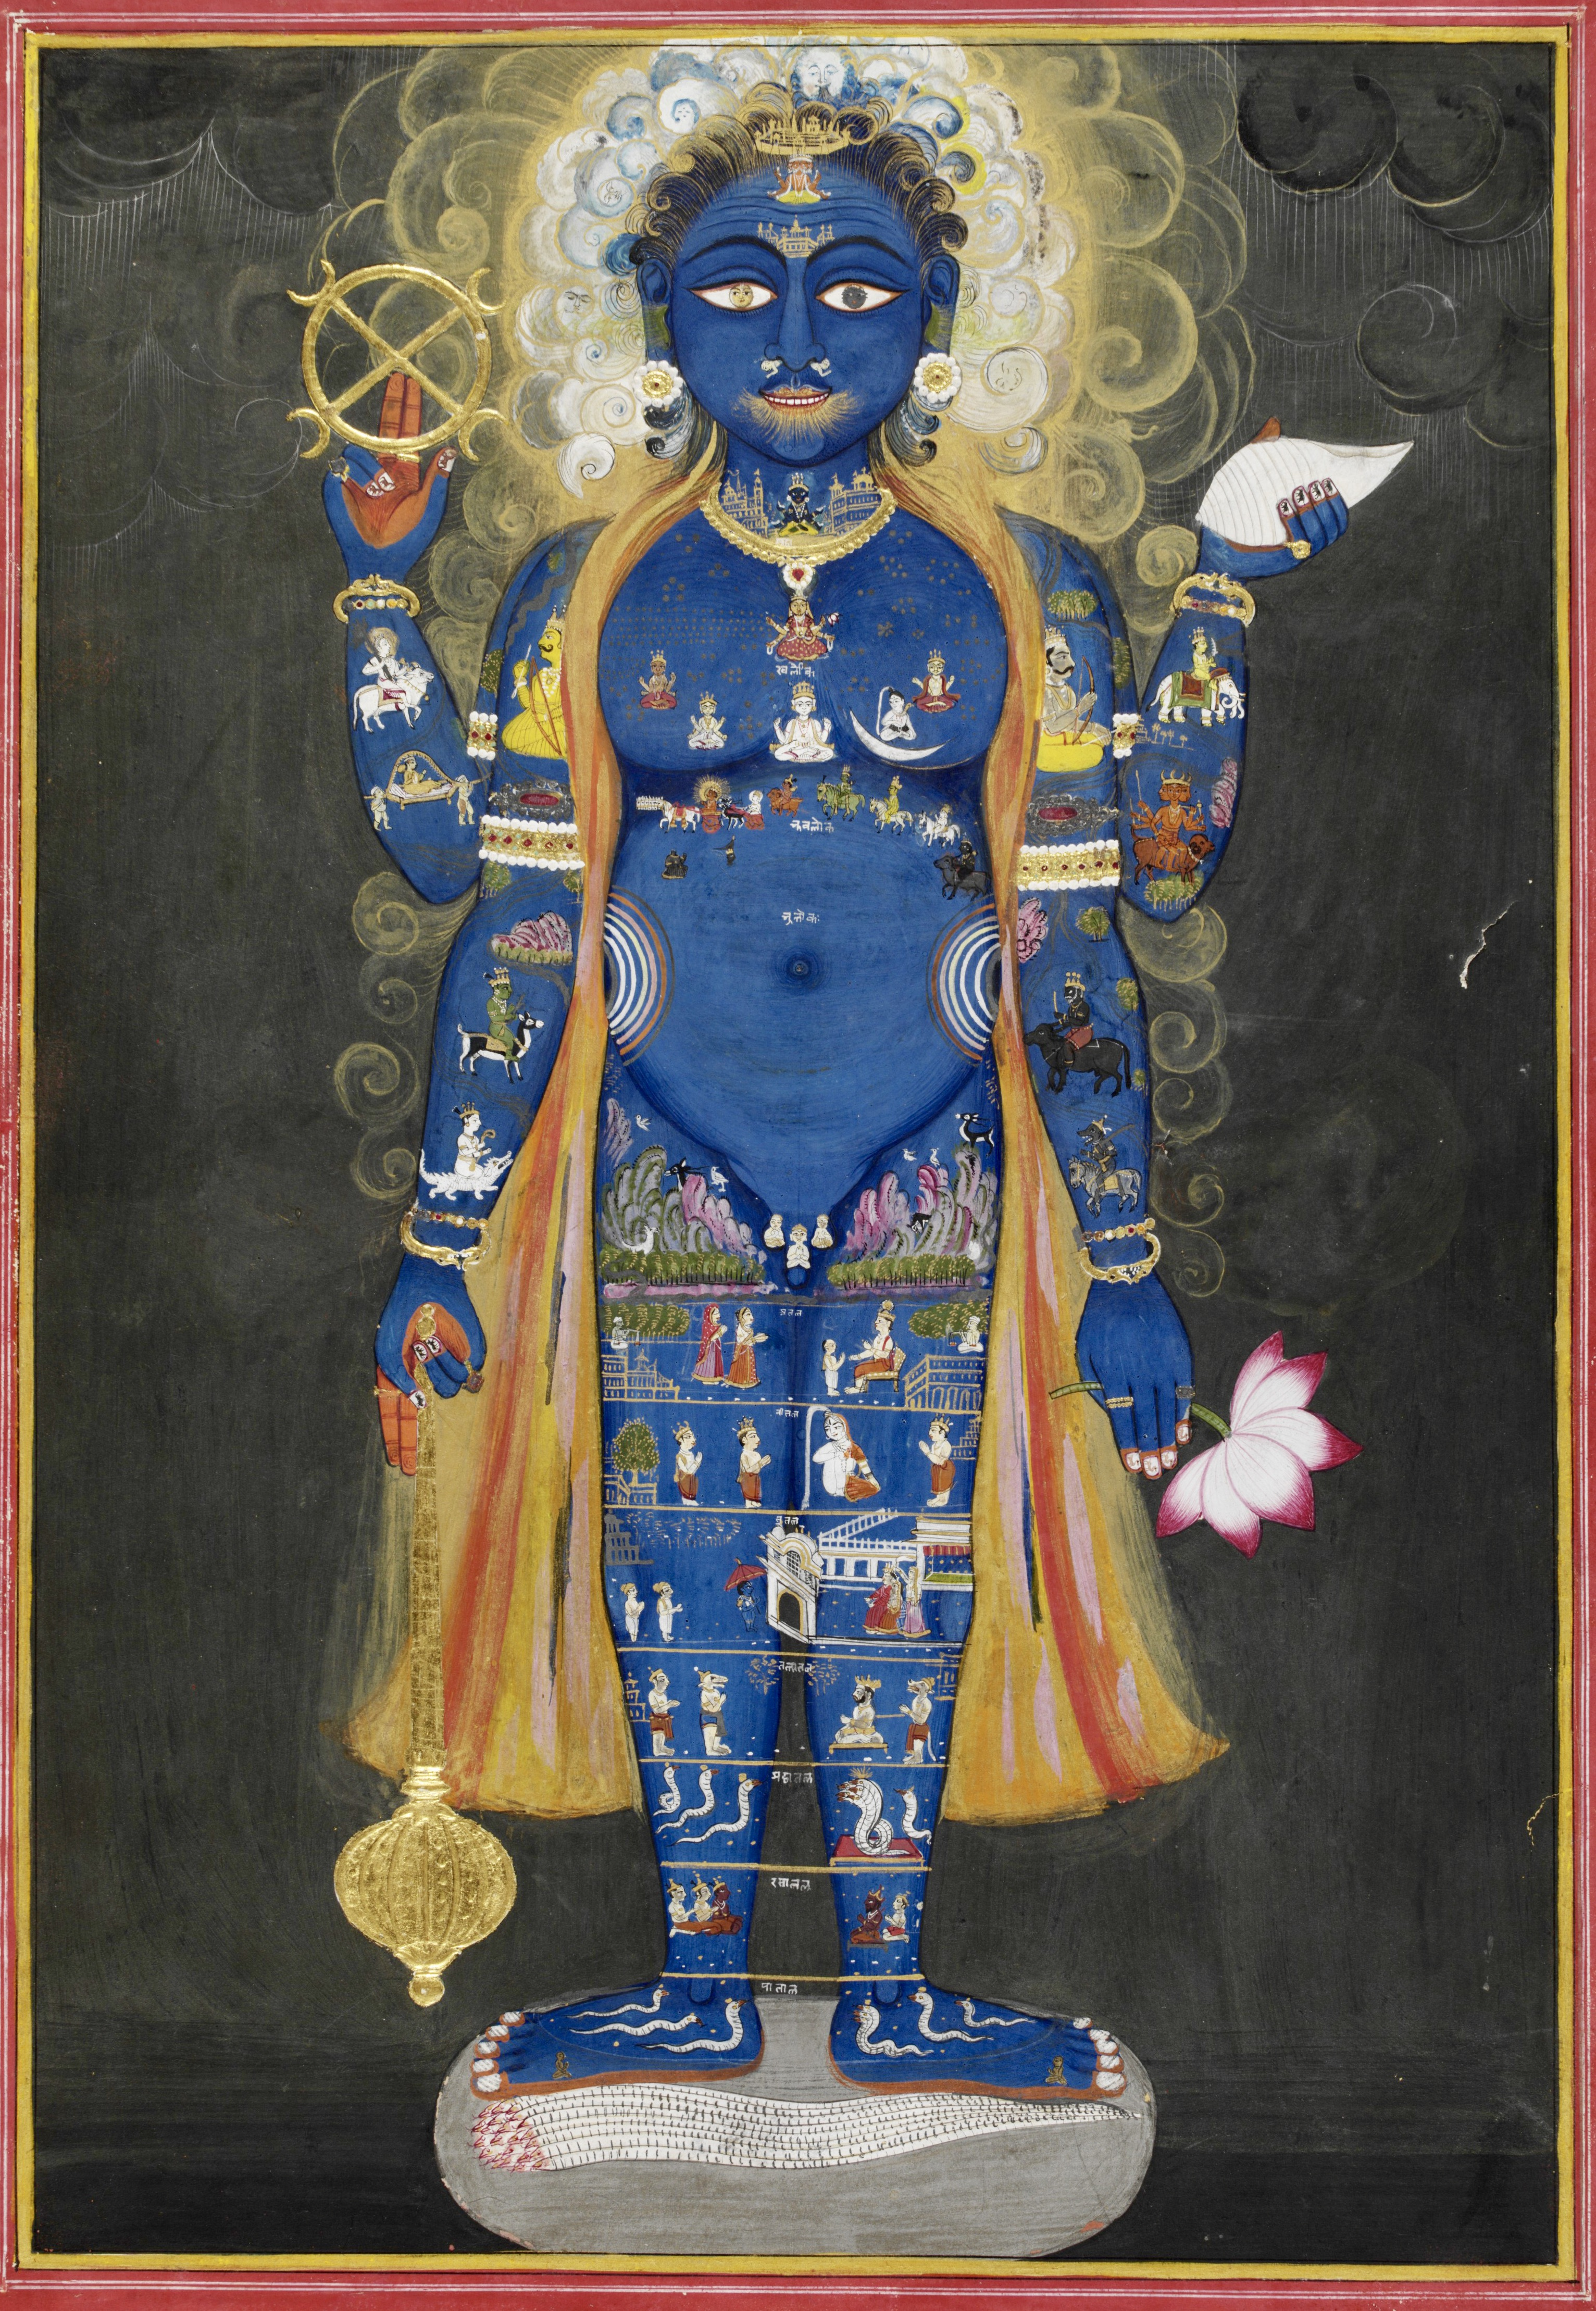
\includegraphics[width=1\textwidth]{pics/Vishnu_Vishvarupa_cropped.jpg}
	\caption{Viṣṇu Viśvarūpa, India, Rajasthan, Jaipur, ca. 1800–1820, Opaque watercolor and gold on paper, 38.5 × 28 cm, Victoria and Albert Museum, London, Given by Mrs. Gerald Clark.}
	\label{fig1}
      \end{figure}
\clearpage
  \begin{figure}[ht]
	\centering
  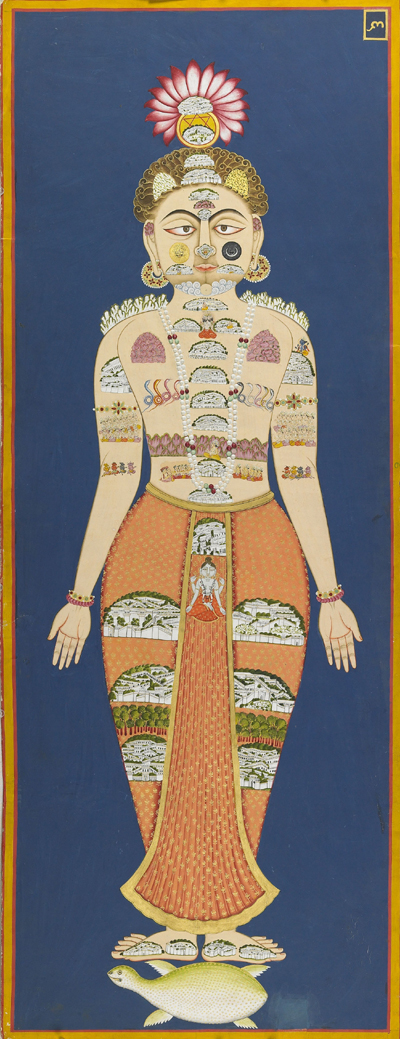
\includegraphics[width=0.5\textwidth]{pics/The_Equivalence_of_Self_and_Universe_(detail),_folio_6_from_the_Siddha_Siddhanta_Paddhati,_(Bulaki),_1824_(Samvat_1881);_122_x_46_cm._Mehrangarh_Museum_Trust..jpg}
	\caption{The Equivalence of Self and Universe (detail), folio 6 from the \textit{Siddhasiddhāntapaddhati} (Bulaki), India, Rajasthan, Jodhpur, 1824 (Samvat 1881), 122 x 46 cm, RJS 2378, Mehragarh Museum Trust.}
	\label{fig2}
      \end{figure}
      % \end{landscape}


\chapter{Bibliography}
 \label{sec:bibli}
   \clearpage
\newpage 
\thispagestyle{empty}
\quad  \addtocounter{page}{-1}

\printbibliography[heading=subbibintoc, title=Consulted Manuscripts, keyword=codex]

\printbibliography[heading=subbibintoc, title=Printed Editions, keyword=printsource]

\printbibliography[heading=subbibintoc, title=Secondary Literature, keyword=seclit]

\printbibliography[heading=subbibintoc, title=Online Sources, keyword=onlinesource]

\end{document}
